% \RequirePackage[ngerman=ngerman-x-latest]{hyphsubst}
% \documentclass[english, BCOR=6mm, twoside=true, open=right, fontsize=12]{tudscrreprt}
\documentclass[english, BCOR=6mm, twoside=true, open=right]{tudscrreprt}
\usepackage[utf8]{inputenc}
\usepackage[english]{babel}
\usepackage{selinput}
\usepackage[T1]{fontenc}
\usepackage{isodate}
\usepackage{graphicx}
\usepackage{pst-all}
\usepackage{mathtools}
\usepackage{latexsym}
\usepackage{amssymb}
\usepackage{threeparttable}
\usepackage{booktabs}
\usepackage{subcaption}
\usepackage{tabularx}
\usepackage{multirow}
\usepackage{glossaries}
\usepackage{pdfpages}
\usepackage{appendix}

% no indent on new paragraph, and set space
\usepackage{parskip}
%change the font
\usepackage[sfdefault,light]{roboto}
%\usepackage[sfdefault]{noto}
\usepackage[T1]{fontenc}
\renewcommand{\baselinestretch}{1.1}

\usepackage{forest}

\definecolor{folderbg}{RGB}{124,166,198}
\definecolor{folderborder}{RGB}{110,144,169}

\def\Size{4pt}
\tikzset{
  folder/.pic={
    \filldraw[draw=folderborder,top color=folderbg!50,bottom color=folderbg]
      (-1.05*\Size,0.2\Size+5pt) rectangle ++(.75*\Size,-0.2\Size-5pt);  
    \filldraw[draw=folderborder,top color=folderbg!50,bottom color=folderbg]
      (-1.15*\Size,-\Size) rectangle (1.15*\Size,\Size);
  }
}



\usepackage{listings}
\usepackage{color}
\definecolor{lightgray}{rgb}{.9,.9,.9}
\definecolor{darkgray}{rgb}{.4,.4,.4}
\definecolor{purple}{rgb}{0.65, 0.12, 0.82}

\lstdefinelanguage{JavaScript}{
  keywords={typeof, new, true, false, catch, function, return, null, catch, switch, var, if, in, while, do, else, case, break},
  keywordstyle=\color{blue}\bfseries,
  ndkeywords={class, export, boolean, throw, implements, import, this},
  ndkeywordstyle=\color{darkgray}\bfseries,
  identifierstyle=\color{black},
  sensitive=false,
  comment=[l]{//},
  morecomment=[s]{/*}{*/},
  commentstyle=\color{purple}\ttfamily,
  stringstyle=\color{red}\ttfamily,
  morestring=[b]',
  morestring=[b]"
}

\lstset{
   language=JavaScript,
   backgroundcolor=\color{lightgray},
   extendedchars=true,
   basicstyle=\footnotesize\ttfamily,
   showstringspaces=false,
   showspaces=false,
   numbers=left,
   numberstyle=\footnotesize,
   numbersep=9pt,
   tabsize=2,
   breaklines=true,
   showtabs=false,
   captionpos=b
}



\usepackage{array}

\newcounter{rowcntr}
\newcolumntype{L}[1]{>{\raggedright\let\newline\\\arraybackslash\hspace{0pt}}p{#1}}
\newcolumntype{C}[1]{>{\centering\let\newline\\\arraybackslash\hspace{0pt}}m{#1}}
\newcolumntype{R}[1]{>{\raggedleft\let\newline\\\arraybackslash\hspace{0pt}}m{#1}}
\newcolumntype{N}[1]{>{\stepcounter{rowcntr}\therowcntr.}R{#1}}

\newcommand{\scaletable}{%
  \begin{tabular}[t]{|*{5}{c|}}%
    \hline
    1 & 2 & 3 & 4 & 5 \tabularnewline
    \hline
  \end{tabular}
}



% pdflatex Glossar.tex
% makeglossaries Glossar
% pdflatex Glossar.tex
\newglossaryentry{Ajax}{
  name=Ajax,
  description={(also AJAX; short for asynchronous JavaScript and XML) is a set of web development techniques using many web technologies on the client-side to create asynchronous Web applications.}
}

\newglossaryentry{SPA}{
  name=SPA,
  description={(Single-page application) is a web application or web site that fits on a single web page with the goal of providing a more fluid user experience similar to a desktop application.}
}

\newglossaryentry{SEO}{
  name=SEO,
  description={(Search engine optimization) is the process of affecting the visibility of a website or a web page in a web search engine's unpaid results.}
}

\newglossaryentry{API}{
  name=API,
  description={(Application programming interface) is a set of routines, protocols, and tools for building software and applications.}
}
\newglossaryentry{CRUD}{
  name={CRUD},
  description={(Create, read, update and delete) are the four basic functions of persistent storage in computer programming. }
}
\newglossaryentry{URI}{
  name={URI},
  description={(Uniform Resource Identifier) is a string of characters used to identify a resource. }
}

\newglossaryentry{ORM}{
  name={ORM},
  description={(Uniform Resource Identifier) is a string of characters used to identify a resource. }
}
\newglossaryentry{MVC}{
  name={MVC},
  description={(Uniform Resource Identifier) is a string of characters used to identify a resource. }
}

\makeglossaries

\begin{document}

\faculty{Department of Computer Science}
% \department{Fachrichtung Strafrecht}
\institute{Institute for Systems Architecture}
\chair{Chair of Computer Networks}
\date{22.07.2016}
\title{Graphical Discussion System}
\subject{master}
\graduation[M.Sc.]{Master of Science}
\author{%
  Kaijun Chen
  \matriculationnumber{3942792}
  \dateofbirth{18.09.1990}
  \placeofbirth{China}
}
\matriculationyear{2013}
\supervisor{Tenshi Hara \and Iris Braun}
\professor{Prof. Dr. rer. nat. habil. Dr. h. c. Alexander Schill}

\maketitle


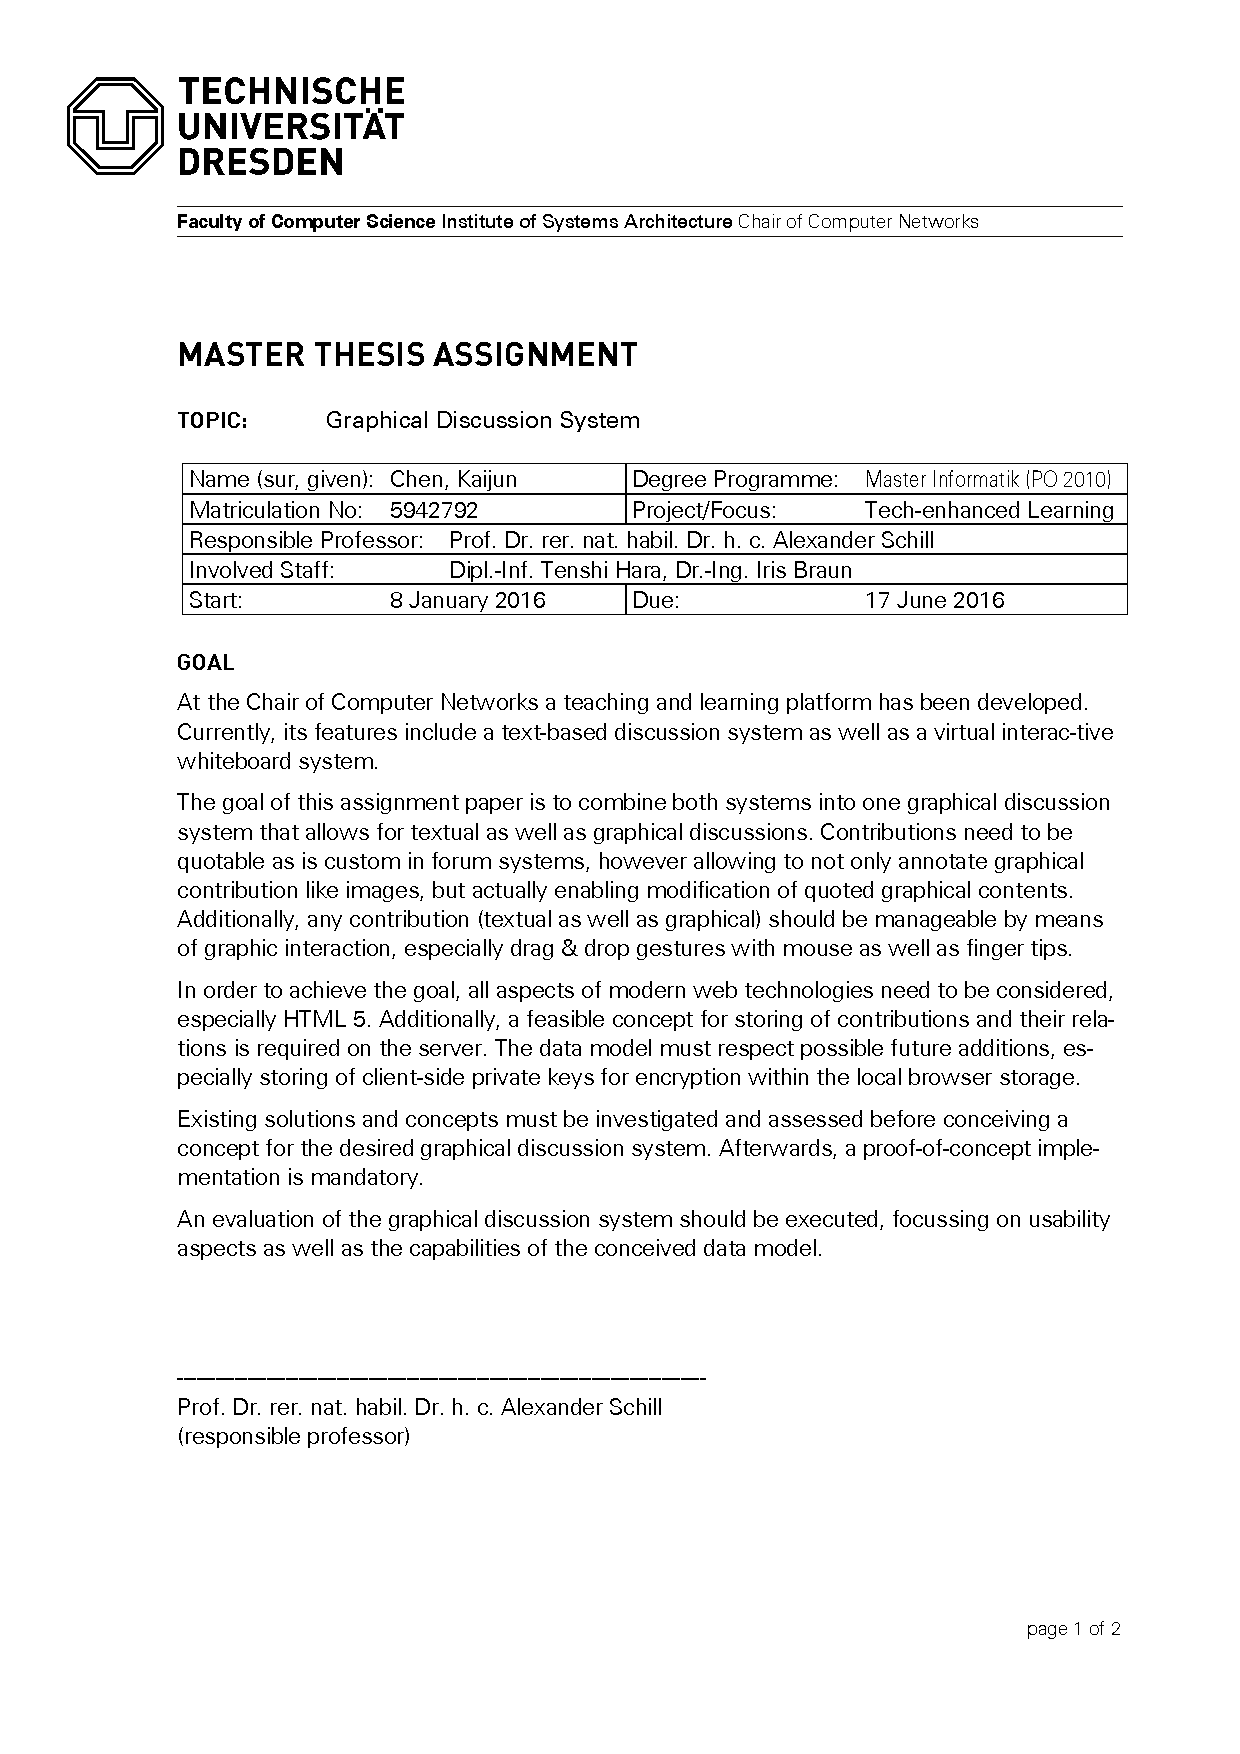
\includepdf[pages={-}]{Documents/KaijunChen-Master-Aufgabenstellung.pdf}

% \confirmation
\confirmation[pagestyle=empty.tudheadings]
\cleardoublepage


% \TUDoption{abstract}{section}
% \begin{abstract}[pagestyle=empty.tudheadings]
% A discussion of the teaching content or the educational material is always essential for both tutors and students in the teaching activities. In traditional way, a discussion can only be performed normally after courses also requires the absence of the students as well as the tutors.

The traditional approach of discussing shows its limitations. Inefficiency in knowledge acquisition: not all the students have the same question and the tutor is able to offer explanation for only one question at same time; time-consumption: ; low interactivity:

Thus, a discuss system with intense interactivity as well as in crowdsourcing way is highly needed. To achieve high interactivity, a discuss system with graphical tool and real-time data communication is proposed. Students are able to contribute their questions and answers to get to the bottom of his deficiencies of teaching content and the educational material. And students who has the same questions can instantly acquire the best solution  which is recommended and approved by the community.

In order to validate and evaluate the concepts of this approach, an implementation of the proposed solution is developed on top of modern web technologies. Moreover, a usability questionnaire survey is proposed and delivered for a quantized evaluation of the client application. The performance of this application is also evaluated at the same time through the created simulation scenarios.

% \end{abstract}

\tableofcontents

% Focus on Discuss System, Graphical, Web-Socket(实时传输)
\chapter{Introduction}
With the rapid development and popularization of internet and technology, the traditional educational activities are moving to the online platforms. MooCs like ..... have taken the responsibilities and ... to .

Tell some histories!

\section{Motivation}
With the rapid development and popularization of the internet and technology, the traditional educational activities are moving to the online platforms.

A discussion of the teaching content or the educational material is always essential for both tutors and students in the teaching activities. However, the traditional approach of discussing shows its limitations. Not all the students have the same question and the tutor is able to offer explanation for only one question at the same time. Moreover, a discussion can only be performed normally after courses also requires the absence of the students as well as the tutor.

Therefore, a discuss system with intense interactivity as well as in crowdsourcing way is highly needed. To achieve high interactivity, a discuss system with graphical tool and real-time data communication is proposed. Students are able to contribute their questions and answers to get to the bottom of his deficiencies of teaching content and the educational material. In addition, students who have the same questions are able to  acquire the best solution instantly which is recommended and approved by the community.

\section{Goals and Research Questions}




This work focuses on the development of a Web-based graphical discussion system, which features storable and quotable graphical discussion contribution. In addition, in order to improve the interactivity of the system which plays a significant role for the educational purpose,real-time communication is also designed. 

Within this thesis the following research questions will be addressed in order to allow the conception, implementation and evaluation of the both client and server sides of graphical discussion system.

\begin{itemize}
  \item How to construct and implement the system with modern Web technologies.
  \item How to design the data model of graphical contribution which is able to be persisted and restored back to sketch board.
  \item How to apply the real-time communication technology to improve the interactivity of the system.
\end{itemize}

\section{Thesis Outline}
This master thesis has the following structure.

\textbf{Chapter 2} gives general introductions of modern Web technologies. The new development process and architecture of Web application are discussed. Afterwards various graphics on the Web are presented and compared. Finally, alternatives of real-time communication technologies are listed.

% \textbf{Chapter 2} shows the latest Android APIs that can be used to access important network parameters. Some research findings about the system information on smartphones are demonstrated and how this information can be accessed. The next section is about some of my own measurements and finally problems occurring during measurements and accuracy of the results are discussed.

\textbf{Chapter 3} considers the general concept of the system. The first section deals with the requirements and mockups with expected functionalities. Thereafter the conception of general architecture is described. In addition, the concept of data model within the system is defined. Finally a feasible concept of serialized graphical data for storing is designed.

\textbf{Chapter 4} covers the implementation of both client and server application of the graphical discuss system. Firstly, general overview about the application structure is given. The storage structure and relation of the data model are shown. At last, the implementation of drawing tool which provides user interfaces for drawing is presented.

\textbf{Chapter 5} obtains the evaluation of system usability and graphical data model. The measurement methodology is introduced and test results are analyzed. 

\textbf{Chapter 6} is the epilogue with a summary of the thesis. The final section discusses future work or researches.


% Focus on Discuss System, Graphical, Web-Socket(实时传输)
% \chapter{Background and Related Works}
% \input{Content/20_RelatedWorks}
% Start With QA system, why nessary -
% \section{Online Q.A. Systems}
% \input{Content/21_QASystems}
% Educational QA System
% \section{MooCs}
% \input{Content/22_MooCs}
% System with Canvas? Socket?


% Focus on Discuss System, Graphical, Web-Socket(实时传输)
\chapter{State of the Art}\label{chapter:state-of-the-art}
The following chapter gives an overview of state of the art. To achieve the high interactivity and responsiveness in the graphical discussion system, a lot of modern web technologies should be applied.

However, there are always plenty of alternatives for each technology which could differ from system to system. So it is important to investigate and analyse the existing solutions and capture an overview about different alternatives of technologies. It's is also vital to understand the benifit and drawback of the technologies used. In addition, a

First of all, the general modern web technology and development workflow will be introduced, which goes through our whole development and has a great impact on the development efficiency. The next part describes the different graphical technologies on web, and which fits our system best. Then an overview of the real time communication technologies is illustrated and evaluated. At last, a collection of modern technologies applied within the backdend server is listed.

\section{Modern Web Development}
% \section{Seperation of Frontend and Backend}


\subsection{Evolution}
With the increasing complexity of a web app and high demand of agile development, people are always thinking about how to improve patterns of the workflow in web development as well as the architecture of a web app. To achieve better scalability, maintainability and ubiquity of a web app, the architecture of an entire web app has been envolving in the past several years .

\subsubsection{Early Age}
At the early age of web development, the backend did all jobs for both client side(browser) and server side, such as rendering, calling system service, composing data, etc. Figure \ref{fig:3.1} shows the overview of web architecture:
\begin{figure}[!htbp]
  \caption{Web architecture in early age}
  \centering
    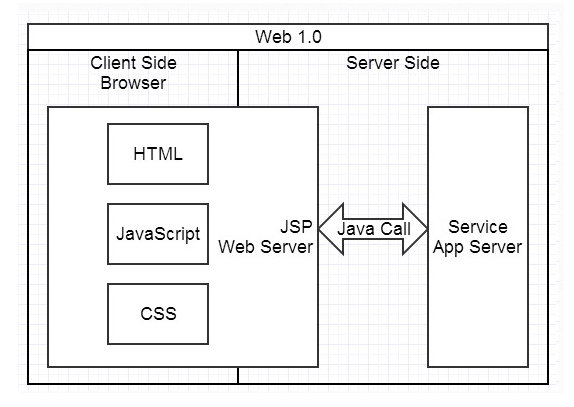
\includegraphics[width=1\textwidth]{Figures/3_1.png}
  \label{fig:3.1}
\end{figure}
The advantage of this pattern is clear: The development and deployment are simple and straightforward, if the bussiness logic doesn't become complexer. But with the increasing complexity of the product, the problems shows up:
\begin{enumerate}
\item
Development of frontend heavily depends on the whore development environment. Developers have to start up all the tools and services for testing and debugging only some small changes on view. In most cases, the frontend developer who isn't familar with the backend needs help while intergrating the new views into the system. Not only the efficiency of development, but also the cost of communication between frontend developer and backend developer are huge problems.
\item
The own responsibility of front-end and back-end mess up, which could be expressed by the commingled codes from different layers, for example there is no clear boundry from data processing tp data representing. The maintainability of the project becomes worse and worse with the increasing complexity.
\end{enumerate}

It's really significant to improve the maintainability of code, as well as the efficiency and resrationality of division of work from both front-end and back-end in the whole web development phase. In the section below, a evolution of the technical architecture will reveal how these problems are solved.

\subsubsection{Web 2.0}
Along with the birth of Gmail\footnote{https://mail.google.com/} in 2004, which is noted for its pioneering use of \gls{Ajax}, the web application started to behave more interactively. Browser began to take over the job of data fetching, processing, rendering, such a sequence of workflow which could only be done by the server side formerly.

The architecture in Web 2.0 generation is presented in figure \ref{fig:3.2}.

\begin{figure}[!htbp]
  \caption{Web 2.0 architecture}
  \centering
    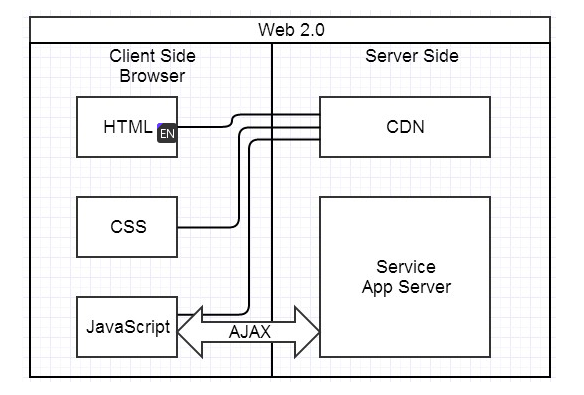
\includegraphics[width=1\textwidth]{Figures/3_2.png}
  \label{fig:3.2}
\end{figure}

By using Ajax, the client has the ability to fetching data stream asynchronously, after which the client will consume the data and render it into the specific section of view. Usability was dramatically improved, because the entired view represented to users will not be refreshed and the front-end is able to process and render data in its own intension, which means more flexible control of the consumption of data.

\subsubsection{Single Page App}

With the evolution of web technologies and promotion of these technologies in modern browswers by brower vendors, a new web development model called \gls{SPA} was proposed and caught the developers' eye. The back-end is no more responsible for rendering and view controling, it only take charge of providing services for the front-end.

\begin{figure}[!htbp]
  \caption{SPA architecture}
  \centering
    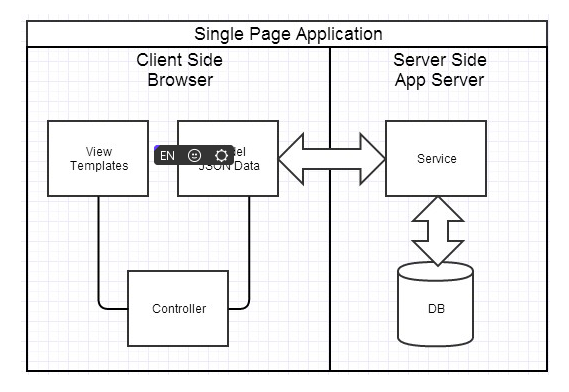
\includegraphics[width=1\textwidth]{Figures/3_3.png}
  \label{fig:3.3}
\end{figure}

The structure in figure \ref{fig:3.3} shows that the client side has the full control of view rendering and data consumption after data acquisition through web services which is released by back-end with promised protocol. All rendering tasks was stripped off from the server side, which means that the server side achieves more efficiency and concentrate more on the core bussiness logics.

But more responsibility in front-end means more complexity. How to reduce the complexity and increace the maintainability of a front-end project becomes a significant problem. Developers come up with an new envolved variant of SPA as demonstrated in figure \ref{fig:3.4}.

\begin{figure}[!htbp]
  \caption{Components in SPA}
  \centering
    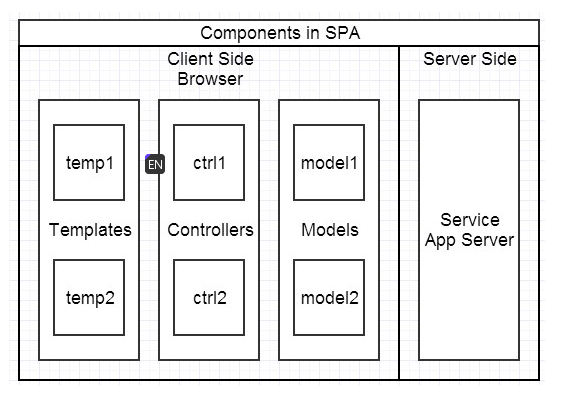
\includegraphics[width=1\textwidth]{Figures/3_4.png}
  \label{fig:3.4}
\end{figure}

In general, the architecture is componentized and layered into template, controller and model. Each component is isolated and has its own view as well as correlated logics. Front-end frameworks like EmberJS, AngularJS, ReactJS are providing such a approach and development pattern for developers to build modern web apps. With this approach, a giant and complex front-end app is broken up into fine grained components, therefore, components are easy to reuse if the components are well abstrated in a proper way. In addition, the maintaince of each component is also effortless.


\subsubsection{Trade-off}
In summarize, a single-page app has a lot of benefits:
\begin{enumerate}
\item
\textbf{Rational seperation of works from front-end and back-end}: client takes charge of view rendering and data representation, as well as slight data processing if needed; the server focus on providing services of the core logics, persistance of data, and also computational tasks.
\item
\textbf{High interactivity and user experience in client side}: asynchronous data fetching and view rendering implies no more need of hard reloading the page which user is viewing and the current states of the page could also be preserved.
\item
\textbf{Efficiency in server side}: rendering tasks are stripped off from server side.
\item
\textbf{Ubiquity}: with the seperation of services provided by server side, not only the web browser but also other clients in other platforms such as Android, iOS apps are able to access and comsume the services.
\end{enumerate}

But SPA also has its deficiencies:

\begin{enumerate}
\item
\textbf{\gls{SEO} unfriendly}: because the page are not directly rendered by server side, and the web crawlers are not able to run JavaScript codes like a browser does, the site could not be crawled properly under normal circumstances. So if SEO results really matter for the app, SPA is obviously not the best choice.
\item
\textbf{Excessive http connections}: all the data is acquired from different services through diversed \gls{API}s, thus multiple HTTP connections are established and performed parallelly, whose initial time of connections for partial data could be much more than a single connection in the traditional way. So it's highly needed to merge the services and find a balance between data model complexity and time consumption.
\end{enumerate}


\subsection{RESTful Interface}

REST is a simple way to organize interactions between independent systems. It's been growing in popularity since 2005, and inspires the design of services, such as the Twitter API. This is due to the fact that REST allows you to interact with minimal overhead with clients as diverse as mobile phones and other websites. In theory, REST is not tied to the web, but it's almost always implemented as such, and was inspired by HTTP. As a result, REST can be used wherever HTTP can.

The alternative is building relatively complex conventions on top of HTTP. Often, this takes the shape of entire new XML-based languages. The most illustrious example is SOAP. You have to learn a completely new set of conventions, but you never use HTTP to its fullest power. Because REST has been inspired by HTTP and plays to its strengths, it is the best way to learn how HTTP works.

\subsubsection{URLs}
URLs are how you identify the things that you want to operate on. We say that each URL identifies a resource. These are exactly the same URLs which are assigned to web pages. In fact, a web page is a type of resource. Let's take a more exotic example, and consider our sample application, which manages the list of a company's clients:

\begin{itemize}
  \item /clients: will identify all clients
  \item /clients/jim: will identify the client, named 'Jim', assuming that he is the only one with that name.
\end{itemize}



In these examples, we do not generally include the hostname in the URL, as it is irrelevant from the standpoint of how the interface is organized. Nevertheless, the hostname is important to ensure that the resource identifier is unique all over the web. We often say you send the request for a resource to a host. 

Finally, URLs should be as precise as needed; everything needed to uniquely identify a resource should be in the URL. You should not need to include data identifying the resource in the request. This way, URLs act as a complete map of all the data your application handles.

\subsubsection{HTTP Verbs}

HTTP verbs tell the server what to do with the data identified by the URL. The request can optionally contain additional information in its body, which might be required to perform the operation - for instance, data you want to store with the resource.

If you've ever created HTML forms, you'll be familiar with two of the most important HTTP verbs: GET and POST. But there are far more HTTP verbs available. The most important ones for building RESTful API are GET, POST, PUT and DELETE. Other methods are available, such as HEAD and OPTIONS, but they are more rare (if you want to know about all other HTTP methods, the official source is IETF).



% \subsection{Continuous Integration}



% \subsection{Operating-system-level virtualization}

% Seperation of Frontend and Backend,
\section{Graphics on the Web}
% Canvas和SVG是HTML5中主要的2D图形技术,前者提供画布标签和绘制API,后者是一整套独立的矢量图形语言,成为W3C标准已经有十多年(2003.1至今),总的来说,Canvas技术较新,从很小众发展到广泛接受,注重栅格图像处理,SVG则历史悠久,很早就成为国际标准,复杂,发展缓慢(Adobe SVG Viewer近十年没有大的更新)

% https://segmentfault.com/a/1190000000490137


% http://stackoverflow.com/questions/5882716/html5-canvas-vs-svg-vs-div


% http://smus.com/canvas-vs-svg-performance/


\subsection{Canvas}

Canvas, which is added in HTML5 as a standard, is an element defined in HTML code with width and height attributes. Graphics can be drawn on Canvas by using HTML5 Canvas APIs via scripting in JavaScript. A full set of drawing functions and helper functions could be used for accessing or rendering pixels on the Canvas area, which also means graphics can be generated dynamically and programmatically. 

Every HTML5 canvas element must have a context. All HTML5 Canvas API to be used are defined within the context. There exits two different types of context in Canvas: 2d context  for drawing 2D graphic and 3d context for 3D graphics. The latter is actually called WebGL and it’s based on OpenGL ES.

The coordinate system of Canvas set the origin offset at the upper-left corner of the canvas, with X coordinates increasing to the right and Y coordinates increasing toward the bottom of the canvas. Which means, the Canvas space doesn’t have points with negative coordinates. 

The significant features of Canvas are listed as follows:

\begin{itemize}
  \item \textbf{Interactivity}: Listeners for keyboard, mouse or touch event are able to be created in the context of Canvas. Users' actions can be captured and response will be made according to the action. 
  \item \textbf{Flexibility}: A variety of shapes like line, rectangle, circle or even text are able to be painted on the Canvas using the native methods. It is also possible to add animations, even video or audio could to the Canvas.
  \item \textbf{Browser/Platform Support}: Unlike Other graphic technology like Flash or Silverlight, which has a very restricted platform support, Canvas is supported by all major browsers which follows the HTML5 standard. In addition, it can be accessed on mobile devices via browser environment.
  \item \textbf{Performance}: Rendering pixels on Canvas is much faster comparing to other graphic technologies on Web\cite{corcoran2011effective}.
\end{itemize}


\subsection{SVG}

SVG is an XML language, similar to XHTML, which can be used to draw graphics, such as the ones shown to the right. It can be used to create an image either by specifying all the lines and shapes necessary, by modifying already existing raster images, or by a combination of both. The image and its components can also be transformed, composited together, or filtered to change their appearance completely\cite{SVGintro}.

Similar with HTML, which provides various elements for defining different styles, SVG provides elements for circles, rectangles, and simple and complex curves. A simple SVG document consists of one \textit{<svg>} element as its root element and several children elements of basic shapes. The composition of elements in SVG builds the graphic. The code listing \ref{list:svg-example-tech} shows a simple example of a SVG element with one rectangle, one circle and a text inside it.

\begin{lstlisting}[language=HTML, caption=Simple Example of SVG elemnt, label={list:svg-example-tech}]
<svg width="300" height="200" >
  <rect width="100%" height="100%" fill="red" />
  <circle cx="150" cy="100" r="80" fill="green" />
  <text x="150" y="125" font-size="60" fill="white">SVG</text>
</svg>
\end{lstlisting}


SVG is natively supported in all modern browsers and also has a good compatibility with old broswers. 

\subsection{Comparision}

\subsubsection{References to already drawn elements}
Since HTML5 Canvas is simply a drawing surface for a bit-map and renders the graphics pixel by pixel, Canvas has no knowledge of the graphics it drew: It doesn’t persist any information of the graphics' properties such as shape, position or size after the graphics were successfully drawn.

On the other hand, SVG maintains references to each object that it renders. Because each SVG element are created and appears in real DOM element on HTML. By default this allows tracking the SVG elements easily and manipulating the every existing element, for example, changing the size of an element or moving the element to another position.

\subsubsection{Rendering Performance}
Those SVG DOM references mean that some of the footwork of dealing with the things you draw is done for you. And SVG is faster when rendering really large objects, but slower when rendering many objects.

A game would probably be faster in Canvas. A huge map program would probably be faster in SVG. If you do want to use Canvas, I have some tutorials on getting movable objects up and running here.

Canvas would be better for faster things and heavy bitmap manipulation (like animation), but will take more code if you want lots of interactivity.

I've run a bunch of numbers on HTML DIV-made drawing versus Canvas-made drawing. I could make a huge post about the benefits of each, but I will give some of the relevant results of my tests to consider for your specific application:

I made Canvas and HTML DIV test pages, both had movable "nodes." Canvas nodes were objects I created and kept track of in Javascript. HTML nodes were movable Divs.

I added 100,000 nodes to each of my two tests. They performed quite differently:

The HTML test tab took forever to load (timed at slightly under 5 minutes, chrome asked to kill the page the first time). Chrome's task manager says that tab is taking up 168MB. It takes up 12-13\% CPU time when I am looking at it, 0% when I am not looking.

The Canvas tab loaded in one second and takes up 30MB. It also takes up 13\% of CPU time all of the time, regardless of whether or not one is looking at it. (2013 edit: They've mostly fixed that)

Dragging on the HTML page is smoother, which is expected by the design, since the current setup is to redraw EVERYTHING every 30 milliseconds in the Canvas test. There are plenty of optimizations to be had for Canvas for this. (canvas invalidation being the easiest, also clipping regions, selective redrawing, etc.. just depends on how much you feel like implementing)

There is no doubt you could get Canvas to be faster at object manipulation as the divs in that simple test, and of course far faster in the load time. Drawing/loading is faster in Canvas and has far more room for optimizations, too (ie, excluding things that are off-screen is very easy).
% Graphics technologies on the web
\section{Real-Time Communication}
% http://stackoverflow.com/questions/10028770/in-what-situations-would-ajax-long-short-polling-be-preferred-over-html5-websock

% HISTORY? BEFORE HTML5

% Short-Polling, Long-Polling
% WebSocket
% WebRTC


\subsection{Long polling}
HTTP Long-polling is a technique used to push updates from server to client. Establishing a connection to server using long polling is like AJAX, but the difference is that the keep-alive connection opens for a certain time period. During the connection persisted, client can retrieve data from the server connected. In case that the connection is closed or timeout unexpectedly, client have to keep requesting periodically in order to reconnect to the Server. On the server side, long polling requests are still treated as HTTP requests same as AJAX. 

Since long polling only uses normal HTTP requests, it is supported in all major browsers.


\subsection{WebSockets}

WebSockets is an advanced technology that provides the possibility to open an interactive communication session between client and server\cite{Websocket}. With the WebSockets API, messages are able to be transmitted to a server and event-driven responses can be returned to client without having to poll the server for a reply.

Starting a WebSockets connection will create TCP connection to server firstly, and keep it as long as needed. The connection can be easily closed by either by server or by client. After the HTTP compatible handshake process has succeeded,  data could be exchanged bi-directionally between server and client. Therefore, WebSockets is suitable for the heavy requirements on frequent data exchange bi-directionally. In addition, message sent through WebSockets is simply encrypted\cite{pimentel2012communicating}.


\subsection{WebRTC}

WebRTC is an industry and standards effort to put real-time capabilities into browser to browser communication and make these capabilities accessible to web developers via standard HTML5 tags and JavaScript APIs\cite{johnston2012webrtc}. 
WebRTC is used to enable the communication between multiple clients. By design, WebRTC allows to transport data in reliable as well as unreliable ways. This is generally used for high volume data transfer such as video/audio streaming where reliability is secondary and few frames or reduction in quality progression can be sacrificed in favour of response time. Both sides (peers) are able to push data to each other independently.

\subsection{Advantages}

The primary advantage of WebSockets is that the connection is not normal HTTP request, but proper message based communication protocol. That allows you to achieve huge performance and architecture advantages. Comparing to long polling, there is no need to start connection mutiple times while using WebSockets. Since the time consumption of establishing a connection is the major part of the total time consumption of a request, reducing the connection numbers will significantly improve the performance and efficiency. 

However, WebRTC is only used for peer to peer connection, but not client to server. Therefore, it is out of the scope of this thesis in general.
% Realtime technologies, comparation of techs
\section{Efficient Client Side}
\subsection{Ember.js}

Ember.js is a popular framework that utilizes a MVC framework composed of views in the form of handlebars templates. In this section, note that there is a bit of work to do in order to facilitate the integration of the templates, models, and controllers. This is not to say that Ember.js is a bad framework, because modification is a byproduct of such a framework.

In Listing 1-1, which is the body of the TodoMVC Ember.js example, you see that the markup consists of two handlebars templates for the to-do list and the to-dos.

Along with these there are three controllers—an app.js entry point, a router,
and a todo input view component. That seems like a lot of files, but in a production environment, that would be minimized. Note the separation of the controllers and views. The views, including the to-do list view shown in Listing 1-2, are quite verbose and make it easy to determine what the code does.


This is a clear example and works as a readable view. There are several properties that are dictated from the controller as you would expect. The controller is named in the router.js file, which also names the view to be used. This controller is shown in the Listing 1-3.

You can see that this TodosListController takes a model of to-dos and adds some properties along with the itemController of 'todo'. This todo controller is actually where most of the JavaScript resides that dictates the actions and conditionals that are visible in the view you saw earlier in this section. As someone who is familiar with Ember. js, this is a well defined and organized example of what Ember.js can do. It is however quite different than React, which you will see soon enough. First, let’s examine a bit of the AngularJS TodoMVC example.

\subsection{AngularJS}

AngularJS is perhaps the world’s most popular MV* framework. It is extremely simple to get started and has the backing of Google along with many developers who have jumped in and created great tutorials, books, and blog posts. It is of course not the same framework as React, which you will soon see. Listing 1-4 shows the AngularJS TodoMVC application.

You can see already that compared to Ember.js, Angular is more declarative in nature in its templating. You can also see that there are concepts like controllers, directives, and services that are tied to this application. The todoCtrl file holds the controller values that power this view. The next example, shown in Listing 1-5, is just a snippet of this file, but you can see how it works.


This example showcases the todoCtrl and shows how it builds a \$scope mechanism that then allows you to attach methods and properties to your AngularJS view. The next section dives into React and explains how it acts on a user interface in a different way than Ember.js and AngularJS do.


\subsection{React}

As you saw in the other examples, there is a basic structure to the TodoMVC applications that makes them an easy choice for demonstrating differences. Ember.js and AngularJS are two popular frameworks that I think help demonstrate that React is not an MV* framework and just a basic JavaScript framework for building user interfaces. This section details the React example and shows you how to structure a React app from the component level, and then works backward to explain how the components are composed. And now, many pages into a book about React, you finally get to see React code in Listing 1-6.

In this example, you see the rendering of the TodoItem component, which is a
subcomponent of the TodoApp. This is simply a component that handles the individual list 14

items that are contained in the TodoApp. This is split off into its own component because
it represents its own set of interactions in the application. It can handle editing as well as marking if the item is completed or not. Since this functionality doesn’t necessarily need to know or interact with the rest of the application, it is built as a standalone component. It may have been just as easy to add to the TodoApp itself initially, but in the world of React, as you will see later, it is often better to make things more modular. This is because in the future the maintenance costs will be recouped by utilizing this logical separation of interactions.
Now you understand at a high level how interactions can often be contained in subcomponents in a React application. The code of the TodoApp render function shows that the TodoItem exists as a subcomponent and shows that the TodoFooter, contained in a JSX by itself, houses its own interactions. The next important concept is to focus on how these subcomponents are reassembled. The TodoItems are added to an unordered list that is contained in a variable called main, which returns the JSX markup for the main section of the TodoApp. Similarly the footer variable contains the TodoFooter component. These two variables, footer and main, are added to the return value of the TodoApp, which you see at the end of the example. These variables are accessed in JSX by using curly braces so you see them as follows:


\subsection{Why React.js}

In many cases when you learn something, you first need to realize what the thing is that you are learning. In the case of React, it can be helpful to learn which concepts are not parts of the React framework. This will help you understand which standard practices you have learned need to be unlearned, or at least need to be set aside, in order to fully understand the concepts of a new framework such as React. So what is it that makes React different and why is it important?

Many argue that React is a full-scale JavaScript framework on a level that compares to other frameworks such as Backbone, Knockout.js, AngularJS, Ember, CanJS, Dojo, or any of the numerous MVC frameworks that exist. Figure 1-1 shows an example of a typical MVC framework.

Figure 1-1 shows the basics of each of the components in a Model-View-Controller architecture. The model handles the state of the application and sends state-changing events to the view. The view is the user-facing look and interaction interface to the end user. The view can send events to the controller, and in some cases to the model. The controller is the main dispatcher of events, which can be sent to the model, to update state, and the view to update the presentation. You may note that this is a generic representation of what an MVC architecture is, and in reality there are so many variants and customized implementations that there is no single MVC architecture. The point isn’t to state what an MVC structure looks like, but to point out what React is not.

This MVC structure is actually not a fair assessment of what React is or intends to be. That is because React is one particular piece of what these frameworks present. React is in its simplest form, just the view of these MVC, MVVM, or MV* frameworks. As you saw in the previous section, React is a way to describe the user interface of an application and a mechanism to change that over time as data changes. React is made with declarative components that describe an interface. React uses no observable data binding when building an application. React is also easy to manipulate, because you can take the components you create and combine them to make custom components that work as you expect every time because it can scale. React can scale better than other frameworks because of the principles that drove it from its creation. When creating React interfaces, you structure them in such as way that they are built out of multiple components.

Let’s pause for a minute and examine the most basic structure of several frameworks and then compare them to React in order to highlight the differences. For each of the frameworks, you will examine the most basic to-do list applications as they are created for the http://todomvc.com web site. I am not going to deride other frameworks because they all serve a purpose. Instead I attempt to demonstrate how React is structured compared to the others. I showcase just the important parts to highlight and limit a complete recreation of the application here. If you want to see the full examples, the links to the source are included. Try not to become too focused on the implementation details of any of these examples, including the React example, because as you progress through this book the concepts will be covered thoroughly and will help you understand what is going on completely.
% Tech stack: React, Babel, ES6, ...
\section{Efficient Server Side}
This section gives the explanation of architectural pattern and more detailed implementation of the server side. 

% Architecture MV, , JWT for Auth, Websocket Dispatcher, Resource Listening?

\subsection{Architecture}

\subsubsection{MVC Pattern and Project Structure}
To separate the different layers of model, view and controller, \gls{MVC} pattern is used as the basic pattern of the architecture. In the model layer, all data model related concerns such as data shema definitions, data model validation as well as database operations are defined. And Controllers contain the core domain logics, process the data from model layer, and pass the result to view layer.

Since the templates are rendered on the client side, the view layer is just simply stripped. Therefore, basically the controllers response processed data to client side directly without rendering it to views. Figure \ref{fig:server-file-structure-imp} shows the overview of the server's  file structure which is featured with MVC pattern.

\begin{figure}[!htbp]
\centering
\begin{forest}
  for tree={
    font=\ttfamily,
    grow'=0,
    child anchor=west,
    parent anchor=south,
    anchor=west,
    calign=first,
    edge path={
      \noexpand\path [draw, \forestoption{edge}]
      (!u.south west) +(7.5pt,0) |- node[fill,inner sep=1.25pt] {} (.child anchor)\forestoption{edge label};
    },
    before typesetting nodes={
      if n=1
        {insert before={[,phantom]}}
        {}
    },
    fit=band,
    before computing xy={l=15pt},
  }
[server
  [config/
    [index.js]
    [routes.js]
  ]
  [models/]
  [controllers/]
  [index.js]
  [...]
]
\end{forest}
\caption{Overview of server app's file structure}
\label{fig:server-file-structure-imp}
\end{figure}


\begin{enumerate}
\item 
  \textbf{index.js}: the entry point of the whole server app. It will create a server instance and set up configurations for the server. In addition, a connection from server instance to database will be established. After all configurations are done, the server instance will start listening port and waiting for the requests from client.
\item
  \textbf{config/index.js}: config as well as constants for the server. It persists \textit{apiConfig} for example the common prefix of API URL and version of the API. And config for database including the database URL will be defined here as well. In addition, keys for encryption are also stored in the config file.
\item
  \textbf{config/routes.js}: rules for URL matching. All URL matching rules are defined in this file. Controllers are referenced here and a dispatcher for router will be instantiated. If any request meets the defined rule, the request will be forward to a correlative controller. 
\item
  \textbf{controllers/*}: controllers for processing specific requests.
\item 
  \textbf{models/*}: data model definitions. Files under this directory are organized by different data domain.
\end{enumerate}


\subsubsection{Achitecture of Server}

The figure \ref{fig:server-arch-imp} illustrates an overview of the server's architecture. 

\begin{figure}[!htbp]
  \centering
    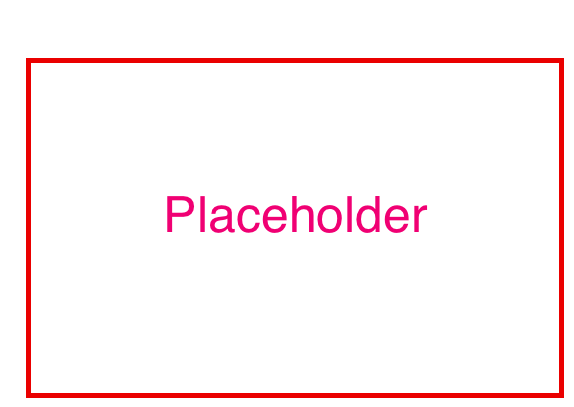
\includegraphics[width=0.6\textwidth]{Figures/placeholder.png}
  \caption{placeholder}
  \label{fig:server-arch-imp}
\end{figure}
% process of request to be handeled. index.js -> create server isntance -> connect to database. routes -> different controllers -> different models

\subsection{Data Schema Definition}
% Tech stack: Nodejs (Why Node, comparation), MongoDB(Why, comparaion), Express?


\section{Conclusion}

TBD

% At least to 32-35

% \chapter{Requirements}\label{sec:aims}
% Before starting to concept the graphical discuss system, it's necessary to analyse requirements and objectives behind the origin motivation in the first place. It should be defined at first, what kind of functionalities should be achieved and how the system behaves.

\section{Basic Functionalities}

As a graphical discuss system for the educational purpose, the system should contain basic functionalities on the prototype  of a forum which could be organized by classes. So class management, question management and answer management are the three essential parameters to be designed at the start.

\subsection{Course Management}

Each question should have a certain domain of its content, so the questions are organized by classes initially. The features of course management should be:

\begin{enumerate}
\item
\textbf{Create Course}: The user who is identified as a tutor is able to create course and maintain the course he created. While creating the course, the tutor can define the name of the course and upload an image as a background of the course for better recognization. In addition, concret description of the course could also be added to the description area.

\begin{figure}[!htbp]
  \centering
    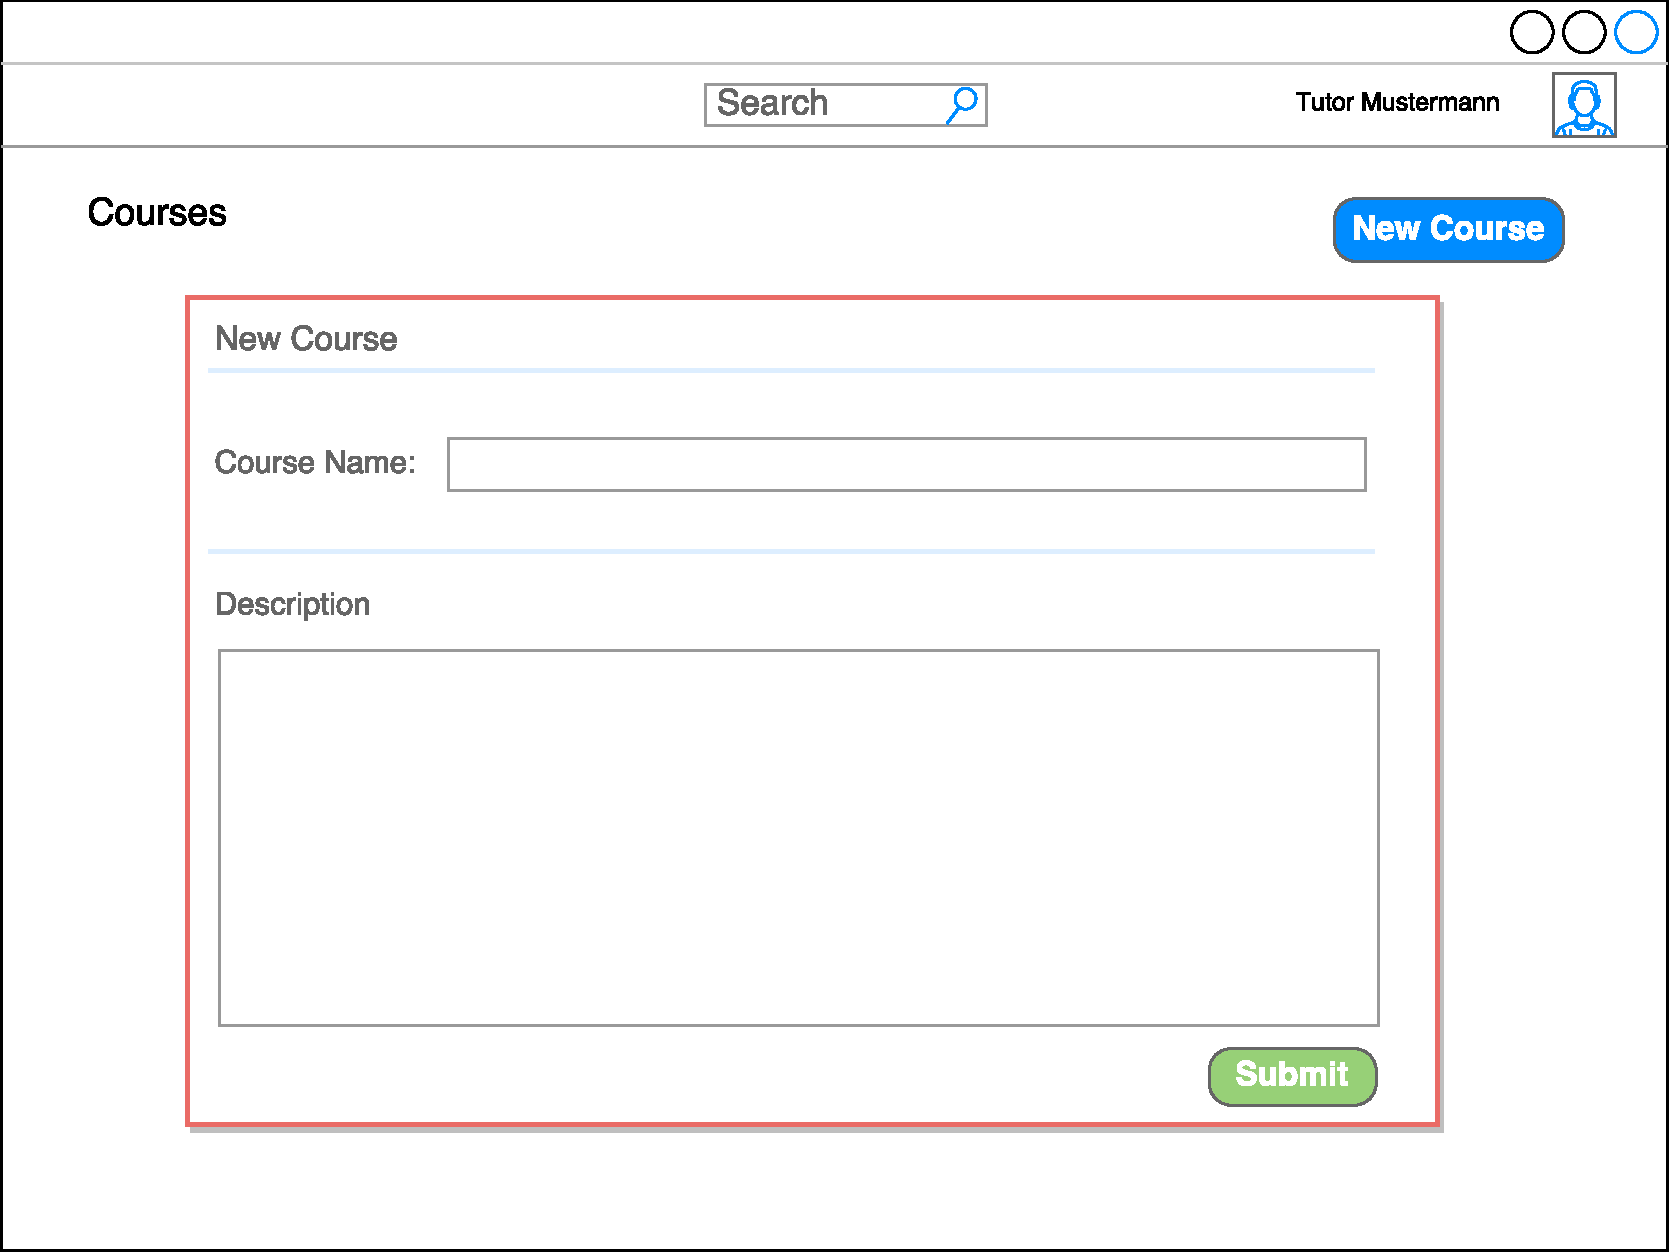
\includegraphics[width=0.8\textwidth]{Figures/mockup/add-new-course.pdf}
  \caption{Submit a new course}
\end{figure}

% Mockups create, upload, description

\item
\textbf{Search Course}: After a course is created, a corresponding unique identifier code for the course will be generated at the same time. The students are able to find the course through the identifier code.

\begin{figure}[!htbp]
  \centering
    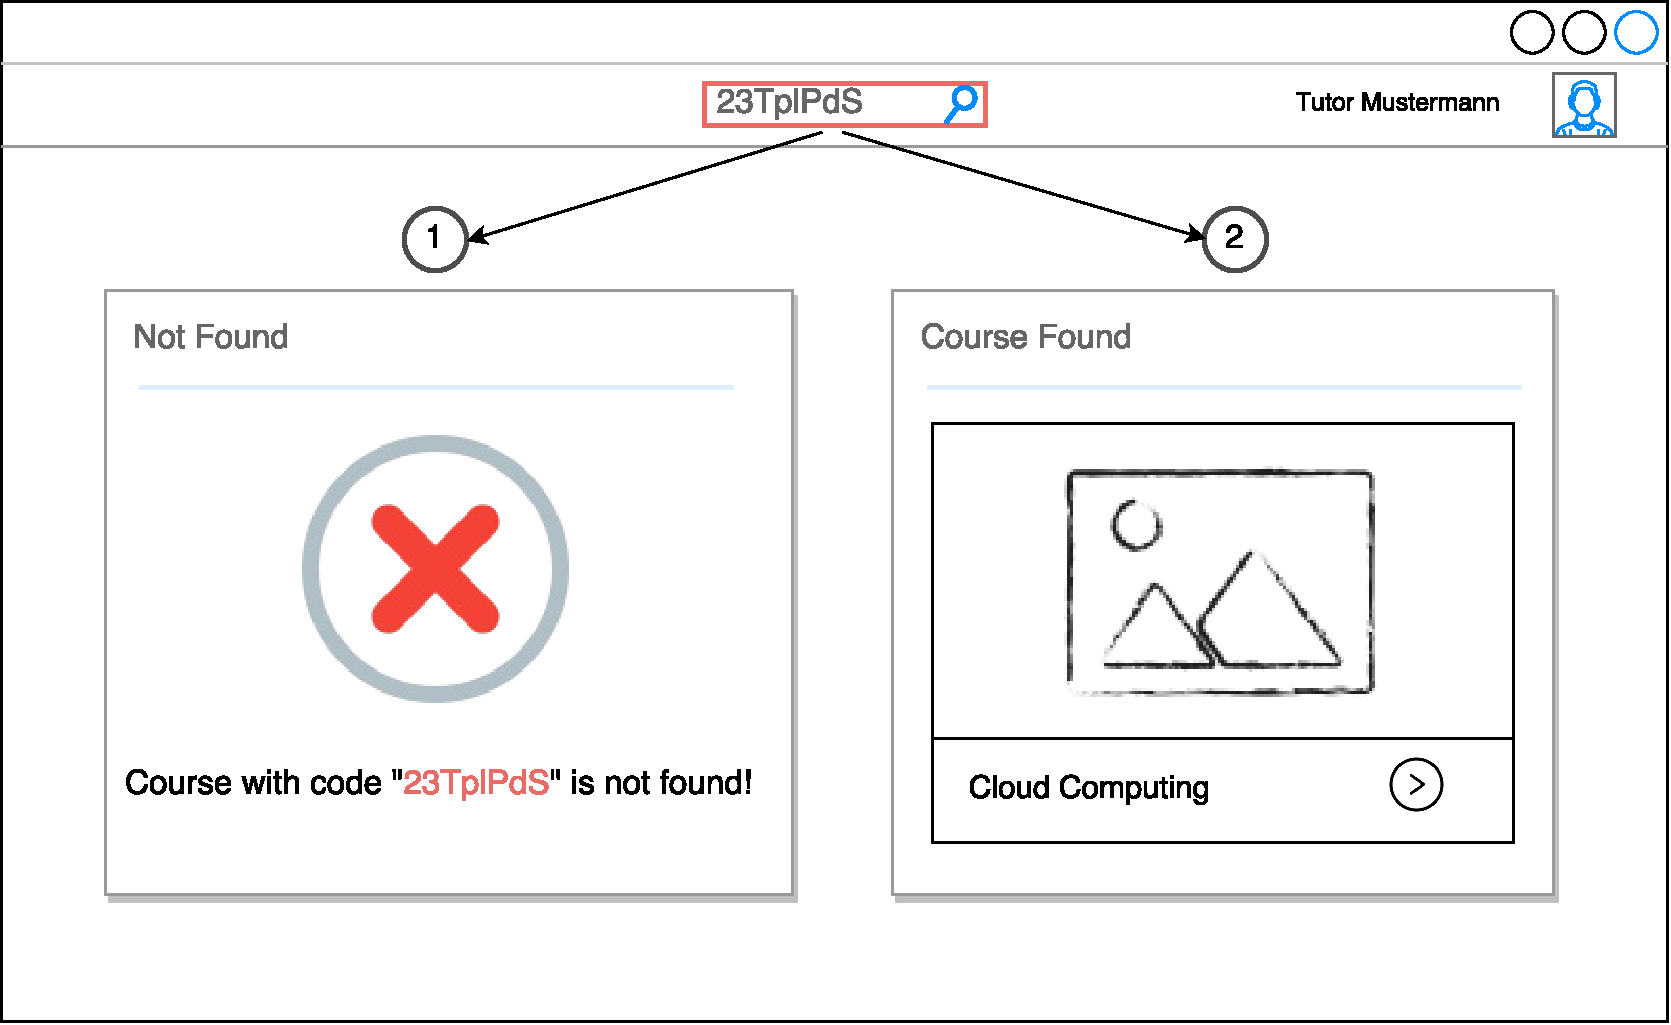
\includegraphics[width=0.8\textwidth]{Figures/mockup/Search-Course.pdf}
  \caption{Search course with code}
\end{figure}
% Mockups code, search

\item
\textbf{Favor Course}: If a student is interest to a certain course, he is capable to add the course to his favor list so that it's easy to find and access the course he liked later.

\begin{figure}[!htbp]
  \centering
    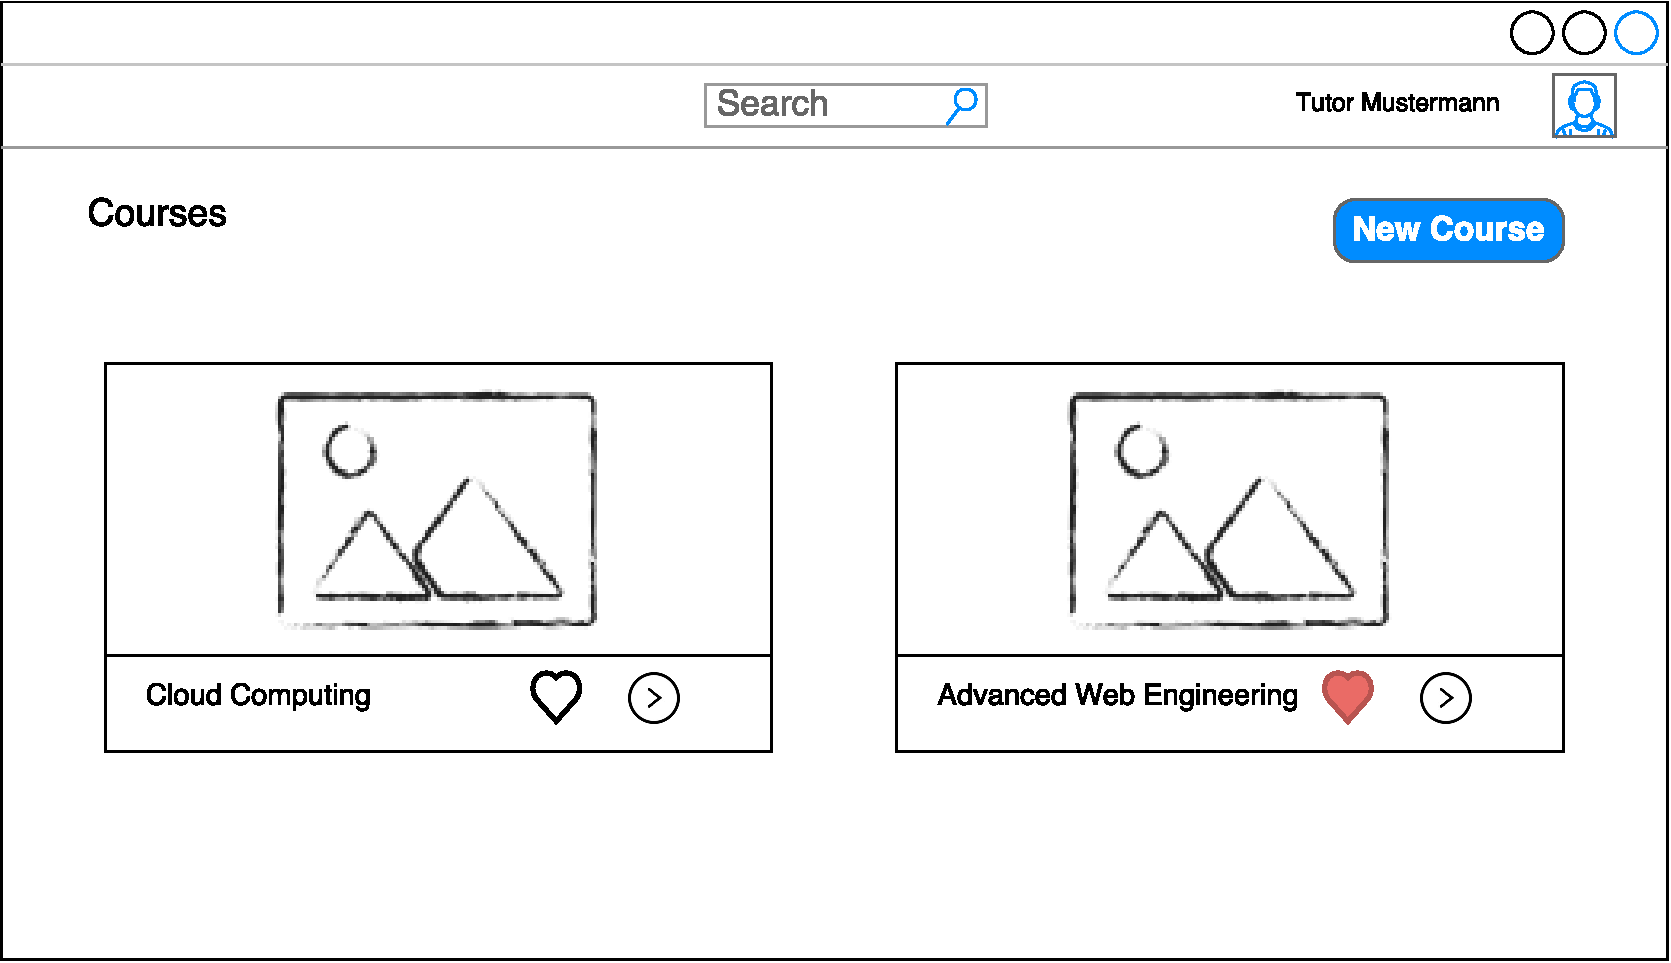
\includegraphics[width=0.8\textwidth]{Figures/mockup/Favour-Course.pdf}
  \caption{Favor course}
\end{figure}
% Mockups fav button, fav list.

\end{enumerate}

\subsection{Question Management}

\begin{enumerate}
\item
\textbf{Submit/Edit/Withdraw Question}: The student who has confusion with the teaching content can submit his own question with detailed description in a certain course. The user is also permitted to edit the question if he want to add more precise informations or modify the unclarity he made to the question. Withdrawing of his own question is also possible, but only when there're no contributes made to the question.

\begin{figure}[!htbp]
  \centering
    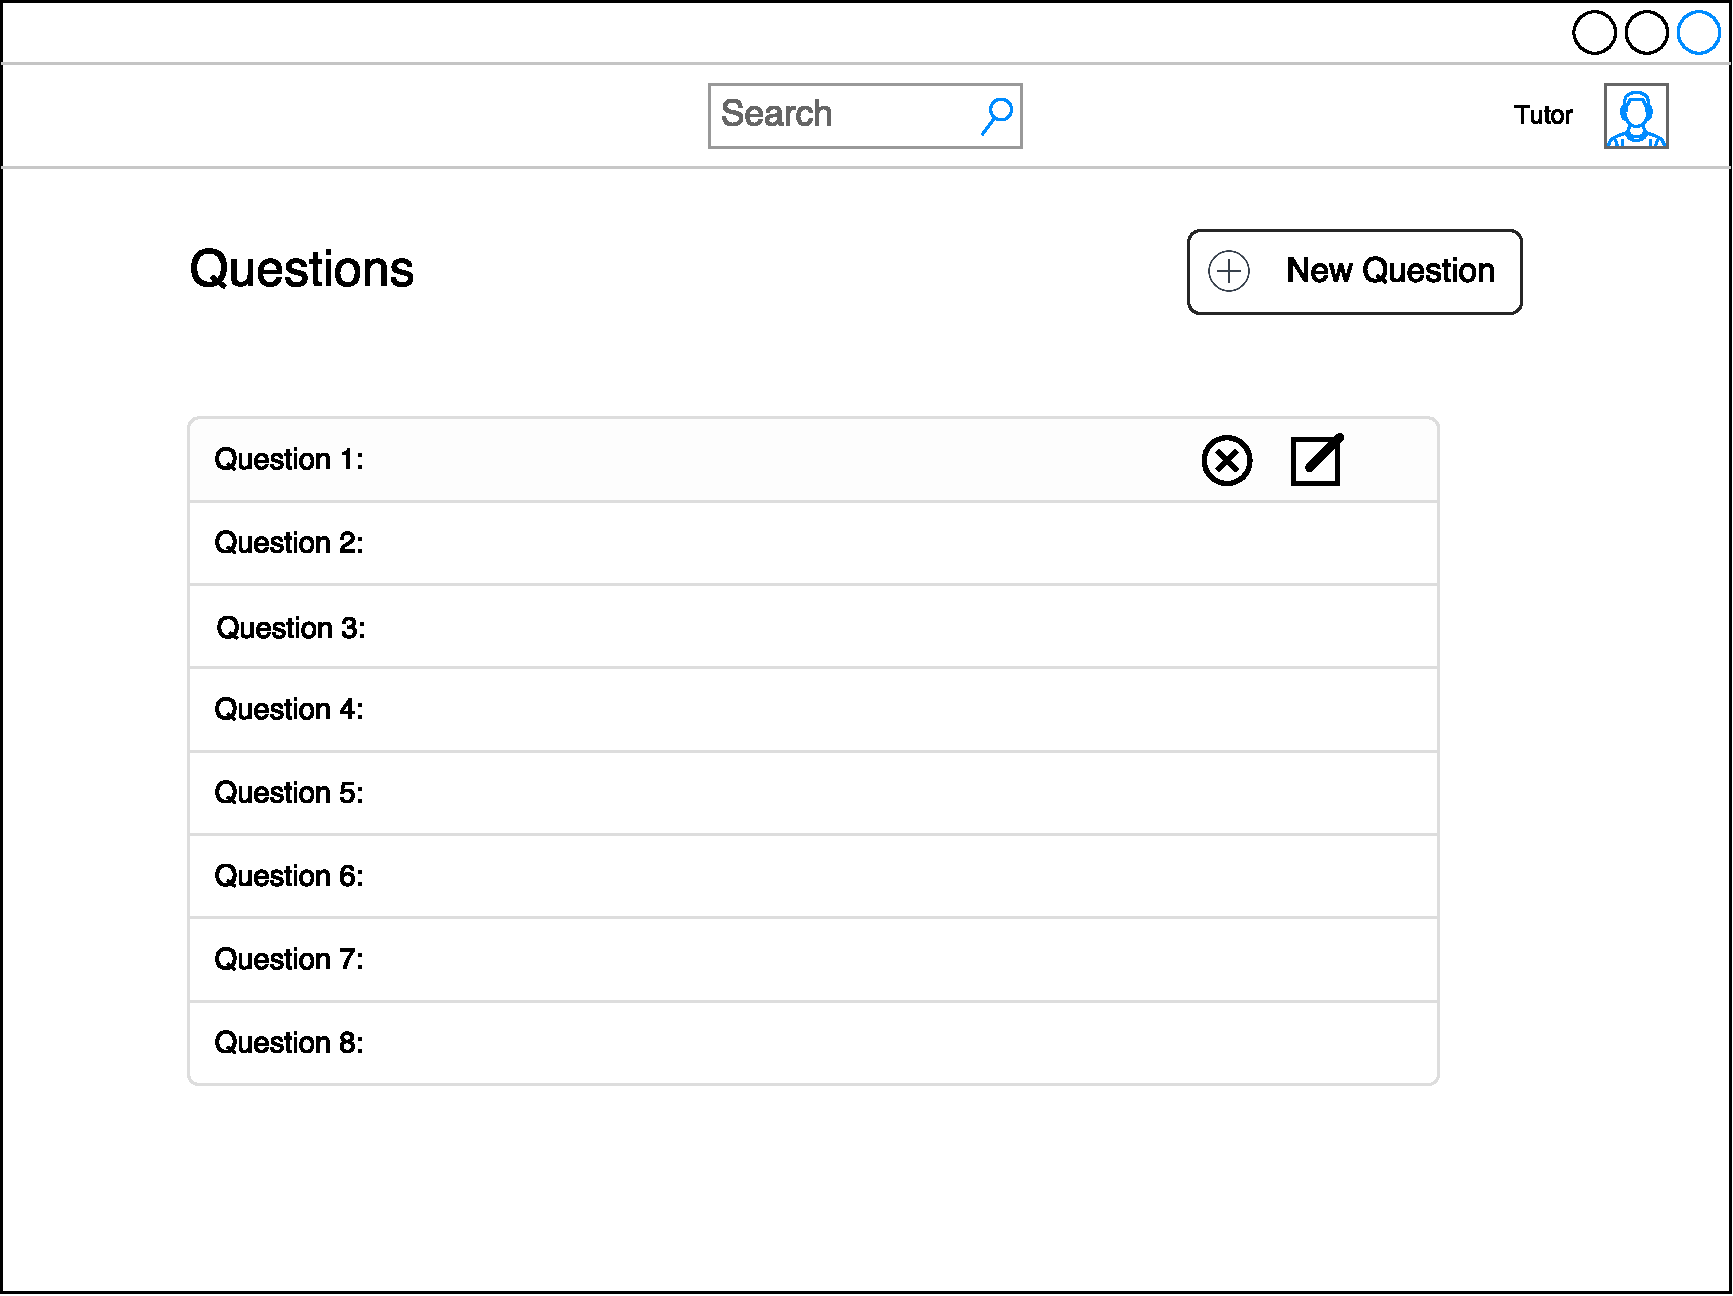
\includegraphics[width=0.8\textwidth]{Figures/mockup/New-question.pdf}
  \caption{Submit a new question; withdraw or modify own question}
\end{figure}
% Mockups submit/Edit, withdraw

\item
\textbf{Upvote/Downvote Question}: An assessment of a question is decisive for building a better community with high-quality contents. So the user is able to upvote or downvote of a question and determine if the question is helpful for other members in the community or not.

\begin{figure}[!htbp]
  \centering
    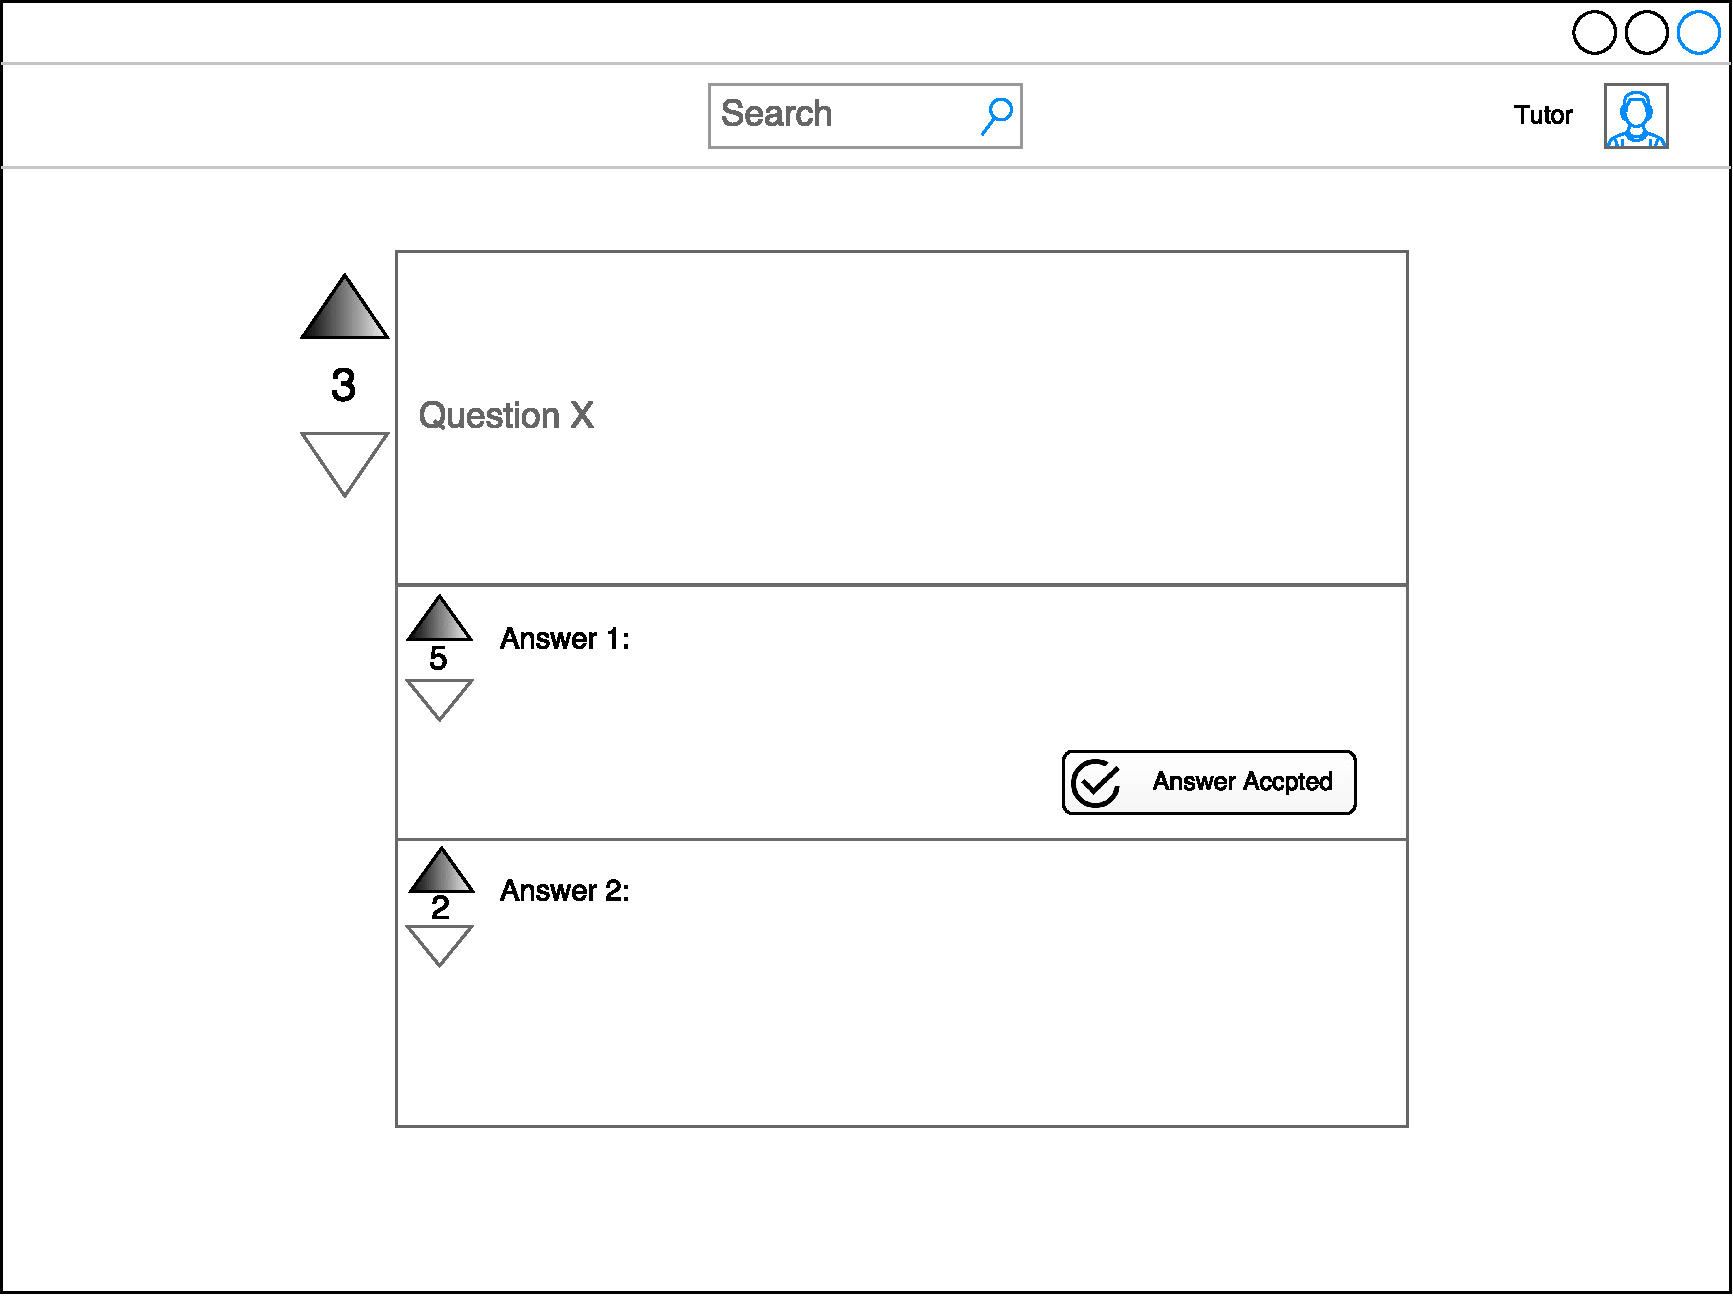
\includegraphics[width=0.8\textwidth]{Figures/mockup/question-vote.pdf}
  \caption{Upvote/Downvote a question or answer}
\end{figure}
% Mockups Upvote/downvote.

\item
\textbf{Favor Question}: If the student consider the question as a helpful and useful content and want to review this question in the future, he can favor the question and locate it in a certain list.

% \begin{figure}[!htbp]
%   \caption{placeholder}
%   \centering
%     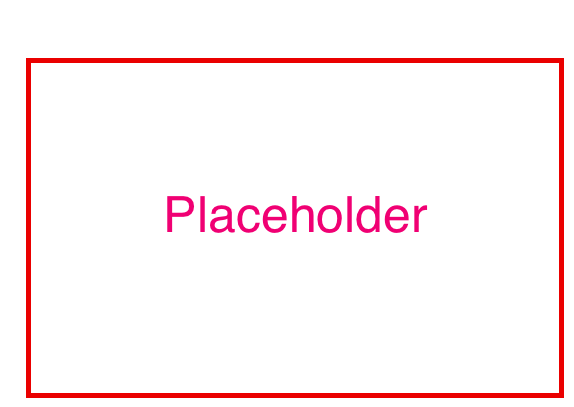
\includegraphics[width=0.8\textwidth]{Figures/placeholder.png}
%   \label{fig:placeholder}
% \end{figure}
% Mockups Fav, fav list

\item
\textbf{Accept Answer}: The owner of the question has the right to accept the most useful answer in his opion which will be shown up at the top of the answer list.

% \begin{figure}[!htbp]
%   \caption{placeholder}
%   \centering
%     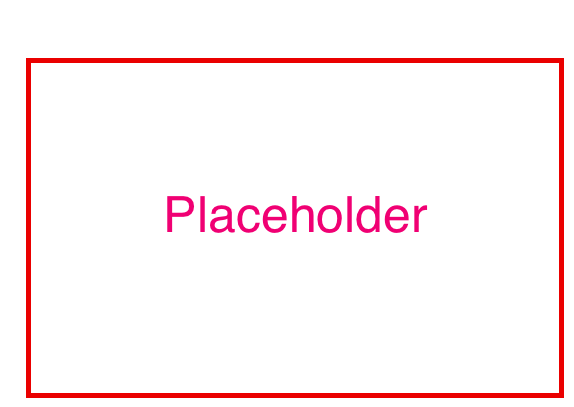
\includegraphics[width=0.8\textwidth]{Figures/placeholder.png}
%   \label{fig:placeholder}
% \end{figure}
% Mockups Accept, Top.

\end{enumerate}

\subsection{Answer Management}

\begin{enumerate}
\item
\textbf{Submit/Modify/Remove Answer}: User who has experence with the question can submit his answer to the question. After the submission, the modification or removal of the user's own question is possible.

\begin{figure}[!htbp]
  \centering
    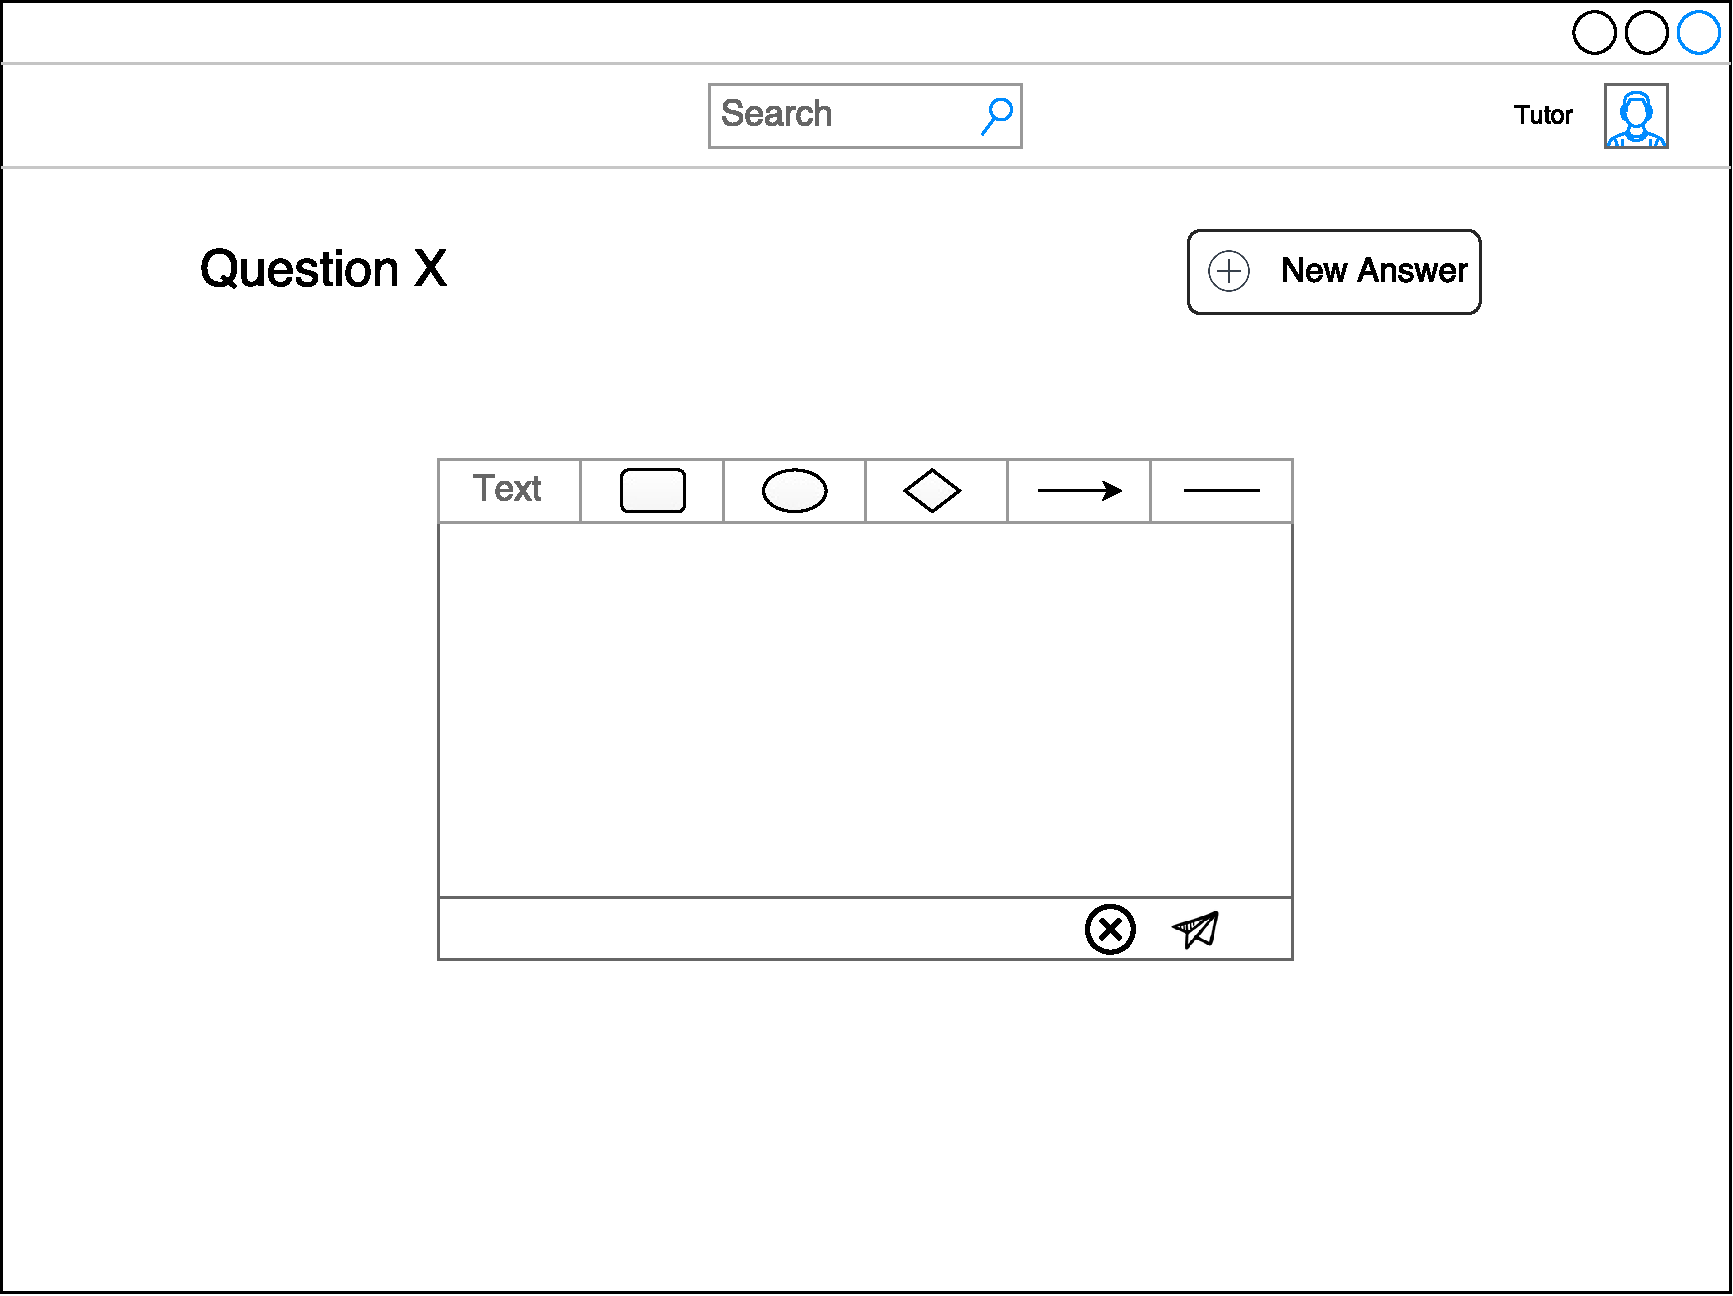
\includegraphics[width=0.8\textwidth]{Figures/mockup/New-Answer-modify.pdf}
  \caption{Submit a new answer}
\end{figure}
% Mockups submit, withdraw

\item
\textbf{Upvote/Downvote Answer}: As mentioned above in section of question functionality, a similar idea of assessment should also be applied to answers. Answer with higher vote will be listed at first.

% \begin{figure}[!htbp]
%   \caption{placeholder}
%   \centering
%     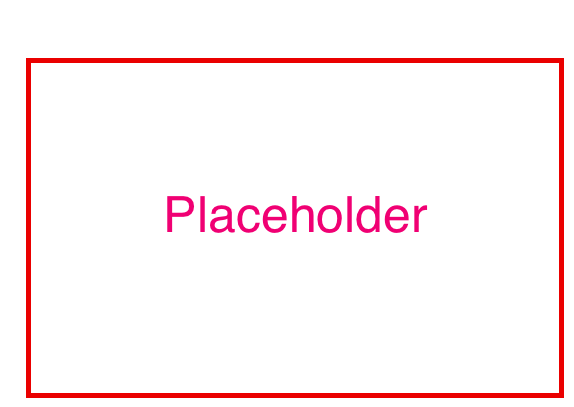
\includegraphics[width=0.8\textwidth]{Figures/placeholder.png}
%   \label{fig:placeholder}
% \end{figure}
% Mockups Upvote/downvote, arrange of answer.

\item
\textbf{Quote Answer}: Answers are able to be quoted so that the user can supplement informations on the top of original post or point out the deficiency of the contribute.

\begin{figure}[!htbp]
  \centering
    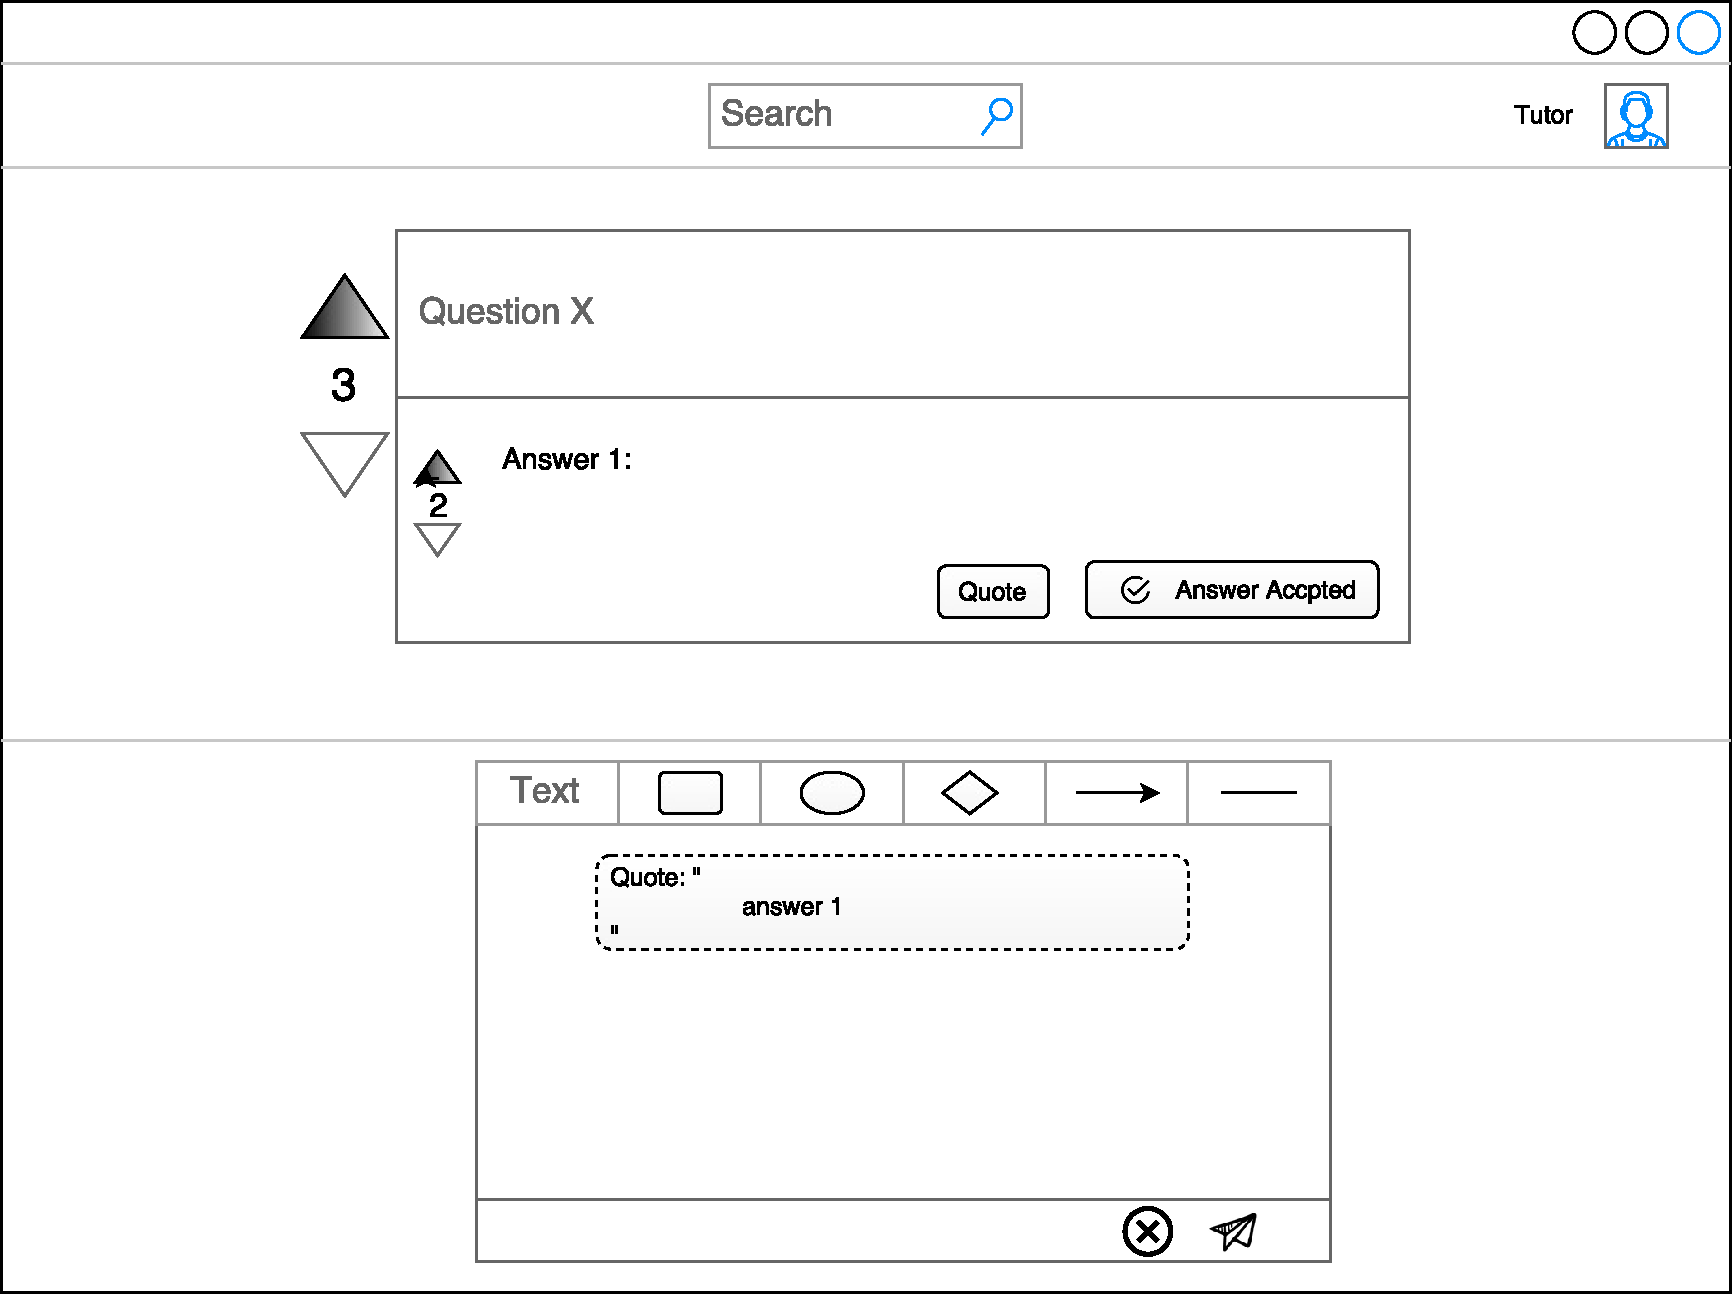
\includegraphics[width=0.8\textwidth]{Figures/mockup/quote.pdf}
  \caption{Quote an answer}
\end{figure}
% Mockups Fav, fav list

\end{enumerate}


\section{High Interativity}
Building with the basic functionalities is far not enough. To fit the system for educational purpose and improve the interactivity for arousing enthusiasm of students, a drawing tool and realtime functionality should be intergrated into the system.

\subsection{Drawing Tool}
Normally, some of the thoughts can't be simply expressed by textual description, so a drawing tool should be designed to enables the user to compose not only text but also different components such like rectangle, circle, line and so on, which helps the user to express his question more precisely.
The ideal drawing tool should have following features:

\begin{enumerate}
\item
\textbf{Drawing Diverse Components}: Not only text but also diverse components could be drawn while posting a contribution. Styling of a component such as size tuning, color changing is also the essential, which will helps emphasize the important part the user expressing.

\item
\textbf{Drawing History}: During drawing, the user might make mistakes or change mind after placing a component or text. So a history list of drawing actions bundled with undo and redo functionalities will dramatically improve the usability of drawing process.

\begin{figure}[!htbp]
  \centering
    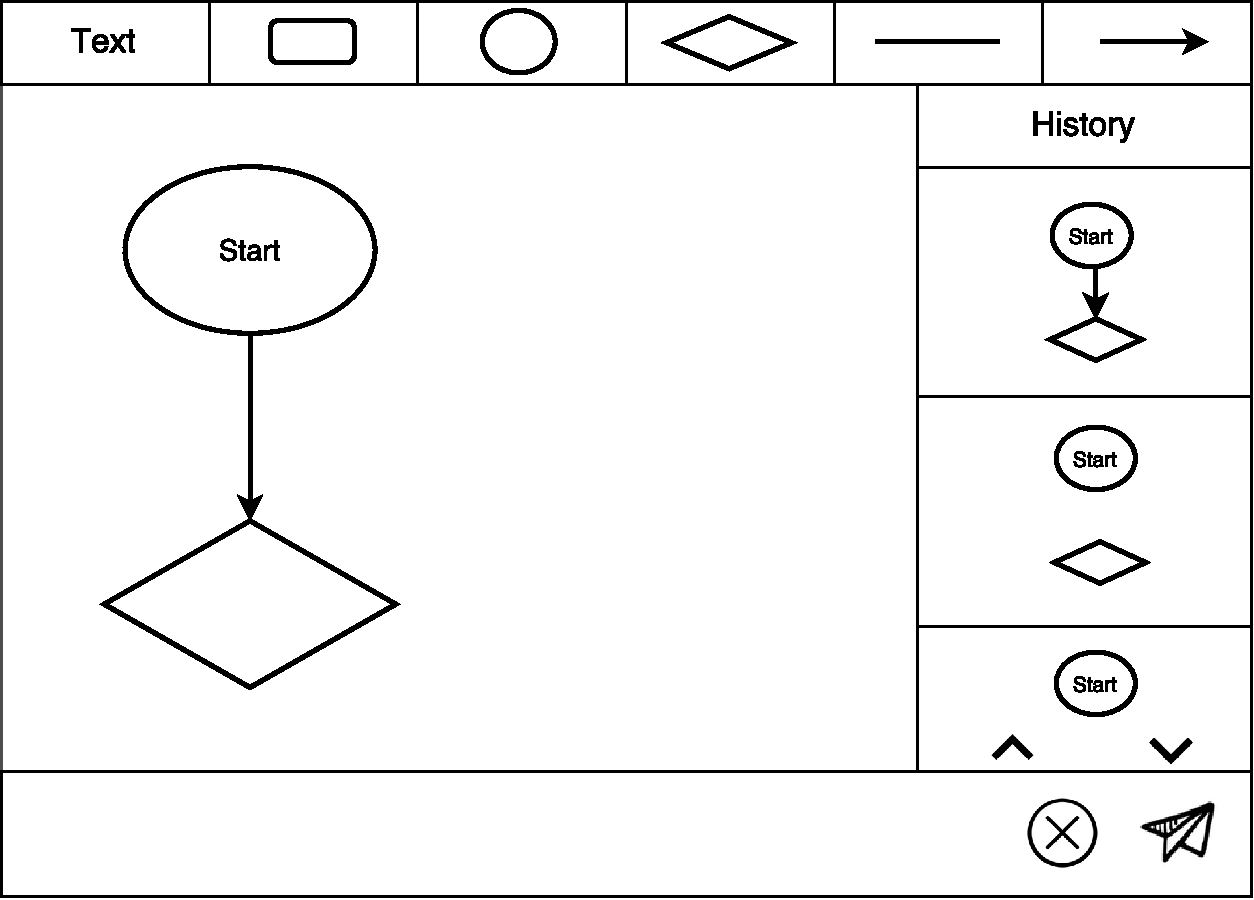
\includegraphics[width=0.8\textwidth]{Figures/mockup/editor.pdf}
  \caption{Drawing editor with drawing history}
\end{figure}
% Mockups history list, undo, redo


\end{enumerate}


\subsection{Realtime}
How to ease the approach of content acquisition and improve the interactivity for arousing enthusiasm of students, is also a key point while designing the discuss system. So two major realtime functionalities are featured as follow: 

% Auto Ordering of Questions / Answers
% Sidebar notifications!

\begin{enumerate}
\item
\textbf{Realtime Question List}: Without requesting the question list initiatively, all new questions posted by other users will be pushed to user automatically. The user doesn't have to concern himself with acquisition of the new content anymore.

\begin{figure}[!htbp]
  \centering
    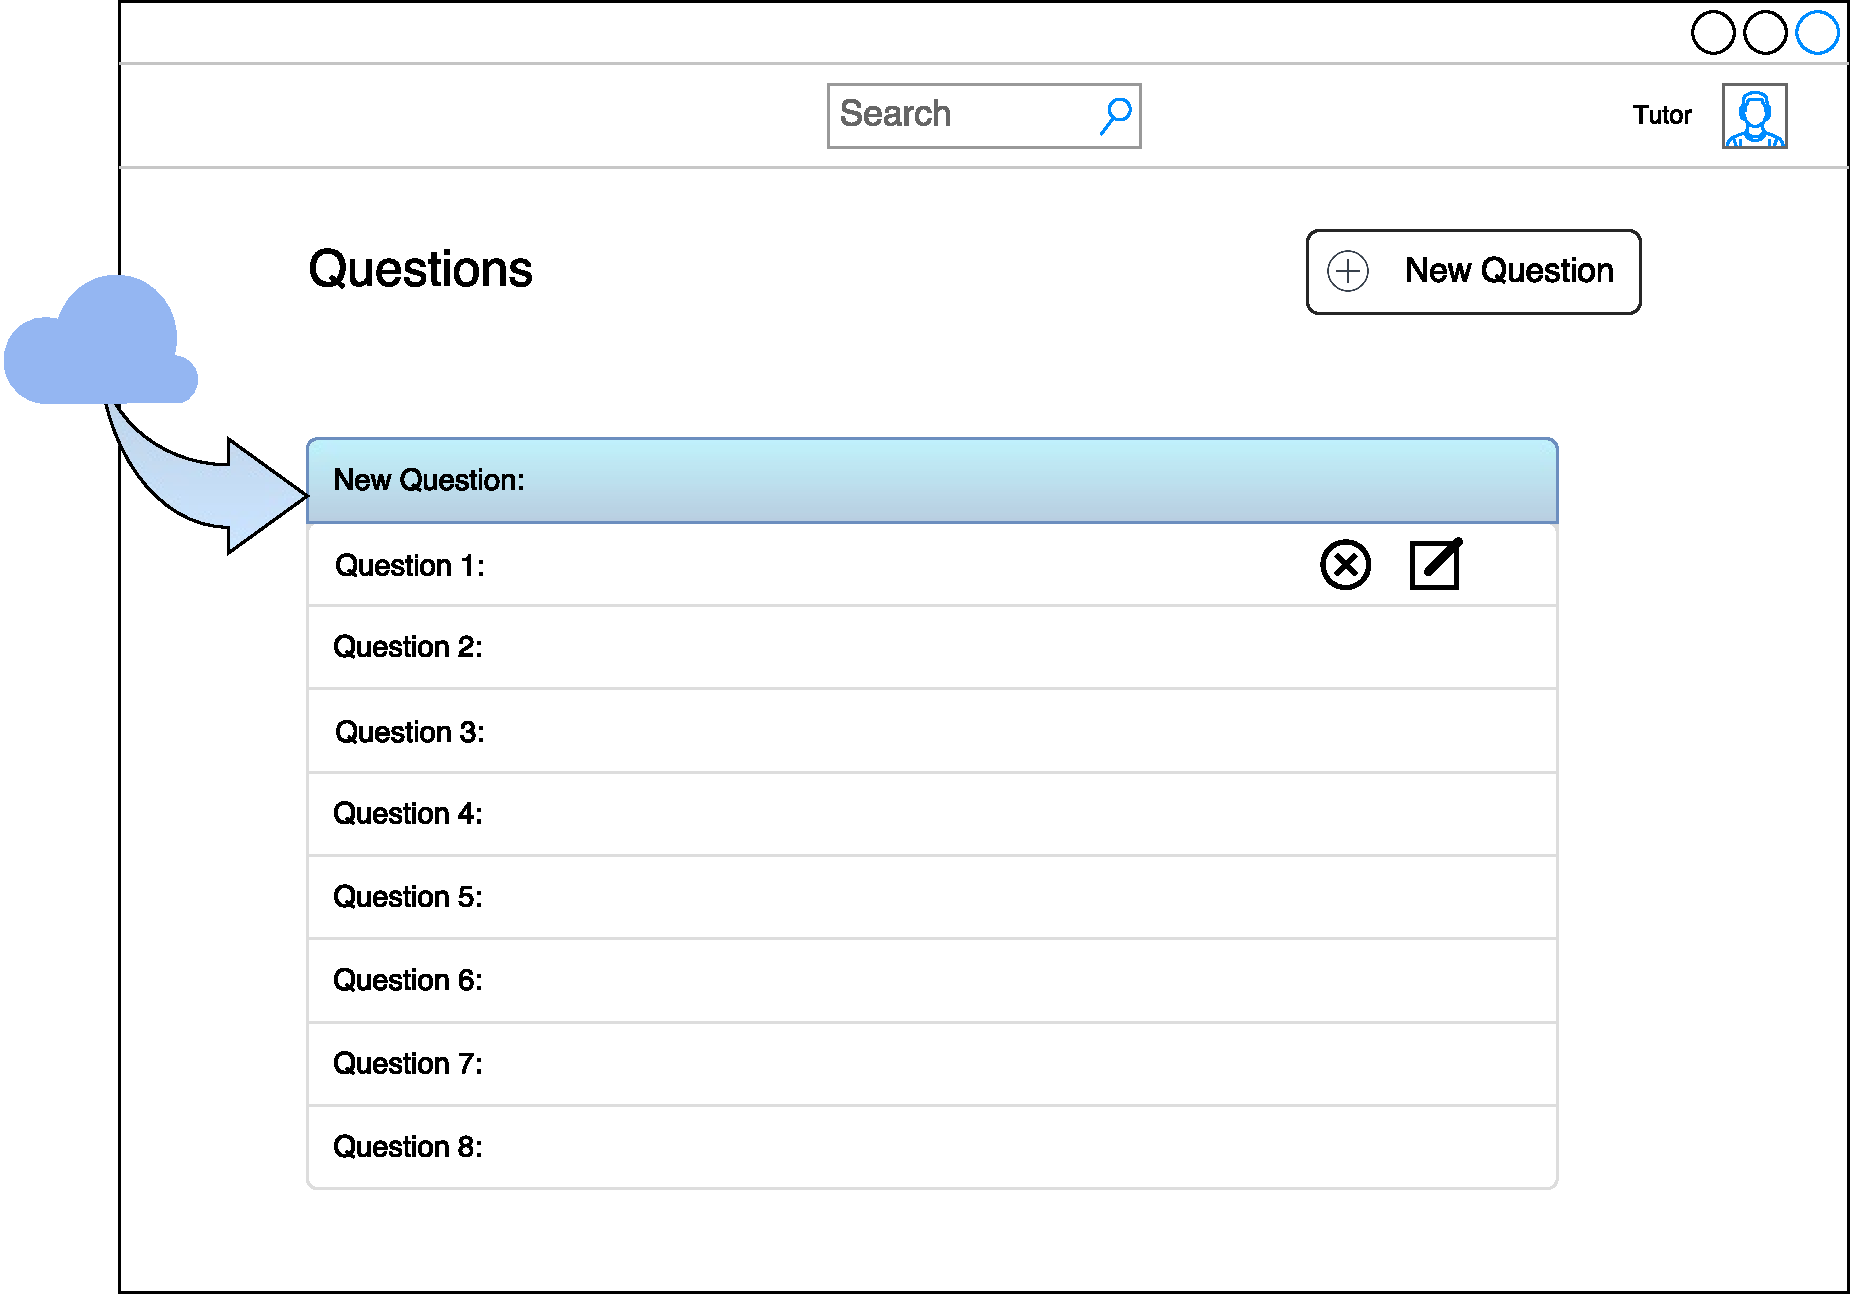
\includegraphics[width=0.8\textwidth]{Figures/mockup/question-notify.pdf}
  \caption{Notify with new question automatically}
\end{figure}

\item
\textbf{Realtime Answer Ordering}: Without refreshing the page, the answers will be re-ordered as new vote action is triggered.

\begin{figure}[!htbp]
  \centering
    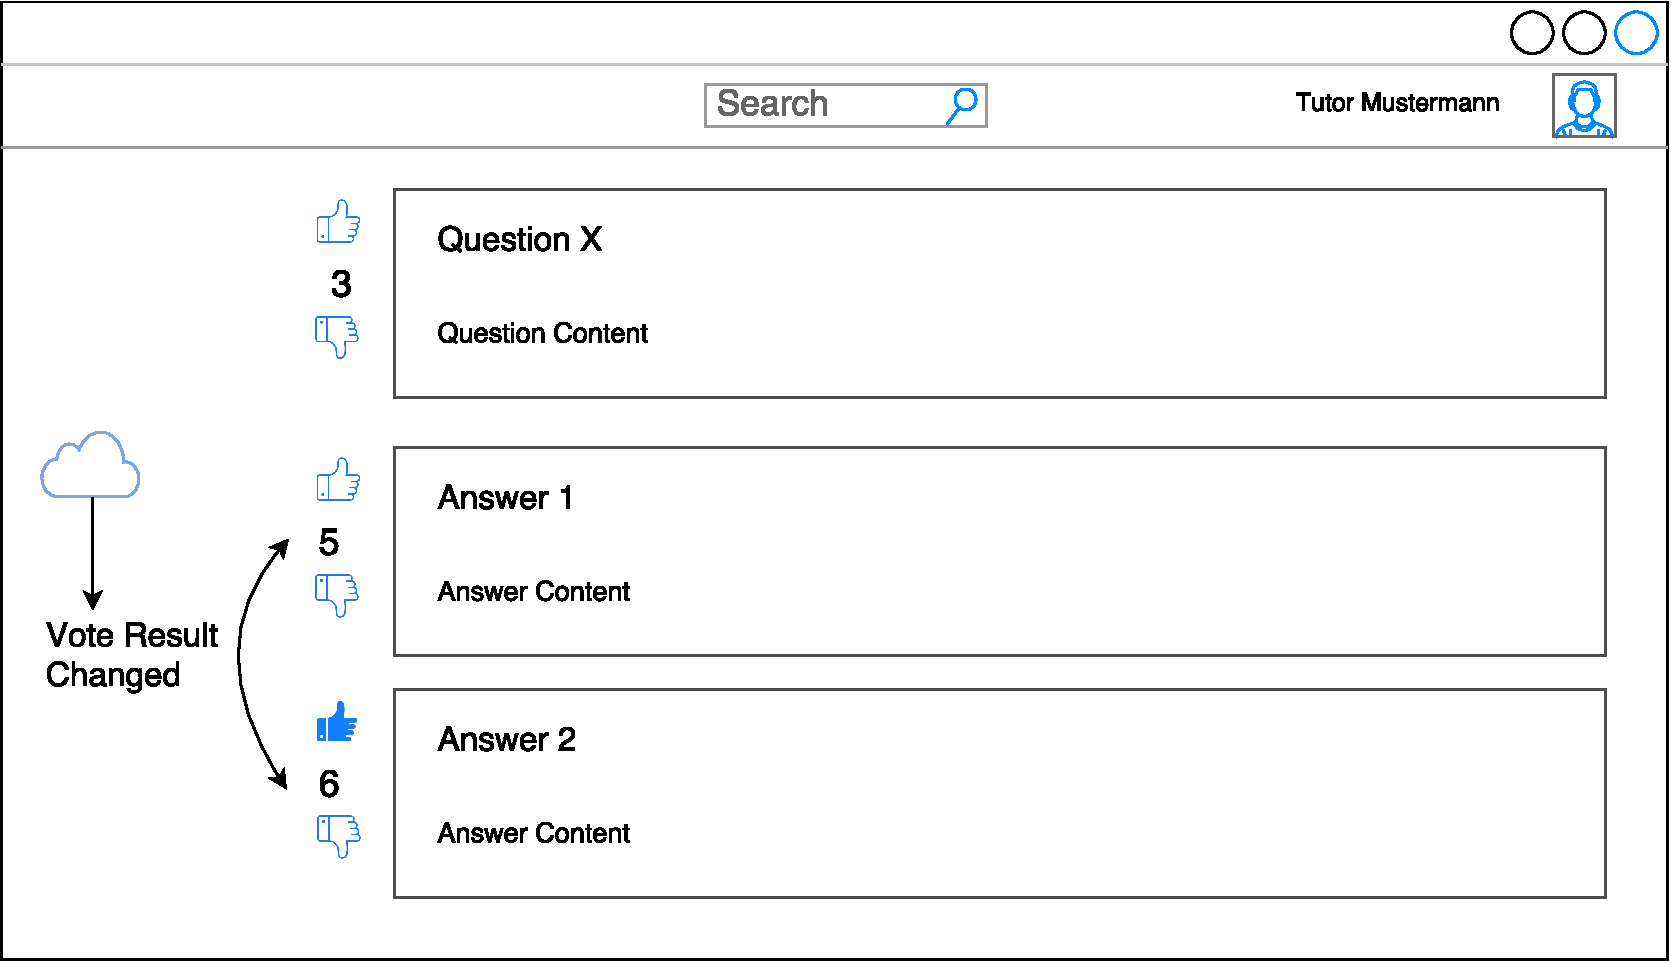
\includegraphics[width=0.8\textwidth]{Figures/mockup/votechange.pdf}
  \caption{Anto re-order answer if vote contributions changed}
\end{figure}
% Mockups Upvote/downvote, arrange of answer.


\end{enumerate}


% WHat's the difficulties. How we compare and solve it?
\chapter{Conception}
!!! In this chapter a conception of the discuss system including both client and server side will be described. In the first section, all the essential requirements are presented. After that, the general conception or workflow of the application will be proposed. The more concrete details and definitions of the conception will also be outlined. In addition, the focal points behind the conception and the proper solutions of the difficulties will be illustrated.


\section{Aims and Objectives}\label{sec:aims}
Before starting to concept the graphical discuss system, it's necessary to analyse requirements and objectives behind the origin motivation in the first place. It should be defined at first, what kind of functionalities should be achieved and how the system behaves.

\subsection{Basic Functionalities}

As a graphical discuss system for the educational purpose, the system should contain basic functionalities on the prototype  of a forum which could be organized by classes. So class management, question management and answer management are the tree essential parameters to be designed at the start.

\subsubsection{Course Management}

Each question should have a certain domain of its content, so the questions are organized by classes initially. The features of course management should be:

\begin{enumerate}
\item
\textbf{Create Course}: The user who is identified as a tutor is able to create course and maintain the course he created. While creating the course, the tutor can define the name of the course and upload an image as a background of the course for better recognization. In addition, concret description of the course could also be added to the description area.

\begin{figure}[!htbp]
  \caption{placeholder}
  \centering
    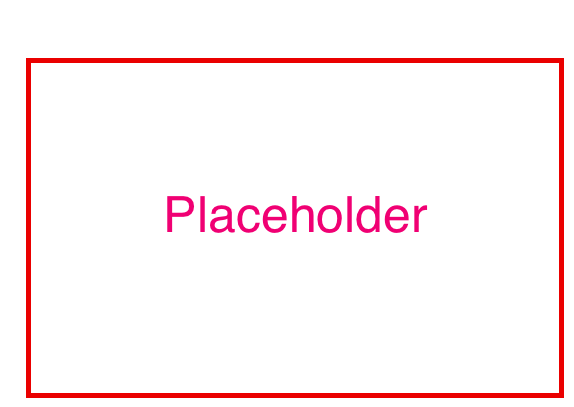
\includegraphics[width=0.6\textwidth]{Figures/placeholder.png}
  \label{fig:placeholder}
\end{figure}

% Mockups create, upload, description

\item
\textbf{Search Course}: After a course is created, a corresponding unique identifier code for the course will be generated at the same time. The students are able to find the course through the identifier code.

\begin{figure}[!htbp]
  \caption{placeholder}
  \centering
    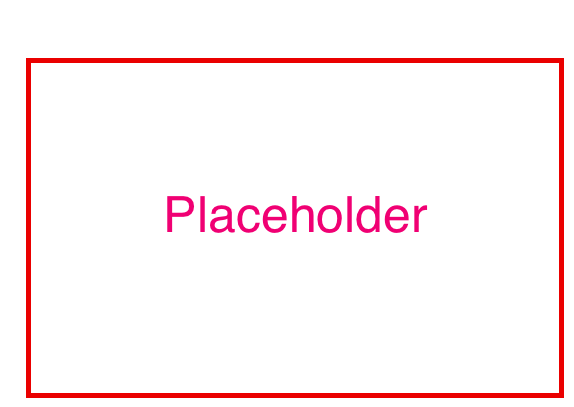
\includegraphics[width=0.6\textwidth]{Figures/placeholder.png}
  \label{fig:placeholder}
\end{figure}
% Mockups code, search

\item
\textbf{Favor Course}: If a student is interest to a certain course, he is capable to add the course to his favor list so that it's easy to find and access the course he liked later.

\begin{figure}[!htbp]
  \caption{placeholder}
  \centering
    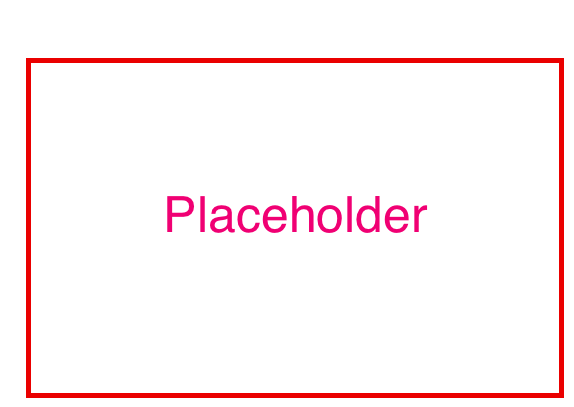
\includegraphics[width=0.6\textwidth]{Figures/placeholder.png}
  \label{fig:placeholder}
\end{figure}
% Mockups fav button, fav list.

\end{enumerate}

\subsubsection{Question Management}

\begin{enumerate}
\item
\textbf{Submit/Edit/Withdraw Question}: The student who has confusion with the teaching content can submit his own question with detailed description in a certain course. The user is also permitted to edit the question if he want to add more precise informations or modify the unclarity he made to the question. Withdrawing of his own question is also possible, but only when there're no contributes made to the question.

\begin{figure}[!htbp]
  \caption{placeholder}
  \centering
    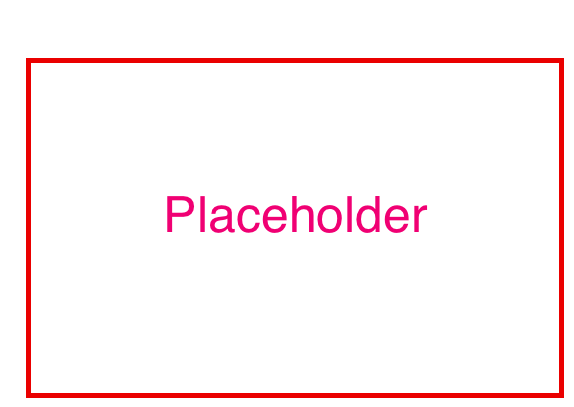
\includegraphics[width=0.6\textwidth]{Figures/placeholder.png}
  \label{fig:placeholder}
\end{figure}
% Mockups submit/Edit, withdraw

\item
\textbf{Upvote/Downvote Question}: An assessment of a question is decisive for building a better community with high-quality contents. So the user is able to upvote or downvote of a question and determine if the question is helpful for other members in the community or not.

\begin{figure}[!htbp]
  \caption{placeholder}
  \centering
    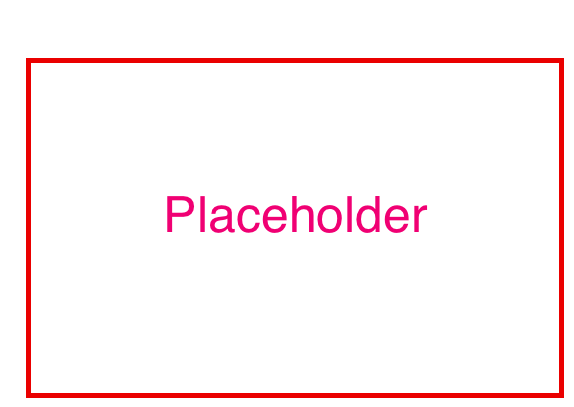
\includegraphics[width=0.6\textwidth]{Figures/placeholder.png}
  \label{fig:placeholder}
\end{figure}
% Mockups Upvote/downvote.

\item
\textbf{Favor Question}: If the student consider the question as a helpful and useful content and want to review this question in the future, he can favor the question and locate it in a certain list.

\begin{figure}[!htbp]
  \caption{placeholder}
  \centering
    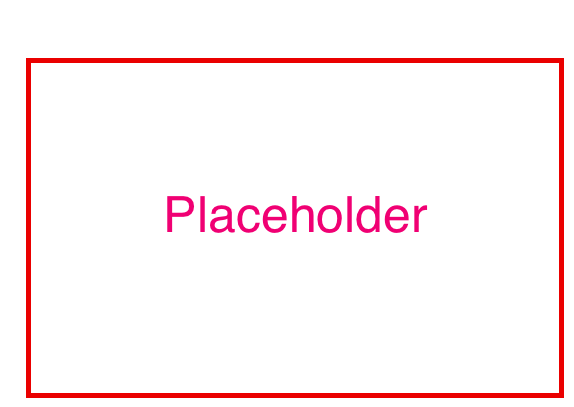
\includegraphics[width=0.6\textwidth]{Figures/placeholder.png}
  \label{fig:placeholder}
\end{figure}
% Mockups Fav, fav list

\item
\textbf{Accept Answer}: The owner of the question has the right to accept the most useful answer in his opion which will be shown up at the top of the answer list.

\begin{figure}[!htbp]
  \caption{placeholder}
  \centering
    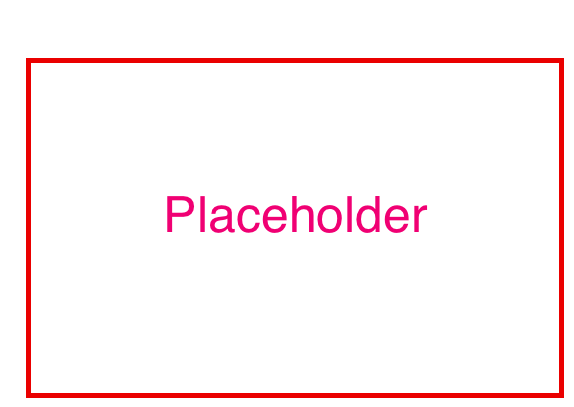
\includegraphics[width=0.6\textwidth]{Figures/placeholder.png}
  \label{fig:placeholder}
\end{figure}
% Mockups Accept, Top.

\end{enumerate}

\subsubsection{Answer Management}

\begin{enumerate}
\item
\textbf{Submit/Modify/Remove Answer}: User who has experence with the question can submit his answer to the question. After the submission, the modification or removal of the user's own question is possible.

\begin{figure}[!htbp]
  \caption{placeholder}
  \centering
    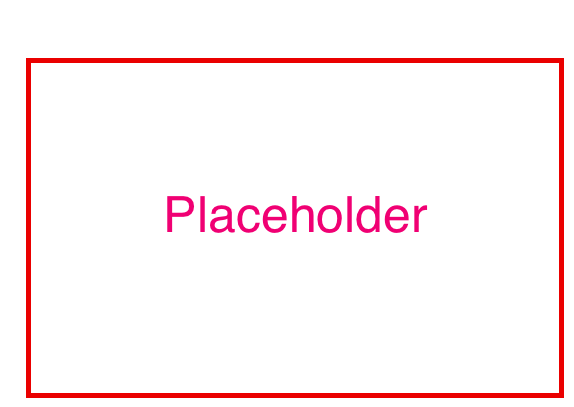
\includegraphics[width=0.6\textwidth]{Figures/placeholder.png}
  \label{fig:placeholder}
\end{figure}
% Mockups submit, withdraw

\item
\textbf{Upvote/Downvote Answer}: As mentioned above in section of question functionality, a similar idea of assessment should also be applied to answers. Answer with higher vote will be listed at first.

\begin{figure}[!htbp]
  \caption{placeholder}
  \centering
    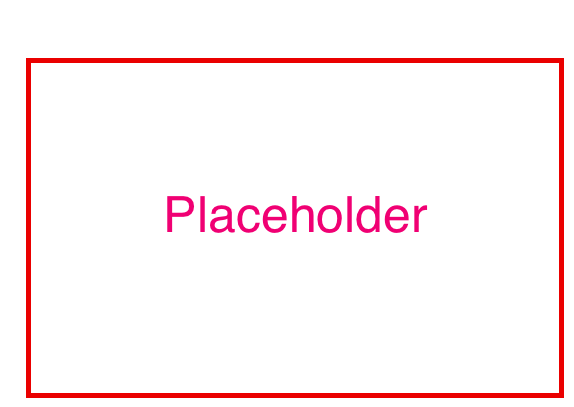
\includegraphics[width=0.6\textwidth]{Figures/placeholder.png}
  \label{fig:placeholder}
\end{figure}
% Mockups Upvote/downvote, arrange of answer.

\item
\textbf{Quote Answer}: Answers are able to be quoted so that the user can supplement informations on the top of original post or point out the deficiency of the contribute.

\begin{figure}[!htbp]
  \caption{placeholder}
  \centering
    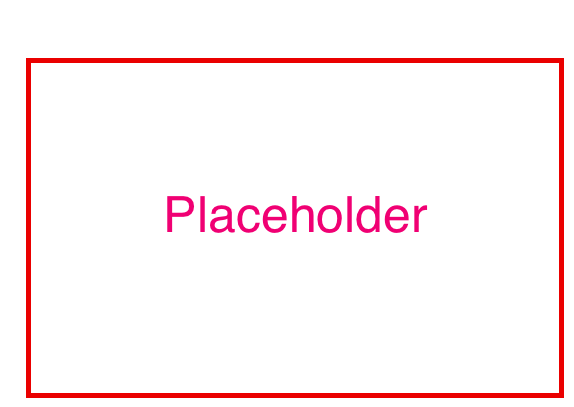
\includegraphics[width=0.6\textwidth]{Figures/placeholder.png}
  \label{fig:placeholder}
\end{figure}
% Mockups Fav, fav list

\end{enumerate}


\subsection{High Interativity}
Building with the basic functionalities is far not enough. To fit the system for educational purpose and improve the interactivity for arousing enthusiasm of students, a drawing tool and realtime functionality should be intergrated into the system.

\subsubsection{Drawing Tool}
Normally, some of the thoughts can't be simply expressed by textual description, so a drawing tool should be designed to enables the user to compose not only text but also different components such like rectangle, circle, line and so on, which helps the user to express his question more precisely.
The ideal drawing tool should have following features:

\begin{enumerate}
\item
\textbf{Draw Diverse Components}: Not only text but also diverse components could be drawn while posting a contribution. Styling of a component such as size tuning, color changing is also the essential, which will helps emphasize the important part the user expressing.

\begin{figure}[!htbp]
  \caption{placeholder}
  \centering
    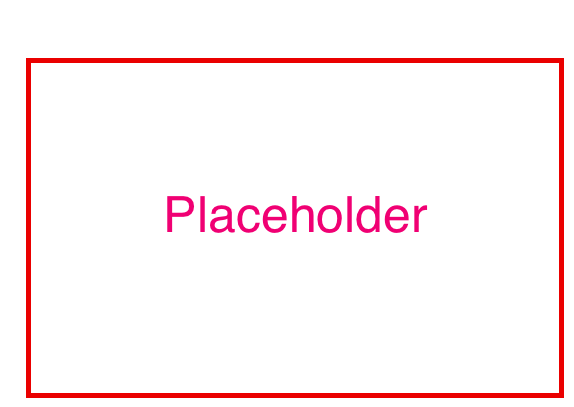
\includegraphics[width=0.6\textwidth]{Figures/placeholder.png}
  \label{fig:placeholder}
\end{figure}
% Mockups draw components, styling

\item
\textbf{Drawing History}: During drawing, the user might make mistakes or change mind after placing a component or text. So a history list of drawing actions bundled with undo and redo functionalities will dramatically improve the usability of drawing process.

\begin{figure}[!htbp]
  \caption{placeholder}
  \centering
    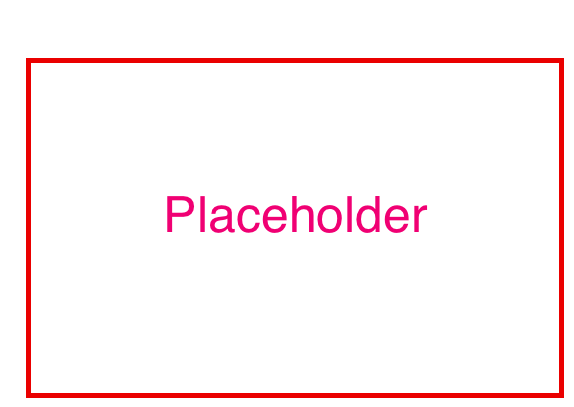
\includegraphics[width=0.6\textwidth]{Figures/placeholder.png}
  \label{fig:placeholder}
\end{figure}
% Mockups history list, undo, redo


\end{enumerate}


\subsubsection{Realtime}
How to ease the approach of content acquisition and improve the interactivity for arousing enthusiasm of students, is also a key point while designing the discuss system. So two major realtime functionalities are featured as follow: 

% Auto Ordering of Questions / Answers
% Sidebar notifications!

\begin{enumerate}
\item
\textbf{Realtime Question List}: Without requesting the question list initiatively, all new questions posted by other users will be pushed to user automatically. The user doesn't have to concern himself with acquisition of the new content anymore.

\begin{figure}[!htbp]
  \caption{placeholder}
  \centering
    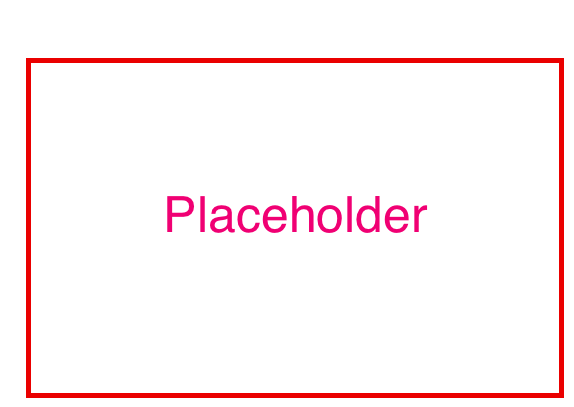
\includegraphics[width=0.6\textwidth]{Figures/placeholder.png}
  \label{fig:placeholder}
\end{figure}
% Mockups submit, withdraw

\item
\textbf{Realtime Answer Ordering}: Without refreshing the page, the answers will be re-ordered as new vote action is triggered.

\begin{figure}[!htbp]
  \caption{placeholder}
  \centering
    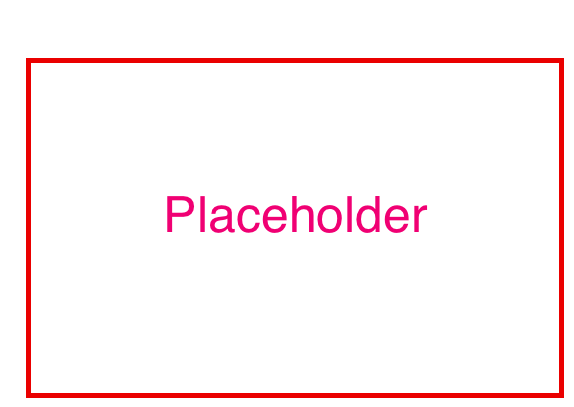
\includegraphics[width=0.6\textwidth]{Figures/placeholder.png}
  \label{fig:placeholder}
\end{figure}
% Mockups Upvote/downvote, arrange of answer.


\end{enumerate}

\section{General Concept}
Before the whole conception of the system, a general conceptual architecture of the system should be defined initially. In order to help understanding how the system works, the primary data flow between different domains will also be described.

\subsection{Architecture} \label{sec:concept-general-architecture}
According to the analysis result of Single-Page-App in chapter \ref{chapter:state-of-the-art}, and considering the demand on high interactivity and ubiquity as well as scalability in the graphical discuss system, leveraging SPA architecture will benefit a lot and accelerate the implementation of the system. 

In general, the entire system will be divided into two parts: namely client and server-side. Each side is basically full independent to the other and has its own responsibility. 

\begin{enumerate}
\item
\textbf{Client}: The client is totally responsible for initial view rendering and view re-rendering as the view model changes. 
\item
\textbf{Server}: The server is in charge of core business logic, data processing, data persistence and also provides the client interfaces for data acquisition.
\end{enumerate}

% General Architecture of System including Server(data persistence with db) + Client(has multiple views, one template engine, re-render with new data.)
\begin{figure}[!htbp]
  \centering
    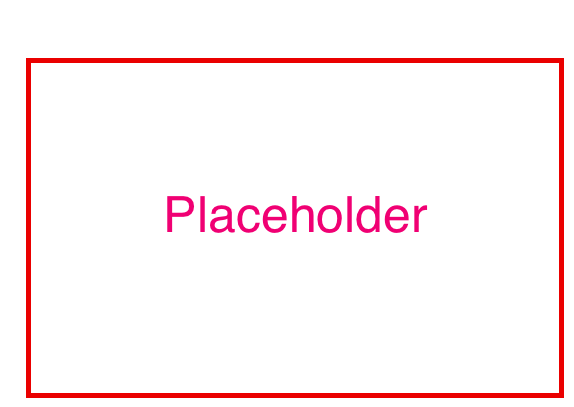
\includegraphics[width=0.6\textwidth]{Figures/placeholder.png}
  \caption{placeholder}
  \label{fig:general-architecture-concept}
\end{figure}

General architecture of the system is described in figure \ref{fig:general-architecture-concept}, the only bridge between the client and server-side is data transmission service. Complete separation of both sides will also accelerate the development flow in implementation phase. Once the protocol of data transmission services is fully confirmed and defined, development of each side is able to performed parallelly. Furthermore, technical choices on both sides are more flexible. Both sides are able to apply the technologies which fit them most without coupling to each other, the only thing they should obey is to follow the protocol of data transmission.

\subsection{Communication} \label{subsection:concept-general-communication}
As mentioned above in section \ref{sec:concept-general-architecture}, data communication is the only coupling factor in the general architecture. In this system, there exist two different type of protocols: standard HTTP using REST architecture and WebSocket with persistent connection. Each data transmission protocol has its own responsibility and usage scenario.

\begin{enumerate}
\item
\textbf{HTTP with REST architecture}: Data which is requested initiatively is transferred over HTTP. The HTTP connection will be closed as soon as the data is successfully transferred.
\item
\textbf{WebSocket with persistent connection}: Reactive data with realtime need is transferred over WebSocket. After the persistent connection is established, client are able to receive the data at the first moment as the state of data is updated. 
\end{enumerate}

% Pic broadcast to multiple clients with different events. engine to rerender
\begin{figure}[!htbp]
  \centering
    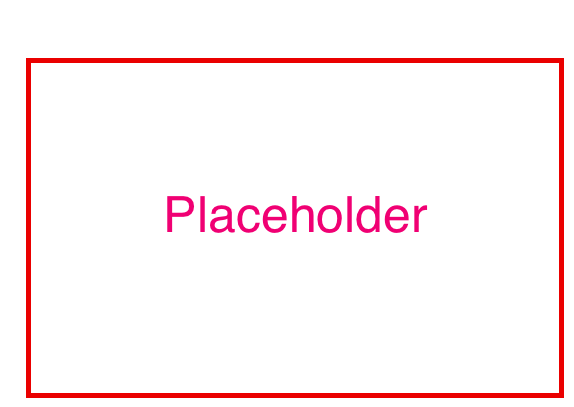
\includegraphics[width=0.6\textwidth]{Figures/placeholder.png}
  \caption{placeholder}
  \label{fig:general-data-communication-concept}
\end{figure}

As figure \ref{fig:general-data-communication-concept} shows, in case data for view model is acquired from server despite transferred over HTTP or WebSocket, the views are re-rendered. Comparing with HTTP, the specialty of data acquisition over WebSocket is: a listener for specific resource with unified process of data processing and automatic view re-rendering will be created.
\section{Data Definitions}\label{sec:data-concept}
In this section, data modelling of the system including definitions of data domain, data fields for each domain, and relation between domains will be performed in the first place. In the following subsection, APIs corresponding to related operations on data models will be assigned.

\subsection{General Data Model}


\subsubsection{ Data Domain }
In general, data in the system could be divided into 4 primary domains:

\begin{itemize}
\item
\textbf{User}: personal information as well as user identifier for accessing the system.
\item
\textbf{Course}: a container with own course information as well as collection of questions classified to this context.
\item
\textbf{Question}:  data with information of questions submitted by users.
\item
\textbf{Answer}: data with information of answers, also has graphical data within the data model.

\end{itemize}

Users are able to assess the contributions made by other users and mark it as useful or useless, which will affect the contributions' oder priority while rendering the views. Voters should also be aware of what kind of vote he has marked to the contribution. Therefore, additional 2 data models \textbf{VoteAnswer} and \textbf{VoteQuestion} should also be considered. 

The relation between domains is illustrated in the following figure \ref{ata-domain-relation}. Each data modal has an unique identifier, which is referenced in another data model when they have a connection. 

\begin{figure}[!htbp]
  \centering
    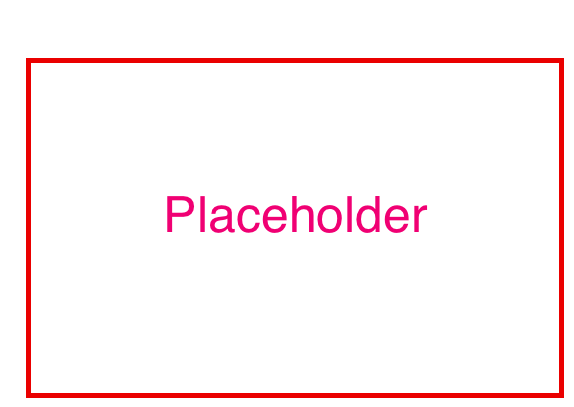
\includegraphics[width=0.6\textwidth]{Figures/placeholder.png}
  \caption{placeholder}
  \label{fig:data-domain-relation}
\end{figure}
% relation pic
% Belonging!!! User->Course->Question->Answers!
% PowerDesigner - Tool!


\subsubsection{ Data Fields }

More detailed definition and description of fields in each data model should be made for a better understanding of the structure as well as behaviour of a data model. Tabel \ref{data-field-table} describes key fields of general domains.


\begin{table}[]
\centering
\begin{tabularx}{\textwidth}{@{}llX@{}}
\toprule
Domain                    & Field           & Description                                                                                    \\ \midrule
\multirow{4}{*}{User}     & email           & unique identifier of an user for authentification, also as contact way to user.                \\
                          & password        & string for user authentication to prove identity or access approval                            \\
                          & username        & user identifier shown to other users                                                           \\
                          & isTutor         & flag which determines if the user is a student or tutor                                        \\ \midrule
\multirow{4}{*}{Course}   & name            & name of the course                                                                             \\
                          & desc            & description of the course                                                                      \\
                          & creator         & id of the user(tutor) who created this course                                                  \\
                          & code            & unique code for quick search purpose which is generated automatically as the course is created \\ \midrule
\multirow{5}{*}{Question} & title           & title of the question                                                                          \\
                          & content         & content of the question                                                                        \\
                          & course          & id of the the course to which the question belongs                                             \\
                          & vote            & vote count of the question                                                                     \\
                          & creator         & id of the user who submitted this question                                                     \\ \midrule
\multirow{5}{*}{Answer}   & content         & content of the answer                                                                          \\
                          & question        & id of the question for which the answer is made                                                \\
                          & quoted          & id of the original question which is quoted                                                    \\
                          & vote            & vote count of the answer                                                                       \\
                          & creator         & id of the submitter                                                                            \\ \midrule
\multirow{3}{*}{Vote}     & type            & enum values of up-voting or down-voting actions                                                \\
                          & handler         & id of the hander                                                                               \\
                          & question/answer & id of the question/answer to which the vote action is applied                                  \\ \midrule
\end{tabularx}
\caption{Fields for Each Data Domain}
\label{table:data-field-table}
\end{table}


\subsection{RESTful API Definitions}

As mentioned in section xxx, RESTful architecture is a an excellent technical choice for data transferring. Because of its simplicity and clear semantic description of HTTP methods comparing to other protocols such like SOAP, it will dramatically simplify and clarify our data transmission services. 

\subsubsection{ Mapping of HTTP methods to data model behaviour }
The data model defined above can directly map to the definition of resources in RESTful. The HTTP methods on each resource domain can also represent the data model behaviours, \textbf{\textit{User Model}} is taken as an example: 
\begin{table}[!htbp]
\centering
\begin{tabularx}{\textwidth}{@{}lX@{}}
\toprule
Method        & {Operation of data model collection }                            \\ \midrule
GET           & {Query and return a specific user from user model collection.}   \\
POST          & {Create a new user entry and insert into user model collection.} \\
PUT           & {Update a specific user in user model collection.}               \\
DELETE        & {Delete a specific user in user model collection.}               \\ \bottomrule
\end{tabularx}
\caption{HTTP methods on User resource}
\label{table:http-method-on-user-resource}
\end{table}

In table \ref{http-method-on-user-resource}, resource entry in persistent storage can be executed with specific action while requesting resource URI through different HTTP methods. A semantic description of connection between \gls{CRUD} and HTTP methods on RESTful will make the data transmission services more understandable and unified.

\subsubsection{ General RESTful API Definitions }

Requesting a specific resource can only succeed through its \gls{URI}, through which the client and server-side could connect to each other actually. Therefore, a definition of APIs which describes \gls{URI} of the resources and its functional responsibility should be proposed in the first place.


\begin{itemize}
\item
\textbf{User Authentication}: the major actions of user authentication include signup, login, logout. To protect the user information, POST method which doesn't expose information via the URL, is highly recommended.

\begin{table}[!htbp]
\centering
\begin{tabularx}{\textwidth}{@{}llX@{}}
\toprule
URI          & Method & Description                                                  \\ \midrule
/auth/login  & POST   & User login action, request with login information.           \\
/auth/signup & POST   & User signup action, request with registration information.   \\
/auth/logout & GET    & User logout action, no data submission is needed.            \\ \bottomrule
\end{tabularx}
\caption{User Auth APIs}
\label{table:user-auth-apis}
\end{table}

\item
\textbf{Courses}: acquisition of courses and new submission of a course is possible. In addition, \gls{CRUD} operations on a specific course should also be achieved through a single URI with various HTTP methods.

\begin{table}[!htbp]
\centering

\begin{tabularx}{\textwidth}{@{}llX@{}}
\toprule
URI                 & Method         & Description                                                                                                          \\ \midrule
/courses            & GET/POST       & request the whole collection of courses; create course with data submitted \\
/courses/:courseId & GET/PUT/DELETE & request, modify, remove specific entry of course                                                                     \\ \bottomrule
\end{tabularx}
\caption{Course Resource APIs}
\label{table:course-resource-apis}
\end{table}

\item
\textbf{Questions}: in a real sense question resource is attached to course resource. According to the best practise of RESTful API design [reference xxx], question resource could be touched under course URI, \textit{/courses/:courseId/questions/:questionId}. But in the real world, question resource has its own collection, and \textit{questionId} is the unique identifier, through which a specific question entry could be selected without using  
\textit{courseId}. So an optimized conception is simply using \textit{/questions} as URI instead. And pass \textit{courseId} as a query parameter while requesting collection of question entries under a specific course. 
\begin{table}[!htbp]
\centering

\begin{tabularx}{\textwidth}{@{}llX@{}}
\toprule
URI                                   & Method         & Description                                                                                                                                                 \\ \midrule
/questions?courseId=:id               & GET/POST       & request the whole collection of questions belonging to a specific course; create question under a specific course \\
/questions/:id                & GET/PUT/DELETE & request, modify, remove specific entry of question                                                                                                          \\
/questions/:id/vote/:type      & POST          & vote actions with different vote types applied to specific question  \\ \bottomrule
\end{tabularx}
\caption{Question Resource APIs}
\label{table:question-resource-apis}
\end{table}


\item
\textbf{Answers}: the general API design of answer is totally same as the approach applied in question resource. A independent API for voting functionality should also be designed. And multiple possibilities of vote types could also be passed through the API.

\begin{table}[!htbp]
\centering

\begin{tabularx}{\textwidth}{@{}llX@{}}
\toprule
URI                                 & Method         & Description                                                                                                                                                 \\ \midrule
/answers?questionId=:id             & GET/POST       & request the whole collection of answers belonging to a specific question; create answer under a specific question\\
/answers/:id                        & GET/PUT/DELETE & request, modify, remove specific entry of answer                                                                                                            \\
/answers/:id/vote/:type             & POST           & vote actions with different vote types applied to specific answer                                                                                           \\ \bottomrule
\end{tabularx}
\caption{Answer Resource APIs}
\label{table:answer-resources-apis}
\end{table}

\end{itemize}

Once all APIs with different HTTP methods are defined, a more concrete data structure over the APIs between two sides should be promised and confirmed. By following defined APIs and promised data structure, developments on both client and server-side could be executed parallelly.

\subsection{WebSocket Definitions} \label{subsection:websocket-definition-data-concept}

As the requirements defined in section \ref{sec:aims}, users could be informed as new question is posted or the order of answers with rating priority changes. Basically, only two different types of listeners are needed in this case: one for listening to the new questions under a specific class and one for responsive order of answers under a specific question. With WebSocket, URI should also be defined as an identifier for the persistent connection between client and server. And different events within a connection of one URI should also be designed. Table \ref{table:websocket-def} defines these two WebSocket specifications.

\begin{table}[!htbp]
\centering
\begin{tabularx}{\textwidth}{@{}llX@{}}
\toprule
URI                       & Event           & Response                           \\ \midrule
/ws/courses/            & questions-changed       &  data of new question posted by others \\
/ws/questions/          & answers-changed      &  data of answers in new order          \\ \bottomrule
\end{tabularx}
\caption{Answer Resource APIs}
\label{table:websocket-def}
\end{table}


\section{Graphical Data Serialization}\label{sec:graphical-data-serialization-concept}
% conventrion problem
% redo, undo: hooks, history
% dawing tool!

Graphical content is the most efficient and intuitive way to deliver the explanation of an answer to other users comparing with pure textual content. In this section, Choices for graphical technologies on the Web will be analysed in order to figure out which is the ideal and fit the graphical discussion system most. 


\subsection{Canvas versus SVG}



\subsection{Converting Canvas Data }



\subsection{Drawing Tool}

% problem Quote - then Fabric.js
% Problem How to combine rich text editor with graphical?
\section{Real-Time Demand}\label{sec:realtime-concept}
% when realtime?
% problem: efficiency, not open all socket for all resource
% only by demand! open/close socket room dynamically.

Realtime communication as mentioned in subsection \ref{subsection:concept-general-communication} are used for reactive data, which requires WebSocket for establishing persistent connections to enable the bi-directional communication between client and server.


All users are able to subscribe arbitrary course for new submission of a question as well as arbitrary question for updated order of answers, and server could also push realtime data to those users who has subscribed the resource with specific identifier. However, only two WebSocket services: \textit{/ws/courses} and \textit{/ws/questions} are defined as the entry points according to the definition in subsection \ref{subsection:websocket-definition-data-concept}. The approach how the server broadcast data precisely to the users who subscribe resources they require should be resolved.

A feasible solution is that the server maintains a list of user ids and resource ids subscribed by user. Afterwards, as a specific resource is updated, the server can get all users who has subscribed this resource from the maintained list using the resource's identifier.

\begin{figure}[!htbp]
  \centering
    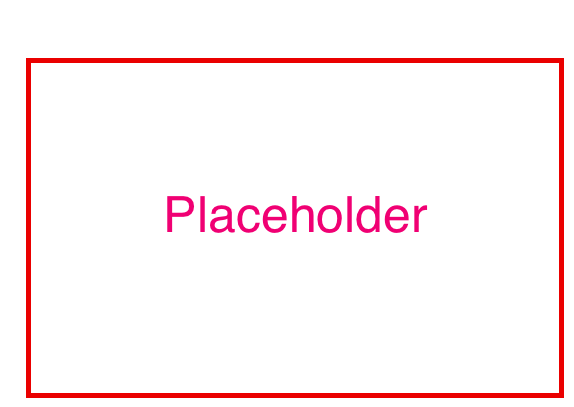
\includegraphics[width=0.6\textwidth]{Figures/placeholder.png}
  \caption{placeholder}
  \label{fig:websocket-connection-sequence-concept}
\end{figure}

%zhuangtaitu! status diagram!!! connected -> emit id to listen -> a list of mapping maintained by server.

Figure \ref{fig:websocket-connection-sequence-concept} represents the whole workflow of establishing the connection over WebSocket. In the first place, the server starts listening for requests over WebSocket protocol with specific URI. Then the user start a connection to server for subscribing the resource he requires. As soon as the connection is successfully established, the client will emit the resource id to the server side, and resource id from client will be mapped to the user id in a list maintained by the server.

After that, the server has the information of which user has subscribed which resource, and is able to emit realtime data precisely.
% problem - then dispatcher
% Roles?

% \section{Challenges}
% 
\subsection{Graphical Data Convertion}
% % conventrion problem
% redo, undo: hooks, history
% dawing tool!

Graphical content is the most efficient and intuitive way to deliver the explanation of an answer to other users comparing with pure textual content. In this section, Choices for graphical technologies on the Web will be analysed in order to figure out which is the ideal and fit the graphical discussion system most. 


\subsection{Canvas versus SVG}



\subsection{Converting Canvas Data }



\subsection{Drawing Tool}

% problem Quote - then Fabric.js
% Problem How to combine rich text editor with graphical?
\subsection{Real-Time Demand}
% % when realtime?
% problem: efficiency, not open all socket for all resource
% only by demand! open/close socket room dynamically.

Realtime communication as mentioned in subsection \ref{subsection:concept-general-communication} are used for reactive data, which requires WebSocket for establishing persistent connections to enable the bi-directional communication between client and server.


All users are able to subscribe arbitrary course for new submission of a question as well as arbitrary question for updated order of answers, and server could also push realtime data to those users who has subscribed the resource with specific identifier. However, only two WebSocket services: \textit{/ws/courses} and \textit{/ws/questions} are defined as the entry points according to the definition in subsection \ref{subsection:websocket-definition-data-concept}. The approach how the server broadcast data precisely to the users who subscribe resources they require should be resolved.

A feasible solution is that the server maintains a list of user ids and resource ids subscribed by user. Afterwards, as a specific resource is updated, the server can get all users who has subscribed this resource from the maintained list using the resource's identifier.

\begin{figure}[!htbp]
  \centering
    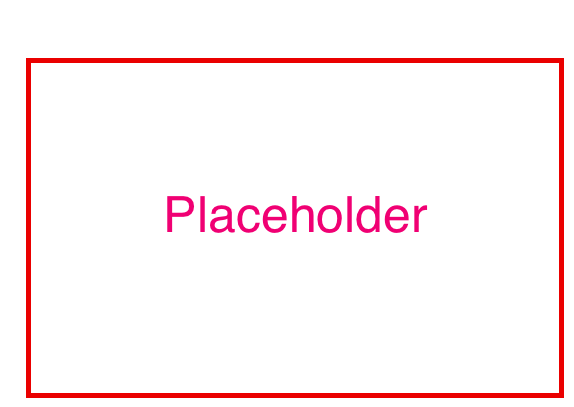
\includegraphics[width=0.6\textwidth]{Figures/placeholder.png}
  \caption{placeholder}
  \label{fig:websocket-connection-sequence-concept}
\end{figure}

%zhuangtaitu! status diagram!!! connected -> emit id to listen -> a list of mapping maintained by server.

Figure \ref{fig:websocket-connection-sequence-concept} represents the whole workflow of establishing the connection over WebSocket. In the first place, the server starts listening for requests over WebSocket protocol with specific URI. Then the user start a connection to server for subscribing the resource he requires. As soon as the connection is successfully established, the client will emit the resource id to the server side, and resource id from client will be mapped to the user id in a list maintained by the server.

After that, the server has the information of which user has subscribed which resource, and is able to emit realtime data precisely.
% problem - then dispatcher
% Roles?

\section{Conclusion}


Conclusion!

Conclusion!

Conclusion!

Conclusion!

Conclusion!

Conclusion!

Conclusion!

Conclusion!


Conclusion!

Conclusion!

Conclusion!

Conclusion!


Conclusion!

Conclusion!

Conclusion!

Conclusion!





\chapter{Implementation}
In this chapter, an prototype of graphical discussion system will be created and make use of the previously developed approach as a "proof of concept". Firstly, ... the application domain will be presented and also foreshadow the prototype funtionality. Afterwards, ... the development itself will take place, highlighting and documenting best practices in the subsequent sections.


\section{General}
On the whole, the implementation can be divided into two parts: client and server. Since they are fully separated, each part is considered and structured as a independent project. The implementation on client side is basically data fetching and template rendering, while data persistence and core business logic is implemented on the server side.  For convenience, the graphical discuss system is named \textbf{"Graphicuss"}, which stands for graphical plus discuss.


\subsection{Platform and Framework}
To achieve a better performance of view rendering on client side running in browser, React.js\footnote{https://facebook.github.io/react/ - accessed 10 July 2016} is taken as the front-end framework. Componentization, the main philosophy of ReactJS, also helps organize the views and view model logics. On the server side, ExpressJS\footnote{http://expressjs.com/ - accessed 12 July 2016} as a web framework is adopted for its efficiency and productivity of building RESTFul APIs.

Since both client and server projects are primarily implemented in JavaScript, NodeJS\footnote{https://nodejs.org/ - accessed 12 July 2016} is the single development environment for either project implementation or project management on both sides.

\subsubsection{File Structure}

To have a basic understanding of whole project including the server side and client side, a file structure of the project Graphicuss is listed in figure \ref{fig:overview-file-structure}:

\begin{itemize}
\item 
  \textbf{client/}: independent front-end project built on top of ReactJS
\item
  \textbf{server/}: independent back-end project implemented by using ExpressJS
\item
  \textbf{dist/}: compiled back-end project integrated with compiled and compressed static view files from front-end project
\item 
  \textbf{node\_modules/}: source of referenced third party libraries
\item 
  \textbf{package.json}: definition of third party libraries for client and server side
\item 
  \textbf{webpack.config.json}: config of specific behaviours in automated development or building process
\end{itemize}

\begin{figure}[!htbp]
\centering
\begin{forest}
  for tree={
    font=\ttfamily,
    grow'=0,
    child anchor=west,
    parent anchor=south,
    anchor=west,
    calign=first,
    edge path={
      \noexpand\path [draw, \forestoption{edge}]
      (!u.south west) +(7.5pt,0) |- node[fill,inner sep=1.25pt] {} (.child anchor)\forestoption{edge label};
    },
    before typesetting nodes={
      if n=1
        {insert before={[,phantom]}}
        {}
    },
    fit=band,
    before computing xy={l=15pt},
  }
[Graphicuss
  [client/]
  [server/]
  [dist/]
  [node\_modules/]
  [package.json]
  [webpack.config.js]
]
\end{forest}
\caption{Overview of Graphicuss' file structure}
\label{fig:overview-file-structure}
\end{figure}


\subsubsection{Module Management}

NodeJS provides native module management which is called \textit{npm}\footnote{https://www.npmjs.com - accessed 12 July 2016}. Third party libraries, which are published in the official remote repository, can be installed conveniently by only using npm's command line. There is also a list of names of all modules and dependencies in the file \textit{package.json}. Installing all dependencies and modules can be simply achieved by using only one command line \textit{npm install}, which will significantly ease the setting up process of the project freshly on a new machine.

\subsection{Architecture}

An architectural overview of Graphicuss is illustrated in figure \ref{fig:general-arch-imp}.

\begin{figure}[!htbp]
  \centering
    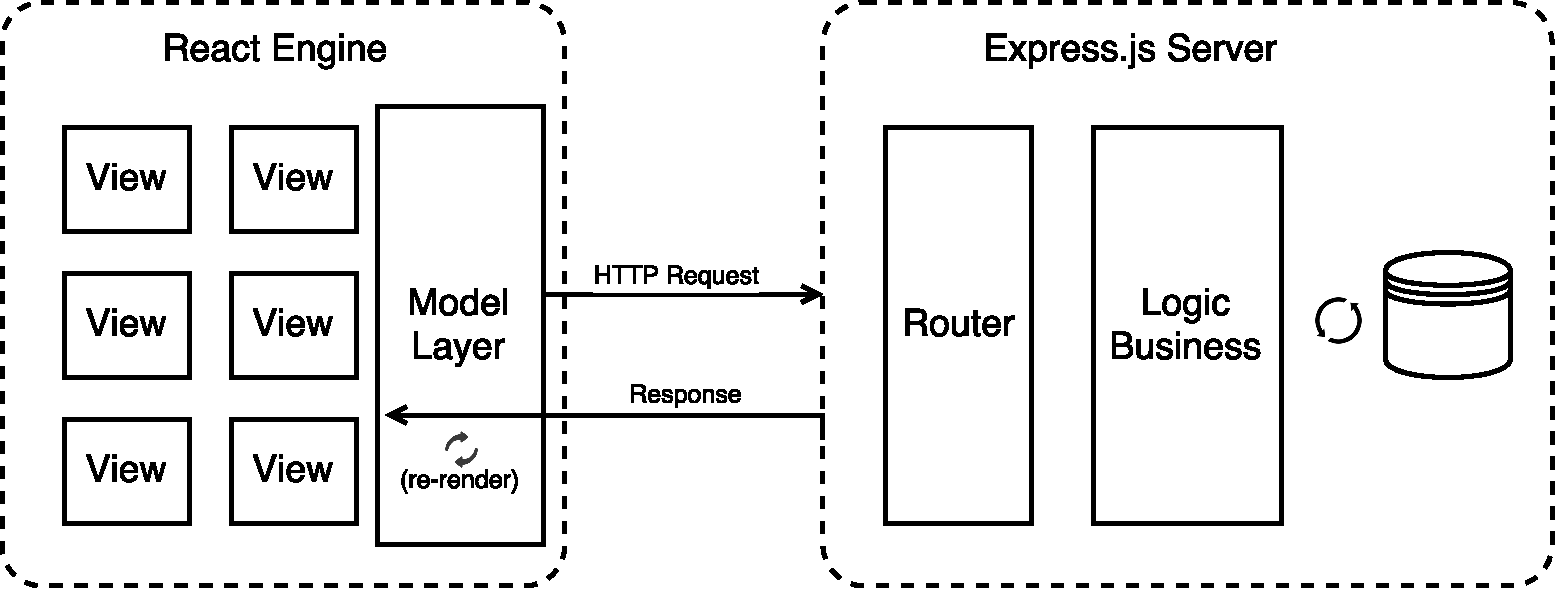
\includegraphics[width=1\textwidth]{Figures/imp-general-arch.pdf}
  \caption{General architecture}
  \label{fig:general-arch-imp}
\end{figure}
% Big Pic! Client with xuxian circle domain + React Engine -> Router in Express -> logic business + Database -> return 
While the client starts requesting a specific URL for data from the server, a HTTP connection will be established. The server program receives the HTTP request and forwards it to its router, in which rules for matching URLs have been pre-defined. By analysing headers of HTTP request, router will check if the request matches any pre-defined rules.

Not only the URL but also the parameters passed by client, for example the identifier of a resource, could also be extracted from HTTP headers. Server runs correlate business logics according to the rule of matched URL and executes operations of databases for data persistence. Afterwards, results are returned from server.

As soon as the data is successfully returned, the HTTP connection will be closed. The client processes data acquired from server, and represents it by re-rendering views. So far, a entire request over HTTP is accomplished.

\subsection{Automatization}
To accelerate the developing as well as building process of the project, a automatization tool called \textit{Webpack}\footnote{https://webpack.github.io/ - accessed 13 July 2016} is used. 

Webpack is a tool which could analyse the dependencies of the project and bundle modules with the app. In addition, it can also do tasks like compressing JavaScript codes to reduce the size of the client app, or compiling modern JavaScript as well as CSS codes to achieve the compatibility for old browsers.

\subsubsection{Automated Development Process}
To make the development of client app independent, it will start a dev server on its own for development purpose. However the dev server started by client app and the actual server are running on different ports. Which means that the communication between them will cause CORS problem.

CORS means, a resource makes a cross-origin HTTP request when it requests a resource from a different domain than the one which the first resource itself serves. For security reasons, browsers restrict cross-origin HTTP requests initiated from within scripts. \cite{CORS}

Through configuring the dev server started by Webpack, a proxy could established to forward request to the actual back-end server. As figure \ref{fig:proxy-server-imp} shows, the client is able now to request APIs under the same domain, and requests will go though the dev server, after that they are forwarded to the actual server.

\begin{figure}[!htbp]
  \centering
    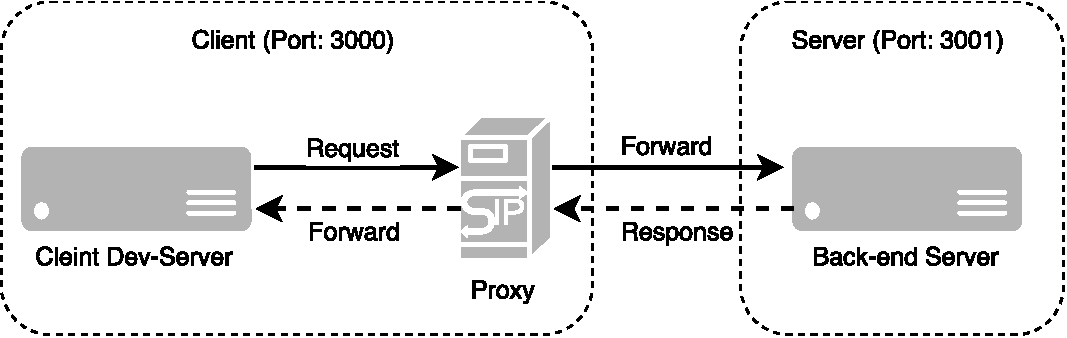
\includegraphics[width=1\textwidth]{Figures/imp-proxy-server.pdf}
  \caption{Proxy for client development server}
  \label{fig:proxy-server-imp}
\end{figure}
% Dev Process, in development(dev server, proxy) + building)


\subsubsection{Automated Building Process}

For the client app, multiple tasks are executed during the building process by using Webpack: transforming modern JavaScript code, pre-processing the modern CSS code and bundling the static files. All these tasks will significantly reduce the size of client app and also improve the compatibility of the app.

Webpack also helps accelerate the building process by defining various automated building tasks. It will bundle all dependencies with the server app and client app. After processing on both sides, the final output of the files will be extracted into the \textit{dist} directory mentioned in \ref{fig:overview-file-structure}, which is now ready for deploying and serving. The whole building process is represented in figure \ref{fig:automated-building-imp}.

\begin{figure}[!htbp]
  \centering
    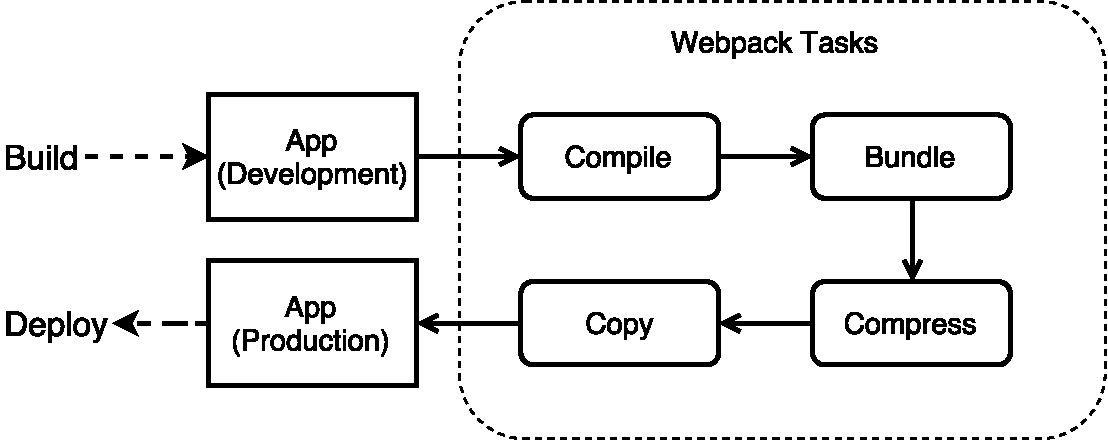
\includegraphics[width=1\textwidth]{Figures/imp-automated-building.pdf}
  \caption{Automated building process with Webpack}
  \label{fig:automated-building-imp}
\end{figure}
% Building Process, a->b->c->d xuxian kuang, Webpack compile, bundle, compress -> copy file to dist -> ready for deploy

\subsection{Storage Structure} \label{subsec:storage-structure-imp}
In section \ref{sec:data-concept}, data domains and fields of data domains  have already been defined. 

For all persistence storage of data on the server side a MongoDB\footnote{https://www.mongodb.com/ - accessed 13 July 2016} database is used.  In figure \ref{fig:data-model-table-imp}, more concrete definition of data model table is defined. MongoDB is a non-SQL database, which uses document oriented storage and JSON style data model. That will make it easy to implement as well as scale data models. In addition, An \gls{ORM} framework called Mongoose\footnote{http://mongoosejs.com/ - accessed 13 July 2016} is also applied to the implementation, which encapsulates the native database operations of MongoDB. With help of the \gls{ORM} framework, definition of schema and query on database will be quite simple. 

% Description othe the table?

\begin{figure}[!htbp]
  \centering
    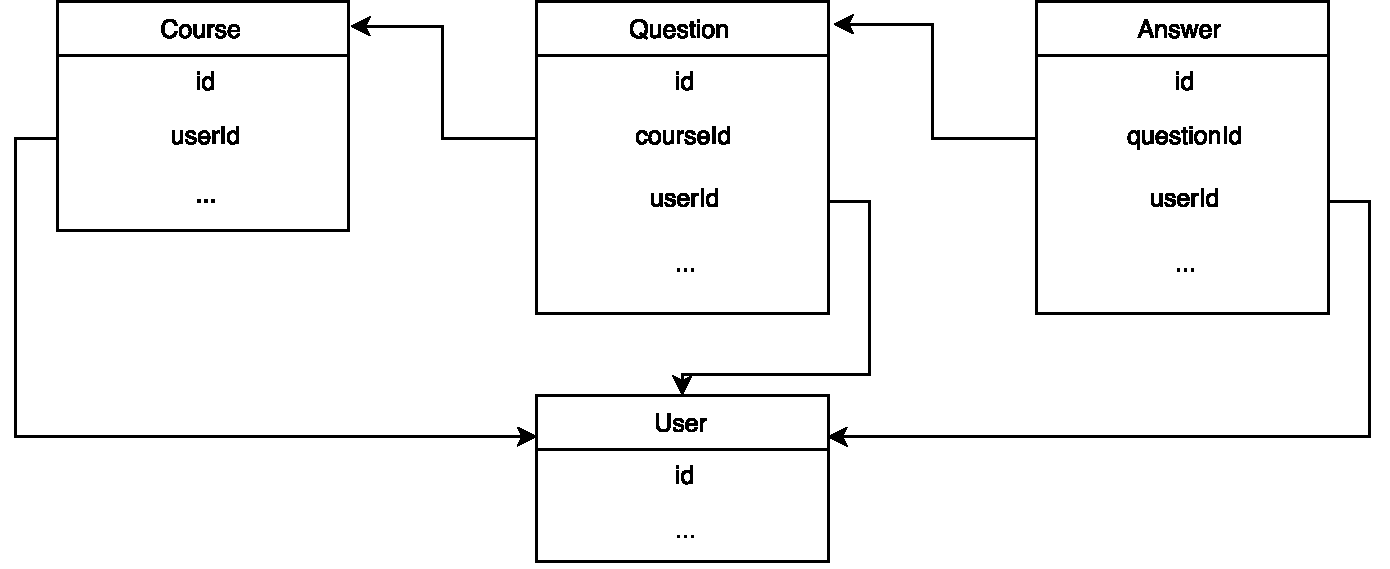
\includegraphics[width=1\textwidth]{Figures/concept-data-domain-relation.pdf}
  \caption{Table of data model}
  \label{fig:data-model-table-imp}
\end{figure}
% Whole Concret Data Model Table

 % File Structure, Data Design, Workflow(automated)

\section{Server of Graphicuss}
This section gives the explanation of architectural pattern and more detailed implementation of the server side. 

% Architecture MV, , JWT for Auth, Websocket Dispatcher, Resource Listening?

\subsection{Architecture}

\subsubsection{MVC Pattern and Project Structure}
To separate the different layers of model, view and controller, \gls{MVC} pattern is used as the basic pattern of the architecture. In the model layer, all data model related concerns such as data shema definitions, data model validation as well as database operations are defined. And Controllers contain the core domain logics, process the data from model layer, and pass the result to view layer.

Since the templates are rendered on the client side, the view layer is just simply stripped. Therefore, basically the controllers response processed data to client side directly without rendering it to views. Figure \ref{fig:server-file-structure-imp} shows the overview of the server's  file structure which is featured with MVC pattern.

\begin{figure}[!htbp]
\centering
\begin{forest}
  for tree={
    font=\ttfamily,
    grow'=0,
    child anchor=west,
    parent anchor=south,
    anchor=west,
    calign=first,
    edge path={
      \noexpand\path [draw, \forestoption{edge}]
      (!u.south west) +(7.5pt,0) |- node[fill,inner sep=1.25pt] {} (.child anchor)\forestoption{edge label};
    },
    before typesetting nodes={
      if n=1
        {insert before={[,phantom]}}
        {}
    },
    fit=band,
    before computing xy={l=15pt},
  }
[server
  [config/
    [index.js]
    [routes.js]
  ]
  [models/]
  [controllers/]
  [index.js]
  [...]
]
\end{forest}
\caption{Overview of server app's file structure}
\label{fig:server-file-structure-imp}
\end{figure}


\begin{enumerate}
\item 
  \textbf{index.js}: the entry point of the whole server app. It will create a server instance and set up configurations for the server. In addition, a connection from server instance to database will be established. After all configurations are done, the server instance will start listening port and waiting for the requests from client.
\item
  \textbf{config/index.js}: config as well as constants for the server. It persists \textit{apiConfig} for example the common prefix of API URL and version of the API. And config for database including the database URL will be defined here as well. In addition, keys for encryption are also stored in the config file.
\item
  \textbf{config/routes.js}: rules for URL matching. All URL matching rules are defined in this file. Controllers are referenced here and a dispatcher for router will be instantiated. If any request meets the defined rule, the request will be forward to a correlative controller. 
\item
  \textbf{controllers/*}: controllers for processing specific requests.
\item 
  \textbf{models/*}: data model definitions. Files under this directory are organized by different data domain.
\end{enumerate}


\subsubsection{Achitecture of Server}

The figure \ref{fig:server-arch-imp} illustrates an overview of the server's architecture. 

\begin{figure}[!htbp]
  \centering
    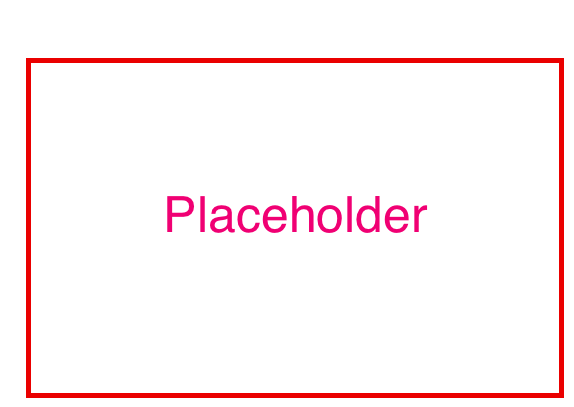
\includegraphics[width=0.6\textwidth]{Figures/placeholder.png}
  \caption{placeholder}
  \label{fig:server-arch-imp}
\end{figure}
% process of request to be handeled. index.js -> create server isntance -> connect to database. routes -> different controllers -> different models

\subsection{Data Schema Definition}
% Architecture MV, , JWT for Auth, Websocket Dispatcher, Resource Listening?

\section{Client of Graphicuss}



\subsection{Architecture}
For the implementation of the client application, \textit{React.js} which aims to solve the challenges involved when developing web application with complex user interfaces, is applied. To have a better concept of how Graphicuss's client application is implemented, an overview of the file structure is listed in the figure \ref{fig:client-file-structure-imp}.

\subsubsection{Project Structure}
\begin{figure}[!htbp]
\centering
\begin{forest}
  for tree={
    font=\ttfamily,
    grow'=0,
    child anchor=west,
    parent anchor=south,
    anchor=west,
    calign=first,
    edge path={
      \noexpand\path [draw, \forestoption{edge}]
      (!u.south west) +(7.5pt,0) |- node[fill,inner sep=1.25pt] {} (.child anchor)\forestoption{edge label};
    },
    before typesetting nodes={
      if n=1
        {insert before={[,phantom]}}
        {}
    },
    fit=band,
    before computing xy={l=15pt},
  }
[client
  [components/
    [AppBar/
      [index.js]
      [style.css]
    ]
    [...]
  ]
  [containers/]
  [models/]
  [utils/]
  [index.js]
  [index.html]
  [...]
]
\end{forest}
\caption{Overview of client app's file structure}
\label{fig:client-file-structure-imp}
\end{figure}

\begin{itemize}
  \item 
  \textbf{components/}: all components are defined by extending basic \textit{React.Compoent}. Each custom component has an \textit{index.js}, which processes the logics of view rendering and applies view model to the template. \textit{style.css} defines the CSS style of the HTML DOMs within a component.
  \item 
  \textbf{containers/}: containers are compositions of components.
  \item 
  \textbf{models/}: in model directory, data models for the components are defined. In addition, the definition of APIs and processing after data acquisition  also take place here.
  \item 
  \textbf{index.js \& index.html}: \textit{index.js} is the entry point of the app, which will instantiate the React instance and render the views into a specific DOM defined  in \textit{index.html}
\end{itemize}


\subsubsection{Achitecture of Client}

An overview of the client application's architecture is revealed in figure \ref{fig:client-arch-imp}. 

\begin{figure}[!htbp]
  \centering
    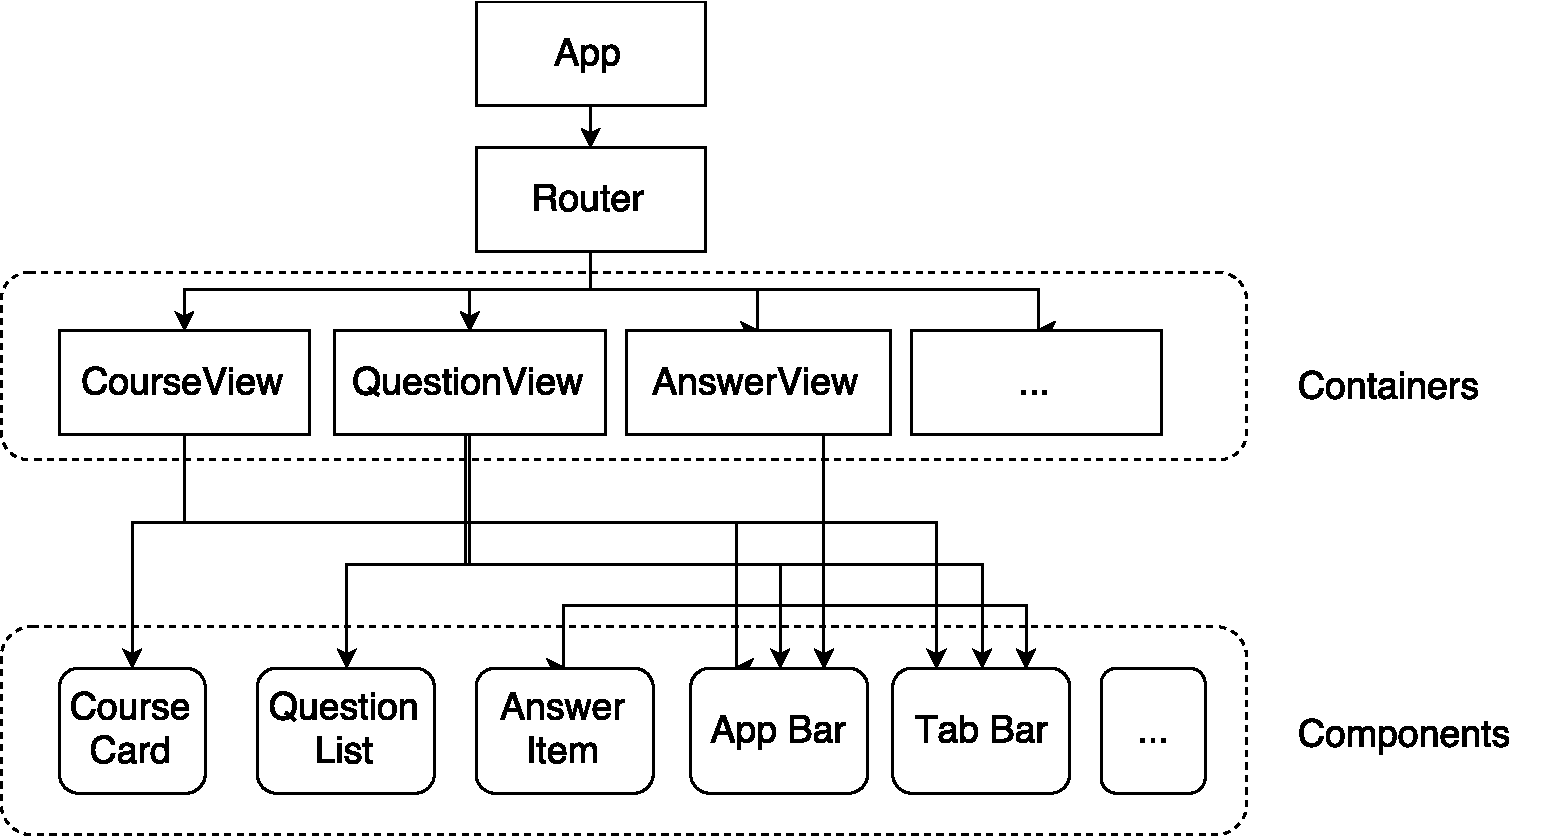
\includegraphics[width=1\textwidth]{Figures/imp-client-arch.pdf}
  \caption{Overview of client architecture}
  \label{fig:client-arch-imp}
\end{figure}
% client arch, App -> router containes rotes -> different container -> components(Compisition... for containers!) xuxian for layer (App, router, container, components)

In the React application, \textit{Router} is also regarded  as a component, in which different matching rules of URL are defined. If the URL requested by user is matched, a correlate view will be rendered according to the definition of routes. Code list \ref{list:router-client-imp} shows the implementation of defining a \textit{Router} component.

\begin{lstlisting}[language=HTML, caption=Router in client app , label={list:router-client-imp}]
<Router history={history}>
  <Route path="/" component={App}>
    <Route path="auth" component={AuthView} />
    <Route path="courses" component={CoursesView} />
    <Route path="courses/:courseId" component={QuestionsView} />
    <Route path="questions/:questionId" component={AnswersView} />
  </Route>
</Router>
\end{lstlisting}

Containers such like \textit{CourseView}, \textit{QuestionsView} or \textit{AnswersView} are compositions of components in fact. The way how component acquires view model is that the parent component pass values to its child component by defining the properties of the child component. So the data flow starts from the root component and goes through every child components. 

How to manage the data flow and control the rendering behaviour will be discussed later in the sub section \ref{subsection:data-flow-react-imp}.


\subsection{Composition of Components}

\subsubsection{React Component}

Defining a new \textit{Component} with React.js must extent the \textit{React.Component} class and implement the \textit{render()} function, which will be called when the component is instantiated. Afterwards, the template as well as the composition of components are rendered to plain HTML.  A simplfied example of building a \textit{CourseView} component is represented in code list \ref{list:course-view-render-imp}.

\begin{lstlisting}[language=HTML, caption=Rendering \textit{CourseView} with multiple \textit{CourseCard} components , label={list:course-view-render-imp}]
class CoursesView extends React.Component {
  render() {
    const courses = this.props.courses
    return (
      <div>
        {
          courses.map( (course) =>
            <CourseCard course={course} key={course._id}></CourseCard>
          )
        }
      </div>
    ); 
  }
}
\end{lstlisting}

As mentioned above, the parent components pass data through as the properties of child components. Within the \textit{CoursesView}, \textit{courses} could be read from its properties which is defined while \textit{CourseView} is composed. In the \textit{render()} function of \textit{CourseView}, \textit{courses} are traversed and each single \textit{course} will be passed into the \textit{CourseCard} as its property. Which means, as \textit{CourseView} is rendered, all \textit{CourseCard} components within it will also call their own \textit{render()} functions with the data model passed in. Data flows from top to bottom, likewise, views are rendered from parent to children components.

\subsubsection{Composition}
\textit{Components} are the core of React. All each view and its view model of the client application is represented as a React \text{Component}. And the whole client app is actually a composition of React components. An example of \textit{CoursesView} is taken in figure \ref{fig:course-view-composition-imp}.

\begin{figure}[!htbp]
  \centering
    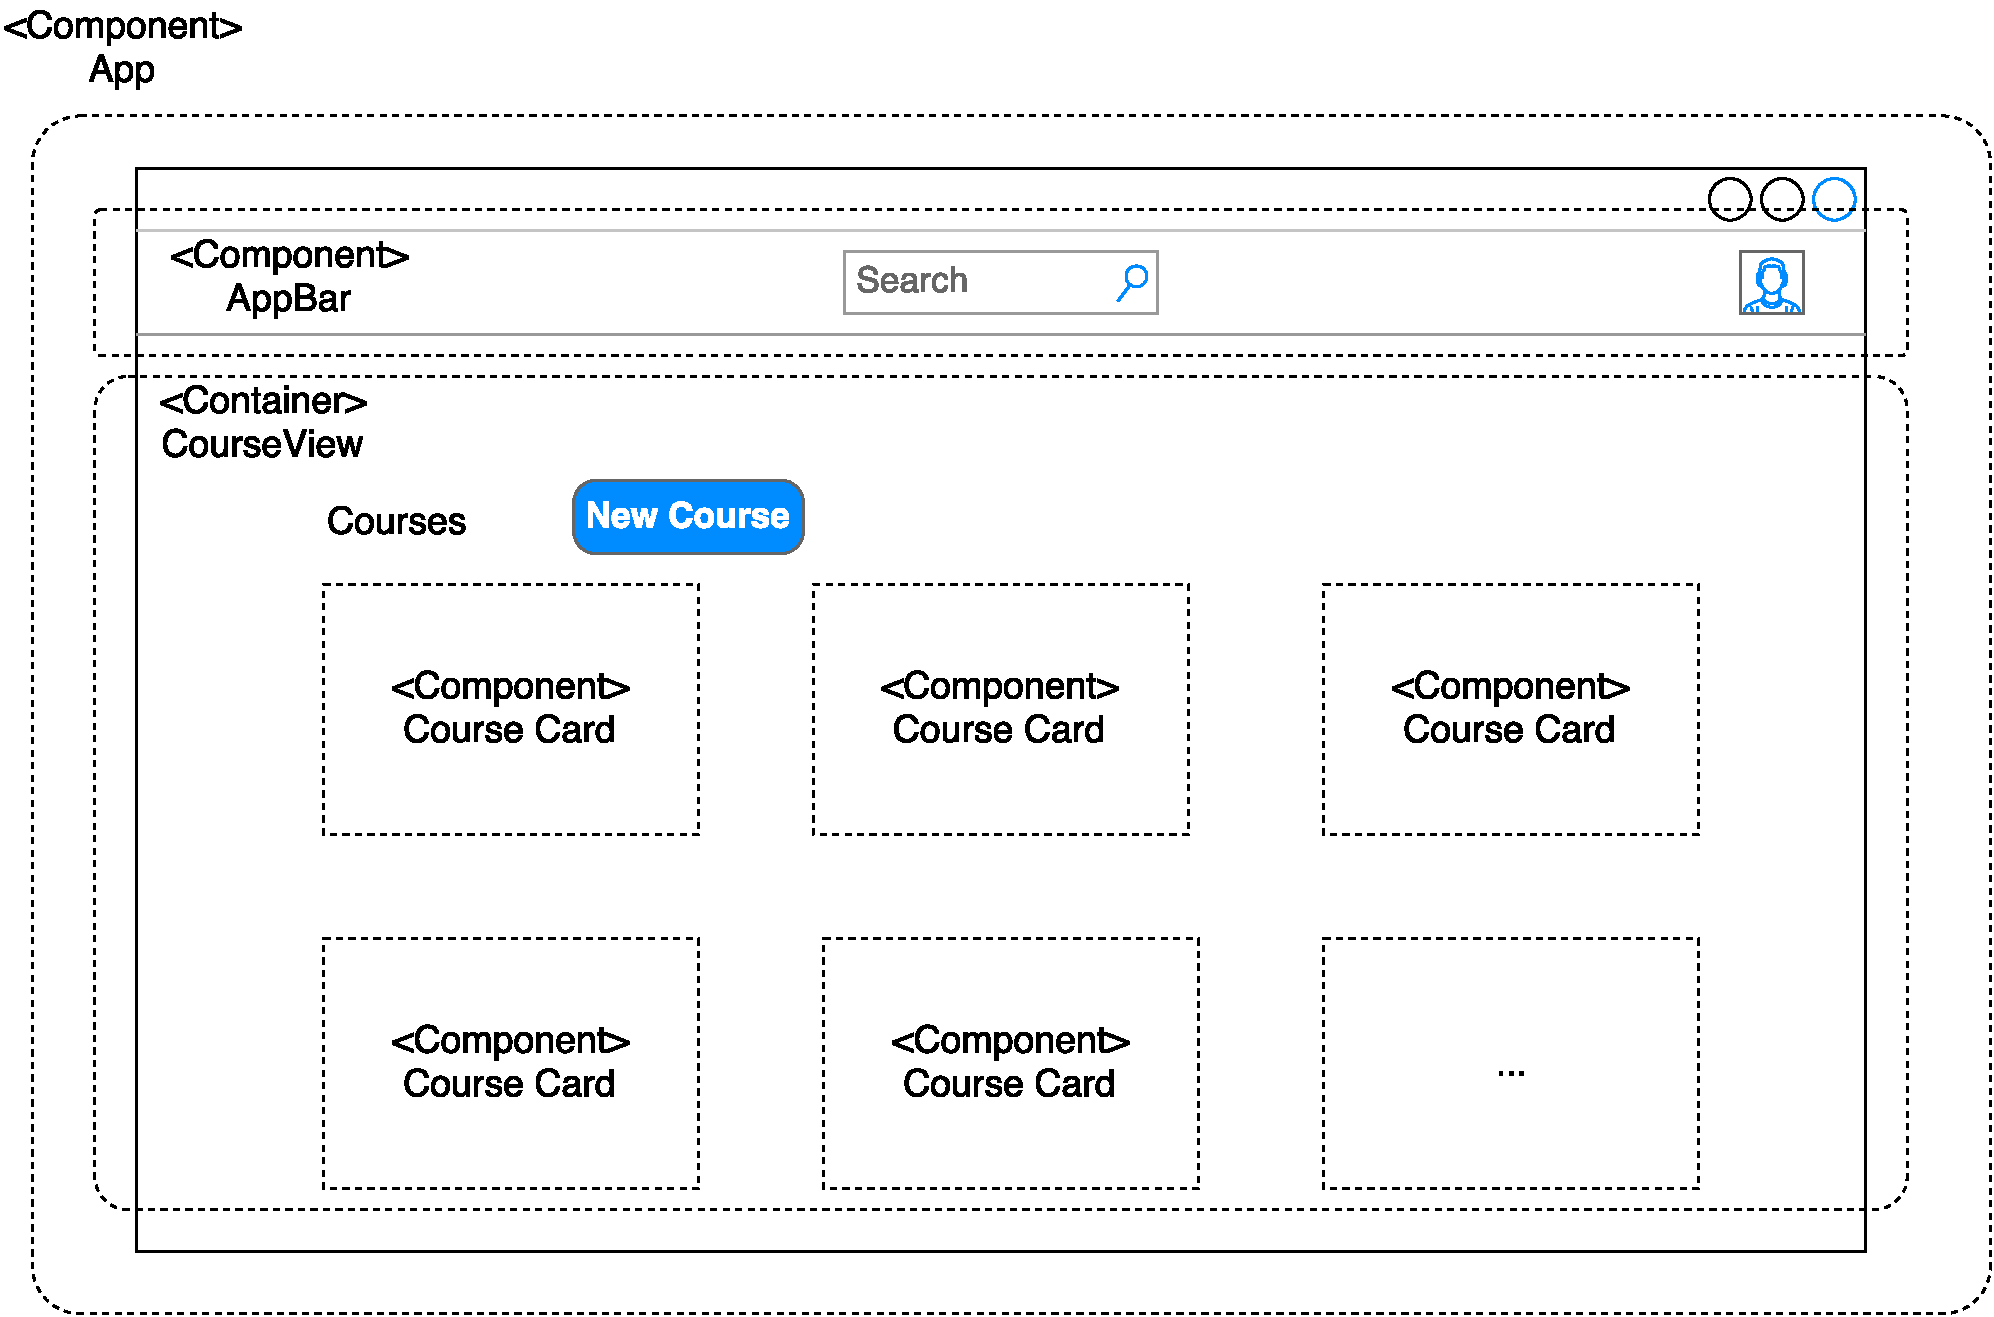
\includegraphics[width=1\textwidth]{Figures/imp-course-view-composition.pdf}
  \caption{Composition of components in courses' page}
  \label{fig:course-view-composition-imp}
\end{figure}
% Course Page. Composition, App bar, tab view, course page, course card ...

At the top of the view is a component called \textit{AppBar}, which is also composed with another component \textit{SearchBox}. \textit{ContentSection} is a container for the main content, which will be replaced and re-rendered if the context of router changes. In this example, the route \textit{/courses} is applied, and the component \textit{CourseView} is rendered into \textit{ContentSection}. 

\textit{CourseView} is also a composition of components: a list of \textit{CourseCard} components and also other components such as submit button component and popover component for creating new course. 

In principle, building other views is the same approach. Composition of components constructs the all views. With fine-grained components, the client app becomes much extensible and maintainable.


\subsection{Data Flow}\label{subsection:data-flow-react-imp}

Since data is passed as properties of components from top to bottom in the React application, maintaining data models between components and the data flow through components is a problem. \textit{Flux}\footnote{http://facebook.github.io/flux/} is a architecture which aims to solve this problem. Data flows in single direction, which keeps the process simple and ensures the correctness of view rendering.

There are four main concepts of Flux architecture: 
\begin{itemize}
  \item 
  \textbf{View}: view layer which references the data model and renders the data model into template.
  \item 
  \textbf{Action}: action made by view, trigger for processing data model, for example a mouse click event.
  \item 
  \textbf{Dispatcher}: receives the actions and run callback functions to modify the data model.
  \item 
  \textbf{Store}: stores the states of data, if the states of data are changed, store will notify the views to re-render with the new state of data.
\end{itemize}

\begin{figure}[!htbp]
  \centering
    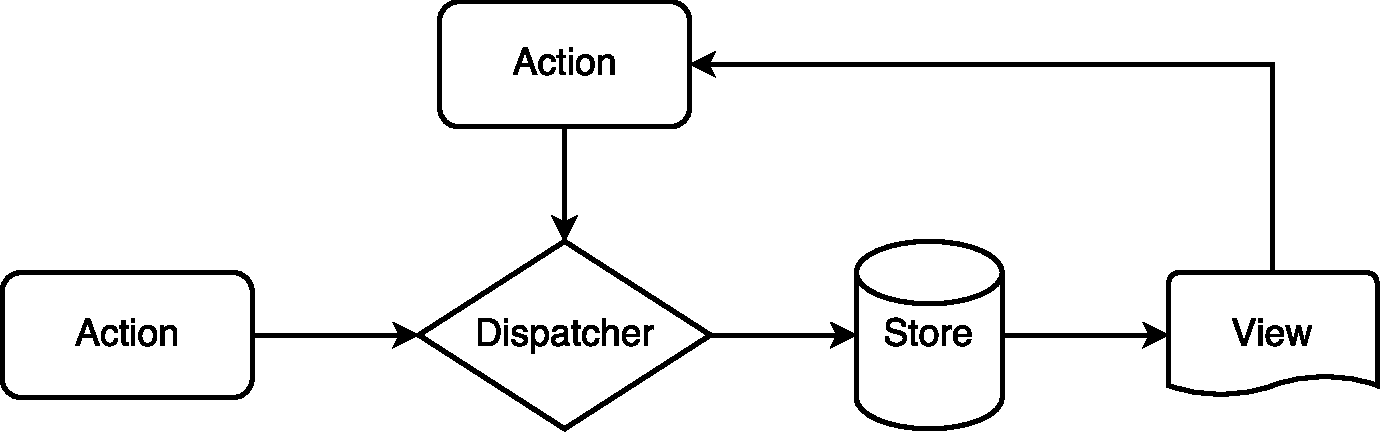
\includegraphics[width=0.9\textwidth]{Figures/imp-flux-arch.pdf}
  \caption{Data flow in Flux architecture}
  \label{fig:flux-arch-imp}
\end{figure}

The main process of data flow in Flux architecture is illustrated in figure \ref{fig:flux-arch-imp}. The key of Flux is unidirectional data flow. For example, user wants to submit a new answer to a certain question in Graphicuss system, as soon as the new answer is synchronized with server side, the new answer will be rendered into the answer list attached to the question. The process of data flow in this case is described as following:
\begin{enumerate}
  \item 
  User submits a new answer, \textit{Action(NEW\_ANSWER)} is triggered.
  \item 
  \textit{Action} requests the API for submitting new answer.
  \item 
  \textit{Dispatcher} receives the \textit{Action(NEW\_ANSWER)} and inserts an entry of this new answer into the \textit{answers} state which is stored in \textit{Store}.
  \item 
  Since the state of \textit{answers} is changed, \textit{Store} starts notifying the views to re-render.
  \item 
  Views re-render the templates with the new state of \textit{answers} which contains the new submission of answer.
\end{enumerate}
% Architecture Building Tool, Compile Workflow, Whiteboard, Socket, React?

\section{Drawing Tool for Graphicuss}
In this section, the implementation of converting Canvas to a storable data with JSON format is introduced. Afterwards, a drawing tool which provides user interfaces to draw various elements on Canvas is implemented.

\subsection{Objectified Canvas}

\subsubsection{Fabric.js}
Fabric.js\footnote{http://fabricjs.com/ - accessed 18 July 2016} is a powerful and simple Javascript HTML5 canvas library, which provides interactive object models on top of canvas elements. Since native Canvas only provides low-level APIs for creating elements, but not maintains the life cycle of elements on itself. Fabric.js solves this problem with objectifying native elements and encapsulating native methods for drawing elements. 

Instead of dealing with low-level APIs natively provided by Canvas, Fabric.js provides objectified model for elements with different shapes  on top of native methods. It takes charge of canvas state and rendering, make it possible to manipulate objects directly.


\subsubsection{Serialized Canvas}
Since all elements on the Canvas drawn by Fabric.js can be maintained as an object with properties like position, size and styles.
So the Canvas within Fabric.js can be simply serialized to a JSON object or other formats. 

Fabric.js provides a helper function called \textit{toJSON()}, which will serialize the canvas with canvas properties as well as all object models on the canvas. Code list \ref{list:serialized-canvas-imp} is an example that shows how the serialized output looks like if a rectangle object is created by using Fabric.js.

\begin{lstlisting}[language=JavaScript, caption=Serialized Canvas by Fabric.js , label={list:serialized-canvas-imp}]
var canvas = new fabric.Canvas();
canvas.backgroundColor = 'red';
canvas.add(new fabric.Rect({
  left: 50,
  top: 50,
  height: 20,
  width: 20,
  fill: 'green'
}));
console.log(JSON.stringify(canvas));
/* --- Output of serialized Canvas --- 
{"objects":[{"type":"rect","left":50,"top":50,"width":20,"height":20,"fill":"green","overlayFill":null,"stroke":null,"strokeWidth":1,"strokeDashArray":null,"scaleX":1,"scaleY":1,"angle":0,"flipX":false,"flipY":false,"opacity":1,"selectable":true,"hasControls":true,"hasBorders":true,"hasRotatingPoint":false,"transparentCorners":true,"perPixelTargetFind":false,"rx":0,"ry":0}],"background":"rgba(0, 0, 0, 0)"}
*/
\end{lstlisting}

Comparing with output generated by native Canvas mentioned in section \ref{sec:graphical-data-serialization-concept}, this serialized JSON object is not only efficient for storing, but also has the possibility for restoring all object models and re-rendering them on Canvas.

\subsection{Drawing Tool}
The drawing tool is developed on top of the library Fabric.js. It provides the functionalities such as drawing, styling, dragging and resizing of various elements. Not only graphical elements, texts could also be rendered and styled on the Canvas while using drawing tool.

Figure \ref{fig:drawing-tool-arch-imp} illustrates an overview of the drawing tool's architecture. 

\begin{figure}[!htbp]
  \centering
    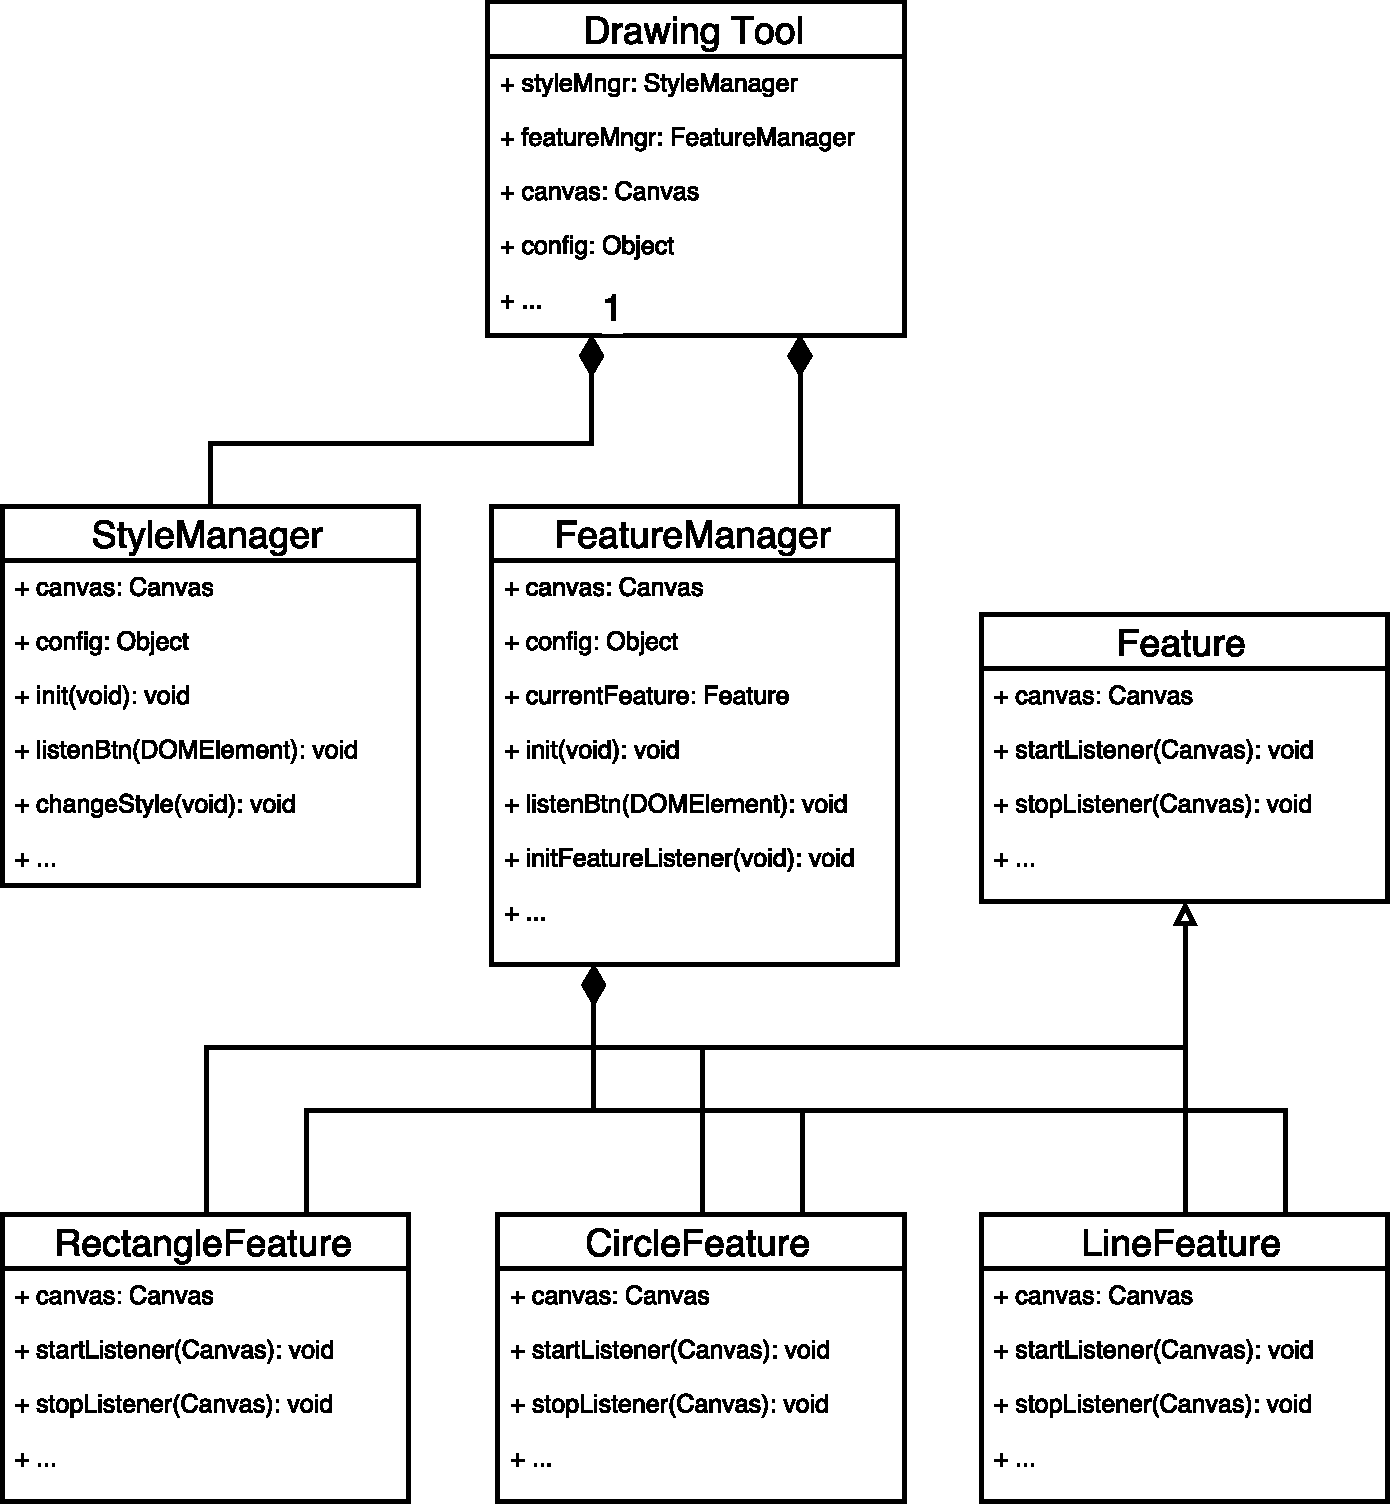
\includegraphics[width=1\textwidth]{Figures/imp-drawing-tool-arch.pdf}
  \caption{Architecture of drawing tool}
  \label{fig:drawing-tool-arch-imp}
\end{figure}

\subsubsection{Style Manager}
At the startup of drawing tool, \textit{StyleManager} is instantiated. \textit{StyleManager} receives the config instance, in which the DOM elements with relevant styling functionalities are defined. And in the \textit{init()} function of \textit{StyleManager}, listeners for the DOM elements are created. If the DOM elements are triggered by the user, \textit{StyleManager} will apply the chosen style to the active objects on the Canvas.

Code list \ref{list:style-manager-imp} takes the listener for DOM element of color picker, which is used for changing the color of an object on Canvas. It acquires the reference of color picker DOM from the config instance, and starts listening for the \textit{onchange} event. If the \textit{onchange} event is fired, the listener will set the object's \textit{fill} property to the color value. Afterwards, the canvas is re-rendered and the active object with new color is shown up.

\begin{lstlisting}[language=JavaScript, caption=Main process of StyleManager, label={list:style-manager-imp}]
class StyleManager {
  constructor(canvas, config){
    this._canvas = canvas;
    this._config = config;
  }
  init(){
    el = this._config['color-picker-dom']
    this._listenColor(el)
    // ... more styling listeners
  }
  _listenColor(el){
    let self = this;
    el.onchange = function(){
      var obj = self.canvas.getActiveObject();
      self._setObjStyle(obj, 'fill', el.value);
      canvas.renderAll();
    }
  }
  // ...
}
\end{lstlisting}


\subsubsection{Feature Manager \& Extensible Features}

In addition, a \textit{FeatureManager} is also created for managing different drawing functionalities. The basic idea of \textit{FeatureManager} is quite similar as \textit{StyleManager} mentioned above. It also listens for the DOM elements to toggle different drawing behaviours.

After that a specific drawing mode is triggered by user, \textit{FeatureManager} will assign listeners for specific mouse events on the Canvas and track the drawing behaviours. According to the mouse events triggered by user on the Canvas, the correlate objects will be rendered into the Canvas context.

\begin{lstlisting}[language=JavaScript, caption=Main process of FeatureManager, label={list:feature-manager-imp}]
class FeatureManager {
  constructor(canvas, config){
    this._canvas = canvas;
    this._config = config;
  }
  init(){
    el = this._config['text-feature-dom']
    this._listenText(el)
    // ... more features' listeners
  }
  _listenText(el){
    let textFeature = new TextFeature(this._canvas);
    el.onclick = (e) => { 
      this._clickHandler(text)
    }
  }
  // ...
}
class TextFeature{
  constructor(canvas){
    this._canvas = canvas;
  }
  startListen(){
    // tracking mouse event
  }
  stopListen(){
    // remove listeners
  }
}
\end{lstlisting}

Features, namely drawing modes are highly extensible on the drawing tool. \textit{TextFeature} in code list \ref{list:feature-manager-imp} is an example. All feature classes need to implement two interfaces \textit{startListen()} and \textit{stopListen()} basically. In \textit{startListen()}, listeners for tracking mouse events are defined. And in \textit{stopListen()}, all listeners should be removed. Both functions will be called by \textit{FeatureManager} when this drawing mode is toggled.

% \section{Difficulties and open Questions}
% % increment history!


\section{Conclusion}
Conclusion!



\chapter{Evaluation}
After the development approach has been motivated, designed and implemented in the previous chapters, an evaluation for both usability and data model  will take place in this part.


\section{Usability}
% 10 Usability Heuristics for User Interface Design, SUS(System Usability Scale)
Usability testing refers to evaluating a product or service by testing it with representative users. In principle, during a usability test, participants  will evaluate the system with quantitive metrics. 

The goal of usability testing is to collect the quantitive data, analyse the result and issue the usability problems with tested system. 

\subsection{System Usability Scale}

The System Usability Scale (SUS) offers a "quick and dirty", but relative reliable approach for measuring the usability\cite{brooke1996sus}.  It contains a 10 item questionnaire with five rating options for participants; from \textit{strongly agree} to \textit{strongly disagree}.


In order to calculate the SUS score, score contributions from each item should be calculated once separately at first. Score contribution will range from 0 to 4. For items with odd number, the score contribution should minus 1. For item with even number, the contribution is 5 minus the score. The sum of all scores is multiplied by 2.5 to obtain the overall value of SUS, which has a range of 0 to 100.

\begin{equation}
\label{formular:SUS}
SUS_{sum} = 2.5 \times \left (  \sum_{ i=1}^{5} \left ( a_{2i-1} - 1 \right ) + \sum_{ i=1}^{5} \left ( 5 - a_{2i} \right ) \right ) 
\end{equation}


\begin{table}[!htbp]
\centering
\begin{tabularx}{\textwidth}{@{}lXXXXXl@{}}
\toprule
Item(No.)   & A  & B  & C  & D  & E          & Average Score        \\ \midrule
1               & 3  & 4  & 3  & 4  & 4          & 3.6                     \\
2               & 2  & 1  & 1  & 1  & 2          & 1.4                     \\
3               & 5  & 4  & 4  & 5  & 4          & 4.4                     \\
4               & 1  & 2  & 1  & 2  & 2          & 1.6                     \\
5               & 4  & 4  & 3  & 4  & 5          & 4                     \\
6               & 4  & 5  & 4  & 3  & 4          & 4                     \\
7               & 5  & 4  & 4  & 5  & 5          & 4.6                     \\
8               & 3  & 3  & 2  & 1  & 3          & 2.4                     \\
9               & 5  & 4  & 3  & 4  & 5          & 4.2                     \\
10              & 2  & 3  & 2  & 1  & 2          & 2                     \\ \bottomrule        
\end{tabularx}
\caption{Score of SUS table}
\label{table:score-sus}
\end{table}

For the SUS testing of Graphicuss system, 5 participants are involved in the interview with SUS questionnaire, which is listed in appendix \ref{appendix:sus}. Each participant gives his own score contribution for each item, and the average score of each item is calculated. Table \ref{table:score-sus} shows the result.

According to the formula \ref{formular:SUS}, the final sum SUS score of the system is \textbf{73.5}. An article represents the mapping of adjective ratings to SUS score\cite{bangor2009determining}. And a \textbf{73.5} SUS score achieves the rating in a range of \textit{Good} to \textit{Excellent} when it is expressed by adjective ratings. 

The result reveals that the Graphicuss system achieves a relative high score in the general usability test. In general, users are able to learn to use this system very quickly. Without significant help, they can operate the system smoothly and unproblematically. 

% \cite{bangor2009determining} \cite{gackenheimer2015core}\cite{barron1998minimum}\cite{grunwald2005advances}\cite{ferraiolo2000scalable}\cite{fette2011websocket}\cite{geary2012core}\cite{richardson2008restful}\cite{pautasso2008restful}\cite{pimentel2012communicating}



\subsection{Interview based Usability Test}

Interviews with college students have been conducted in order to evaluate the system's usability as well as the fulfilment of requirements. 

Nielsen had a research about the relationship between the amount of test users and the percentage of problems they found. Figure \ref{fig:eval-nielsen} shows the result\cite{nielsen2001conduct}. Only 5 participants are already enough for discovering 75\% of usability problems in most cases. Therefore, for the interview of evaluation, 5 participants are invited. The key parameters of the interview are listed as follows. 

\begin{figure}[!htbp]
  \centering
    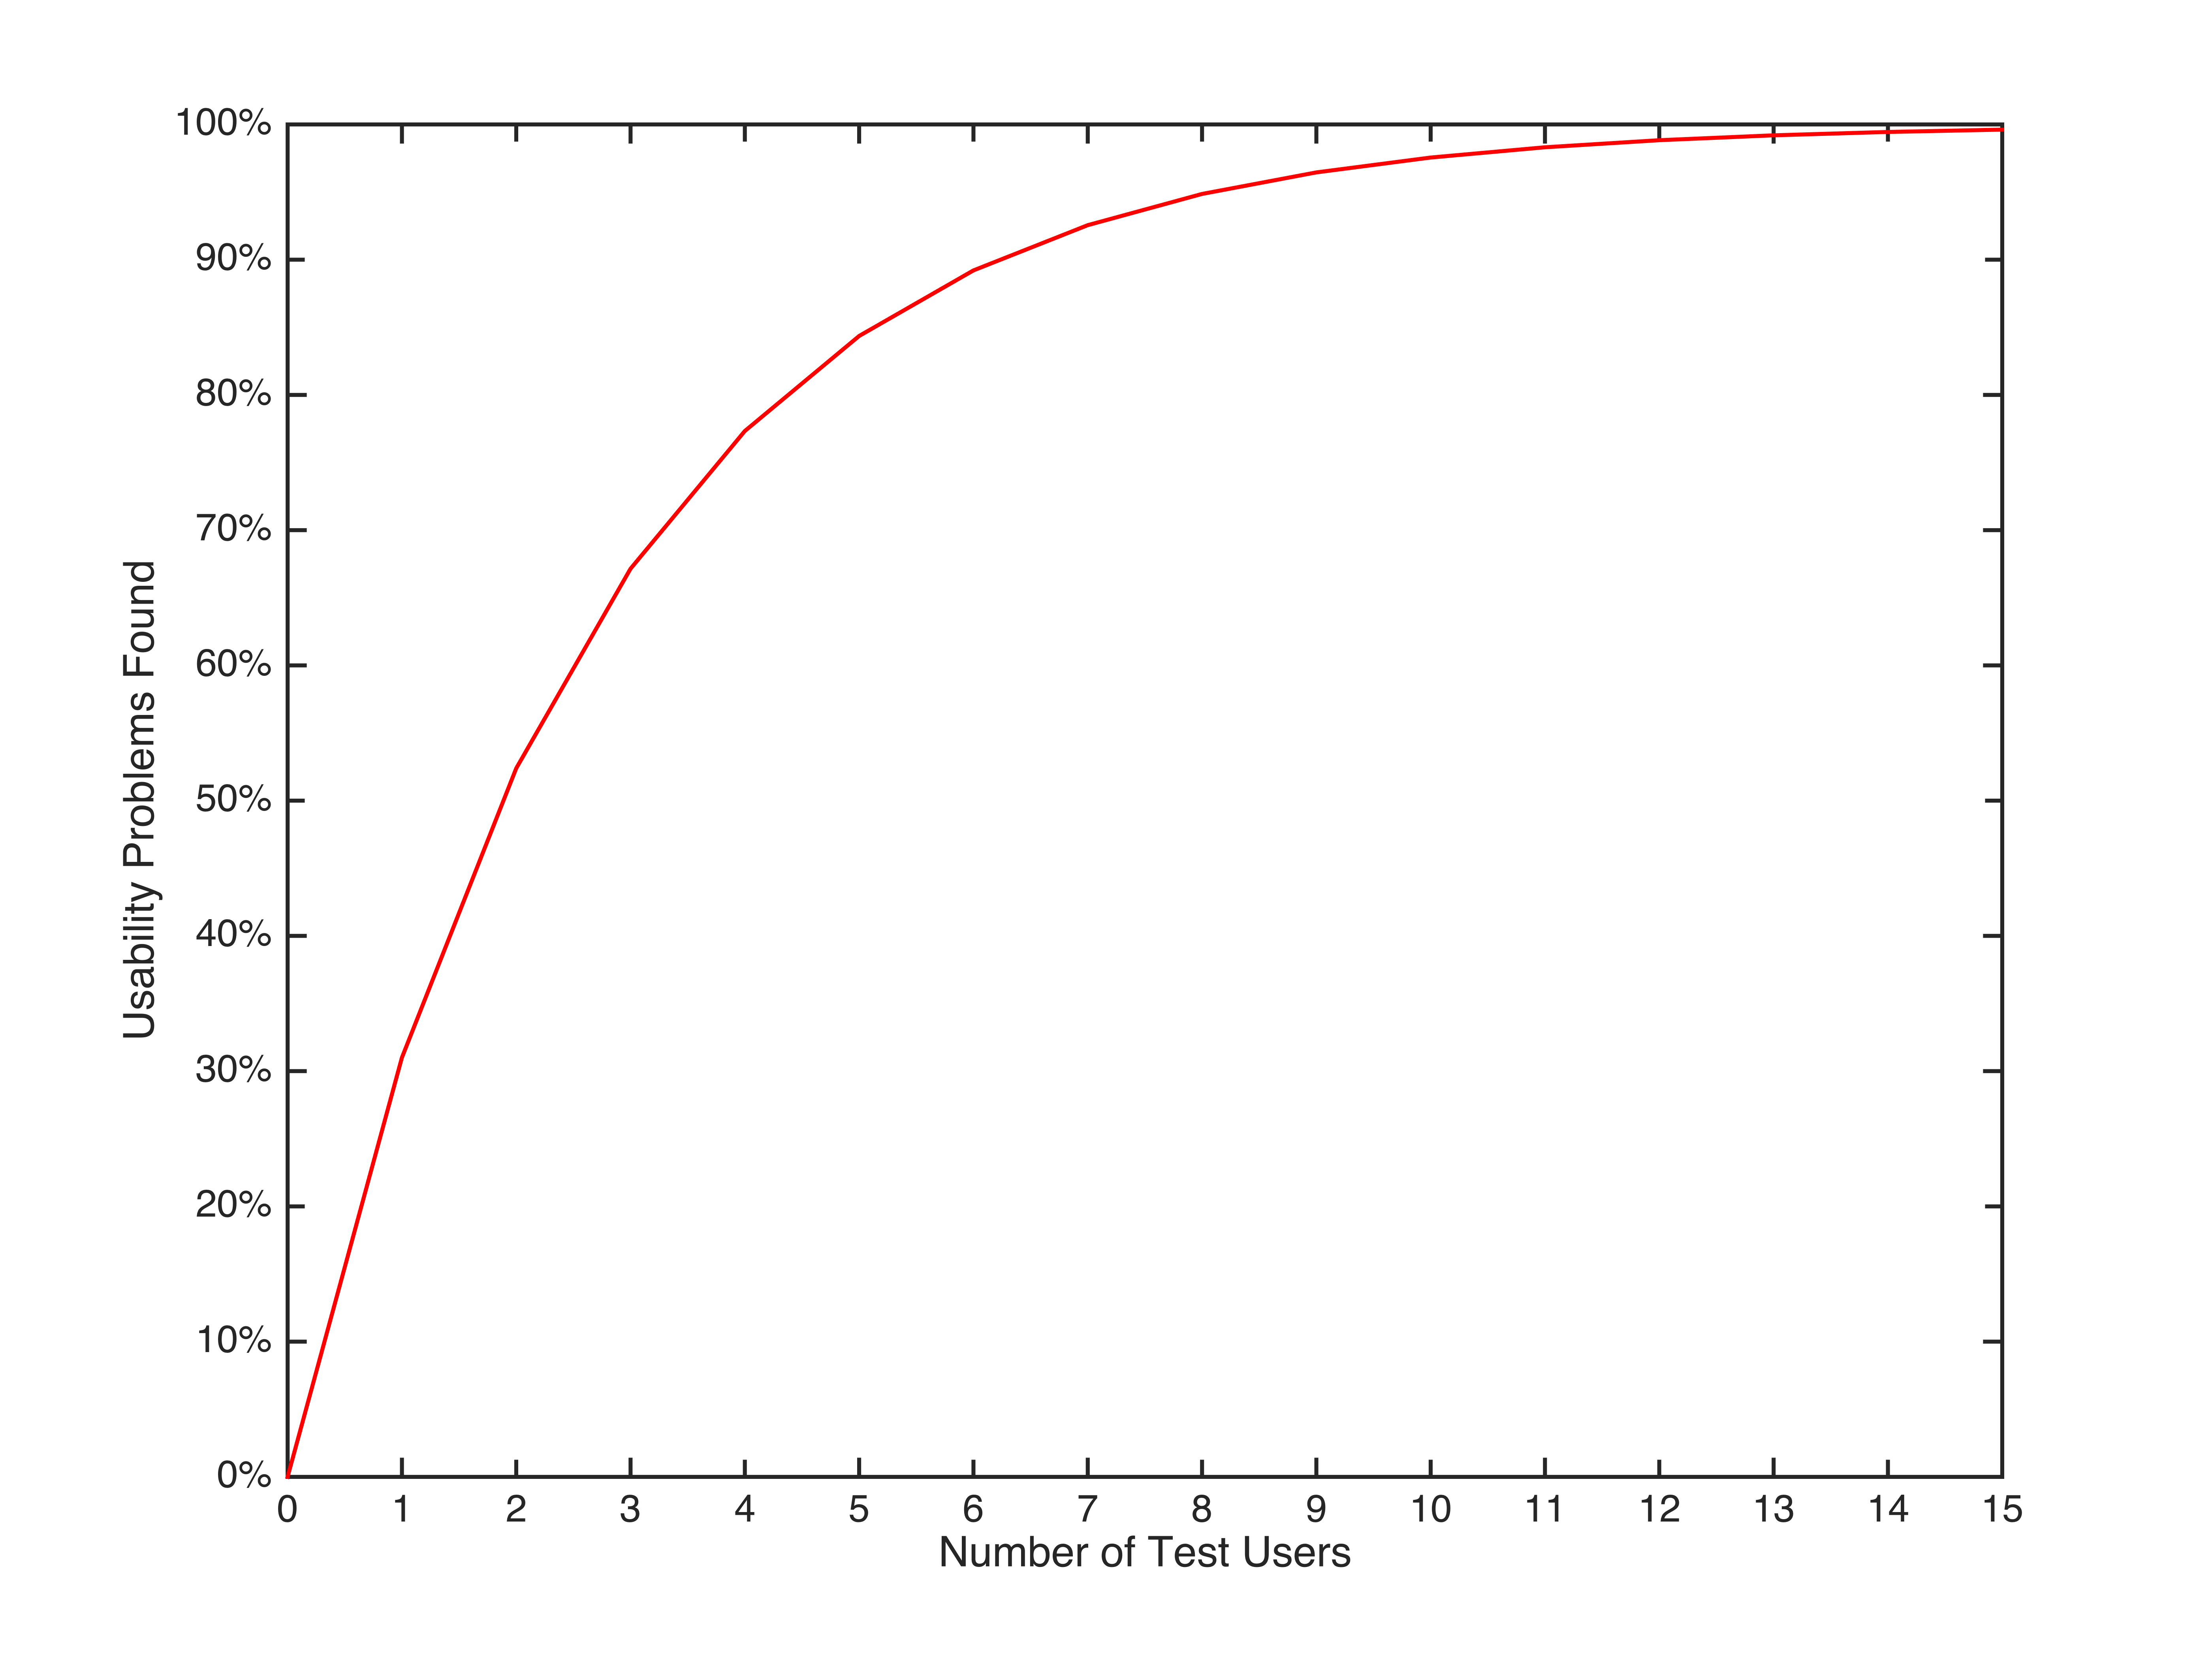
\includegraphics[width=0.8\textwidth]{Figures/eval-nielsen.png}
  \caption{Proportion of usability problems in an interface found by heuristic evaluation using various numbers of evaluators}
  \label{fig:eval-nielsen}
\end{figure}

\begin{itemize}
  \item  Interview type: Discussion and questions to be answered using a 5-point Likert scale with additional space for comments and feedback.
  \item  Number of questions: 10
  \item  Duration of each interview: 20-30 minutes
  \item  Time period of the conduction: 27th June 2016. The question sheet is attached to this thesis in Appendix \ref{appendix:interview}.
  \item  Interview conduction: 
  \begin{enumerate}
    \item Several courses are created at the very beginning before the interview is performed. 
    \item After the interview is started, interviewees are requested to sign up with their own accounts and search the certain course by the course code.
    \item Afterwards, they start questioning or answering within the certain course at the same time.
    \item Interviewees are also demanded to use the major functionalities of the system, especially the drawing tool and quote functionality.
    \item At last, the remaining 8 questions have been answered by the interviewees, followed by a final discussion of the results.
  \end{enumerate}
\end{itemize}

The overall results of the interviews are presented in table \ref{table:score-interview}, which contains the score rated by each interviewee and the average score of each question. 

\begin{table}[!htbp]
\centering
\begin{tabularx}{\textwidth}{@{}lXXXXXl@{}}
\toprule
Item(No.)       & A  & B  & C  & D  & E          & Average Score        \\ \midrule
1               & 5  & 4  & 4  & 5  & 5          & 4.6                     \\
2               & 4  & 5  & 5  & 4  & 4          & 4.4                     \\
3               & 5  & 4  & 4  & 5  & 4          & 4.4                     \\
4               & 4  & 3  & 4  & 3  & 4          & 3.6                    \\
5               & 4  & 3  & 3  & 3  & 2          & 3                     \\
6               & 4  & 5  & 4  & 5  & 4          & 4.4                     \\
7               & 5  & 5  & 5  & 5  & 4          & 4.8                     \\
8               & 2  & 3  & 3  & 2  & 2          & 2.4                     \\
9               & 3  & 4  & 5  & 4  & 3          & 3.8                     \\
10               & 2  & 3  & 1  & 2  & 1          & 1.8                     \\ \bottomrule    
\end{tabularx}
\caption{Score of each questions of the interview}
\label{table:score-interview}
\end{table}

\subsubsection{Analysis of General Functionalities}
Question 1-3 are designed for evaluating the main workflow of the system. Relative high score are made by interviewws while testing the main functionalities of the system such like searching for a certain course, submitting questions and answers.

One tester has raised the issue that the auto-generated code (e.g. \textit{dogP\_Iz8}) for querying the certain course is a little bit complex. Instead of a complex string with both alphabets and symbols, a simplified code which only has numbers would be accepted. In addition, interviewee C noticed that a pagination of the questions' list is required if the amount of question is getting greater.

\subsubsection{Analysis of Drawing Tool }
Question 4 is proposed to investigate the usability of the integrated text input in the drawing tool. Most interviewees are generally satisfied with the basic functionality of inputting a text string using the drawing tool. Tester B figured that the more stylings on the text should be implemented.

Most interviewees thought that the preset of the default elements were far not enough, which could be concluded from the Question 5. More shapes, which could be selected and drawn instantly, are highly required to be added into the preset. Otherwise, with the current elements of drawing shapes with the drawing tool, the expected graphical content is not able to be expressed precisely.

The history functionality of the drawing tool is productive according to the score rated in question 6. Undo/Redo function really helps the interviewees to correct the mistakes they made while using the drawing tool. Question 7 with the highest score shows that the modification on top of quoted content is convenient and useful.

\subsubsection{Analysis of Real-Time Functionality}

The real-time functionality is also investigated during the interview. All interviewees pointed out that the auto-odering of answers is not seamless and unconspicuous, which could also cause distraction while viewing the answers. Therefore, the scores of question 8 and 10 are quite low.

However, the majority of interviewees has the opinion that the real-time feature will significantly improve the interactivity of the system despite of the distraction caused while auto-ordering is performed.



\section{Rendering Performance}
% 10 Usability Heuristics for User Interface Design, SUS(System Usability Scale)

%\subsection{Evaluation Approach}

While the graphical data model space means the efficiency and capability  of server side, the graphical rendering performance plays a key role for the client side. Loading time of the web application is obviously an important part of user experience. To evaluate the graphical rendering performance, the rendering time in \textit{millisecond} is measured as the amount of components increases.

\begin{itemize}
  \item \textbf{Test Environment}: A representative size \textit{800*600} is chosen and tested on \textit{Chrome version 52}. In additional, the \textit{Chrome Dev Tool} is used for inspecting the performance metrics. CPU, which also has an impact on the result, runs at \textit{2.3 GHz}.
  \item \textbf{Metrics}: \textit{Total Time}, which includes the scripting time, rendering time and painting time, and \textit{Scripting Time} therefrom are measured along with increasing amounts of components drawn on the objectified Canvas. 
\end{itemize}

The approach of measurement is performed as follows:

\begin{enumerate}
  \item A graphical data model in JSON format is generated, which composes a certain amount of random components: \textit{Rectangle}, \textit{Circle} and \textit{Line}.
  \item Objectified Canvas starts parsing the graphical data, instantiating the components and render them on the Canvas.
  \item \textit{Chrome Dev Tool} is utilized to inspect the rendering timeline of step 2. Total time from loading to rendering and scripting time as a part of total time are recorded.
\end{enumerate}
In general, four tests are performed for both types of Canvas in two different sizes. 

Figure \ref{fig:eval-perf} illustrates the results of the test. As a result, two outcomes are concluded as follows.

\begin{figure}[!htbp]
  \centering
    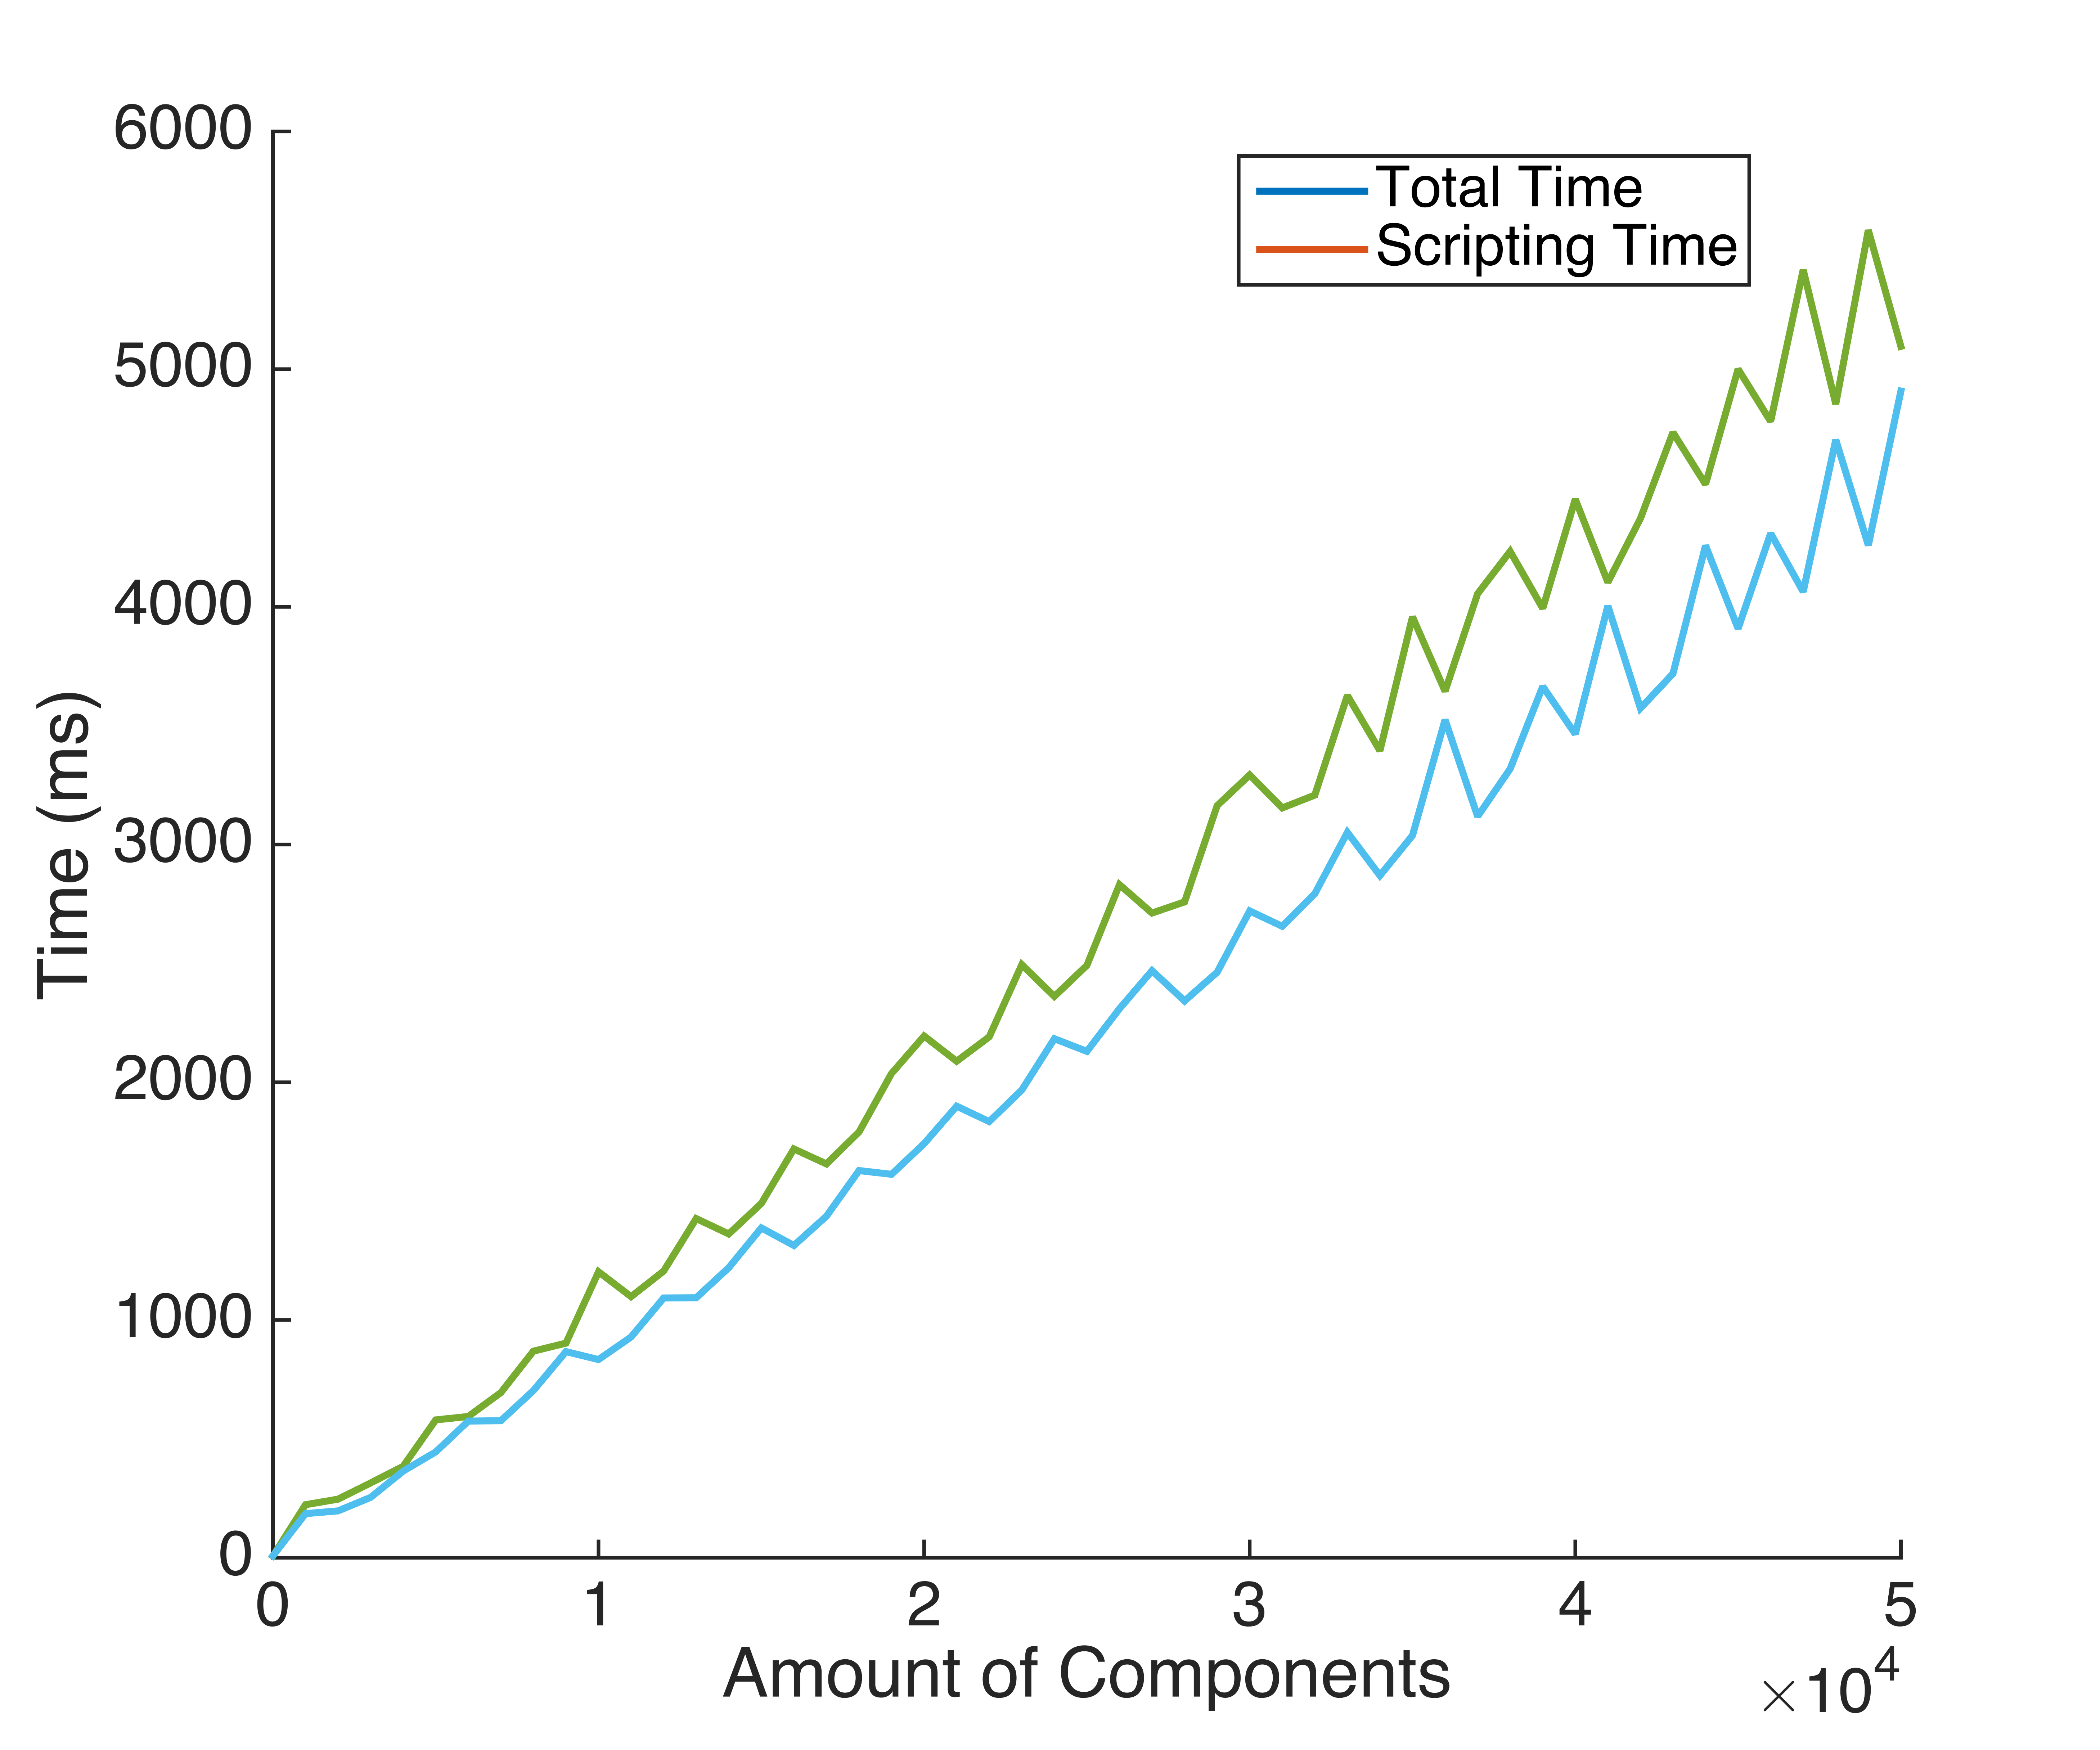
\includegraphics[width=1\textwidth]{Figures/eval-perf.png}
  \caption{Consumption of total time and scripting time in the rendering process of objectified Canvas}
  \label{fig:eval-perf}
\end{figure}

%\subsection{Analysis of Result }

\textbf{Rendering performance is approximately linear to the amount of components}. As shown in the figure \ref{fig:eval-perf}, the total time, which includes scripting time, rendering time and painting time is about 1000 ms when the amount of components is $1\times 10^{4}$. If the amount of Components reaches $5\times 10^{4}$, the total time increases to nearly 5000 ms.

\textbf{Scripting time has accounted for the majority of total time}. As a part of total time, the scripting time , which is also approximately linear, takes the most of time consumption while processing the rendering task. After the objectified Canvas has loaded the image data successfully, it will parse each component defined in the image data and instantiate them as well as add the objects into its own context. However, the actual rendering time, which is the difference of total time and scripting time, is only a fraction in the whole rendering process.

However, the performance test is performed with such a huge range of components' amount, which doesn't represent the usage in normal case. Considering the linearity of the rendering performance, drawing less than 1000 components, which are already huge enough for expressing the graphical content in the real world, will only spend less than 100 ms.

\section{Data Model Evaluation}
% 10 Usability Heuristics for User Interface Design, SUS(System Usability Scale)
In the section \ref{sec:graphical-data-serialization-concept} the raw output from native Canvas is briefly described, while the serialized graphical data model adopted in Graphicuss system is presented in section \ref{sec:drawing-imp}. A comparison of both data model within different dimensions is performed in this part.

\subsection{Evaluation Approach}



\subsection{Dimension: Size of Canvas}



\subsection{Dimension: Amounts of Components}


\begin{figure}[!htbp]
  \centering
    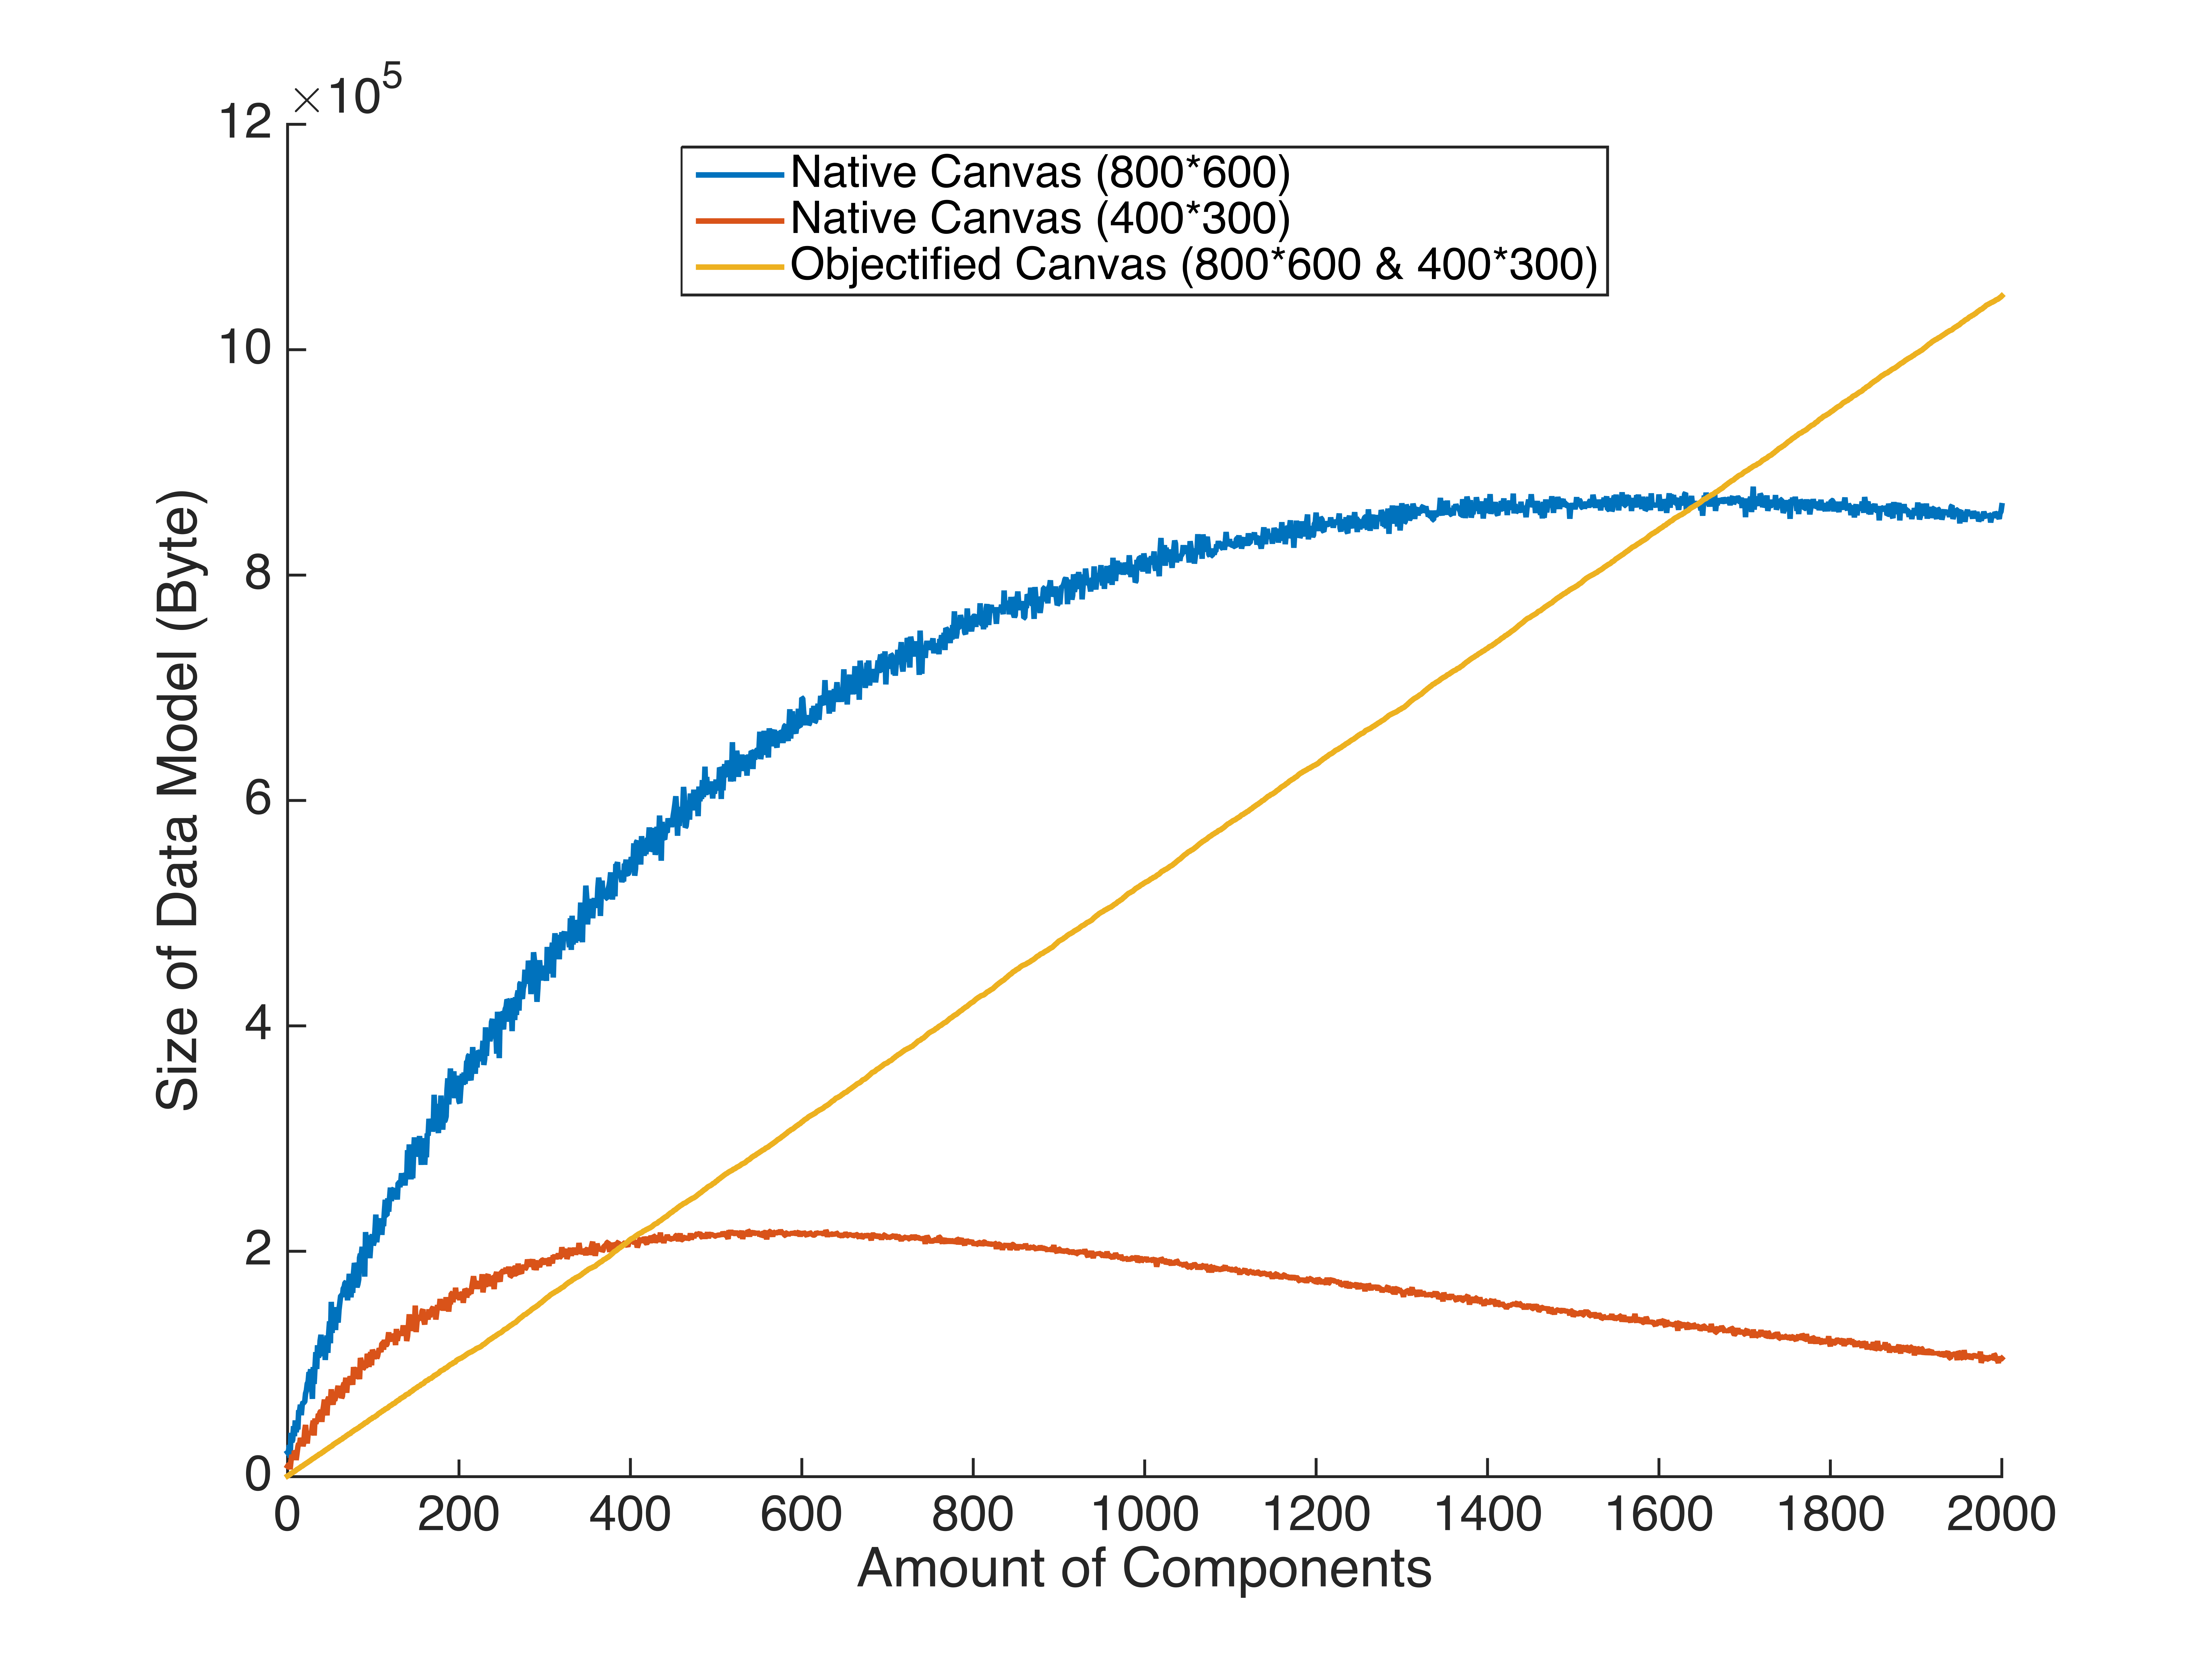
\includegraphics[width=1\textwidth]{Figures/eval-size.png}
  \caption{Comparison of data spaces of image data from native Canvas in two sizes(800*600, 400*300) and adopted graphical data model in Graphicuss}
  \label{fig:eval-nielsen}
\end{figure}



\section{Conclusion}
Conclusion!



\chapter{Conclusion and Future Work}
\section{Conclusion}

\subsection{Modern Web Application}

The discuss system is the cornerstone, which provides users the basic functionalities for discussion such like authentication, questioning and answering. The Single-Page-Application architecture is applied while concepting and implementing this discussion system. Since the client application and the server application are fully separated, the data definitions and data communication between two sides have also been discussed and implemented. RESTFul APIs within the system, which is used as a lightweight and universal web service for the data transmission, are designed and implemented on the server side.

Implementation details of building the client application using \textit{React.js} are also described. The concept of \textit{Componentization} is introduced, namely, all the views are actually compositions of various components. Fine-grained components are defined with templates and data representation logic inside.

In addition, in order to accelerate the development process, as well as the deployment process for further usage, an automated building workflow is also considered. 


\subsection{Objectified Canvas}

The graphical discussion contribution made by users, which is efficient for persistence purpose and is able to be restored back to the Canvas for the quote functionality, is the main topic of this thesis. For exploring the possibility, deficiencies of native Canvas are revealed. 

As a feasible approach to realize the feature mentioned above, an objectified Canvas is designed and implemented. Instead of exporting image data describing each pixel from native Canvas, the objectified Canvas outputs the graphical content to a serialized data  of all objects with various properties on its Canvas. 

In the evaluation phase, the storing efficiency of graphical data exported from objectified Canvas has been proved. Comparing to the image data outputted from native Canvas, the size of data model exported from objectified Canvas is much smaller, if the amount of components doesn't reach the thresholds which is basically a relative huge number.

The relationship of rendering performance of the objectified Canvas and amount of components has also been analyzed in the evaluation. As a result, the rendering performance is approximately linear to the amount of components. Moreover, as a part of the total time in the rendering process, the scripting time occupies the majority of time consumption. 


\subsection{Real-time communication}



Real-time communication, which enables the bi-directional communication between client and server, is also a focal point of this work. Arbitrary resources are able to be subscribed and users will get notified and acquire the newest data passively as the content of subscribed resource changes.

To achieve this goal, \textit{WebSocket} is applied as the basic real-time communication protocol. To broadcast data precisely through WebSocket to the users who subscribe the certain resources, a list which maps user socket to  resource id is maintained by server, after a WebSocket connection has been successfully established. As the state of  resource is changed, users who have subscribed this resource are notified with the new state of resource by querying the mapping relation in the list.


\section{Future Work}

Although the developed prototype of graphical discussion system covers the requirements and realizes the basic functionalities, some future researches and improvements are still needed to be done.

\textbf{Notification system could be extended for the discussion system.} For now, users won't get notified if new answers are posted under their own questions. Therefore, a notification system is proposed. Users would also be able to subscribe a certain question or class he interested in for further notifications if new contributions are made under it.

\textbf{More pre-defined shapes of components should be extended for the drawing tool.} According to the result of evaluation in section \ref{sec:eval-usability}, most users hold the idea that the preset of shapes in the drawing tool are far not enough. Therefore, the drawing tool should have provided more pre-defined components natively, which will significantly ease the drawing process and helps the user to express the precise; graphical content as expected. 

\textbf{Divers stylings of text on the drawing tool should be implemented.} The developed drawing tool already provides the possibility to input textual content for now. However the current styling of the text is still circumscribed. At present, adjusting the size or color of the text is already possible. More stylings such as strikethrough, list format could be extended in the future. 

% At least to 72

\newpage
\addcontentsline{toc}{chapter}{List of Figures}
\listoffigures

\newpage
\addcontentsline{toc}{chapter}{List of Tables}
\listoftables

\newpage
\addcontentsline{toc}{chapter}{List of Codes}
\lstlistoflistings

% \newpage
% \addcontentsline{toc}{chapter}{Glossary}
% \printglossary



\begin{appendices}


\newcolumntype{P}{>{\centering\arraybackslash}p{0.75cm}}
\newcolumntype{L}{>{\raggedright\arraybackslash}m{0.2\textwidth}}
\newcolumntype{R}{>{\raggedleft\arraybackslash}m{0.2\textwidth}}

\newcommand{\printtblhdr}{%
  \hfill
  \begingroup
  \setlength\tabcolsep{0pt}%
  \begin{tabularx}{0.41\textwidth}{ @{} l *{3}X r @{} }
    \multicolumn{2}{l}{\bfseries\shortstack[l]{Strongly\\ Disagree}}
    &&
    \multicolumn{2}{l}{\bfseries\shortstack[r]{Strongly\\ Agree}}
    \\
  \end{tabularx}
  \endgroup
}

\newcommand{\usetbl}{%
  \begin{tabular}{@{}|*5{P|}@{}}
    \hline
    1 & 2 & 3 & 4 & 5 \\
    \hline
  \end{tabular}
}

\newcommand\prop[1]{%
  \item
  \parbox[t]{0.5\textwidth}{#1}%
  \qquad
  \parbox[t]{0.5\textwidth}{\usetbl}%
}






\chapter{System Usability Scale Table} \label{appendix:sus}

\printtblhdr

\begin{enumerate}
\prop{I think that I would like to use this system frequently}

\prop{I found the system unnecessarily complex}

\prop{I thought the system was easy to use}

\prop{I think that I would need the support of a technical person to be able to use this system}

\prop{I found the various functions in this system were well integrated}

\prop{I thought there was too much inconsistency in this system}

\prop{I would imagine that most people would learn to use this system very quickly}

\prop{I found the system very cumbersome to use}

\prop{I felt very confident using the system}

\prop{I needed to learn a lot of things before I could get going with this system}

\end{enumerate}

\let\cleardoublepage\clearpage


\chapter{System Usability Interview} \label{appendix:interview}


\printtblhdr

\begin{enumerate}
\prop{I could find the certain course created by tutor.}

\prop{The process of asking a question or answering a question was simple.}

\prop{Voting score would help to locate the useful contribution.}

\prop{Integrated text input in the drawing tool would helps express the textual content.}

\prop{The drawing tool provided enough elements ready to be drawn.}

\prop{Quoting and modifying on top of others\' contributions are useful.}

\prop{I found the history function(undo redo) of drawing tool was really necessary.}

\prop{Auto-ordering of answers was seamless and unconspicuous.}

\prop{I found the real-time feature was interactive.}

\prop{The real-time feature didn't cause distraction while viewing the answers.}

\end{enumerate}



\end{appendices}



\addcontentsline{toc}{chapter}{References}
\bibliographystyle{ieeetr}
\bibliography{references}

\end{document}
